% Options for packages loaded elsewhere
\PassOptionsToPackage{unicode}{hyperref}
\PassOptionsToPackage{hyphens}{url}
%
\documentclass[
]{article}
\usepackage{amsmath,amssymb}
\usepackage{iftex}
\ifPDFTeX
  \usepackage[T1]{fontenc}
  \usepackage[utf8]{inputenc}
  \usepackage{textcomp} % provide euro and other symbols
\else % if luatex or xetex
  \usepackage{unicode-math} % this also loads fontspec
  \defaultfontfeatures{Scale=MatchLowercase}
  \defaultfontfeatures[\rmfamily]{Ligatures=TeX,Scale=1}
\fi
\usepackage{lmodern}
\ifPDFTeX\else
  % xetex/luatex font selection
  \setmainfont[]{Arial}
\fi
% Use upquote if available, for straight quotes in verbatim environments
\IfFileExists{upquote.sty}{\usepackage{upquote}}{}
\IfFileExists{microtype.sty}{% use microtype if available
  \usepackage[]{microtype}
  \UseMicrotypeSet[protrusion]{basicmath} % disable protrusion for tt fonts
}{}
\makeatletter
\@ifundefined{KOMAClassName}{% if non-KOMA class
  \IfFileExists{parskip.sty}{%
    \usepackage{parskip}
  }{% else
    \setlength{\parindent}{0pt}
    \setlength{\parskip}{6pt plus 2pt minus 1pt}}
}{% if KOMA class
  \KOMAoptions{parskip=half}}
\makeatother
\usepackage{xcolor}
\usepackage[margin=1in]{geometry}
\usepackage{graphicx}
\makeatletter
\def\maxwidth{\ifdim\Gin@nat@width>\linewidth\linewidth\else\Gin@nat@width\fi}
\def\maxheight{\ifdim\Gin@nat@height>\textheight\textheight\else\Gin@nat@height\fi}
\makeatother
% Scale images if necessary, so that they will not overflow the page
% margins by default, and it is still possible to overwrite the defaults
% using explicit options in \includegraphics[width, height, ...]{}
\setkeys{Gin}{width=\maxwidth,height=\maxheight,keepaspectratio}
% Set default figure placement to htbp
\makeatletter
\def\fps@figure{htbp}
\makeatother
\setlength{\emergencystretch}{3em} % prevent overfull lines
\providecommand{\tightlist}{%
  \setlength{\itemsep}{0pt}\setlength{\parskip}{0pt}}
\setcounter{secnumdepth}{-\maxdimen} % remove section numbering
\usepackage{titling}
\pretitle{\begin{flushleft}}
\posttitle{\end{flushleft}}
\usepackage{pdflscape}
\newcommand{\blandscape}{\begin{landscape}}
\newcommand{\elandscape}{\end{landscape}}
\usepackage{float}
\usepackage{booktabs}
\usepackage{longtable}
\usepackage{array}
\usepackage{multirow}
\usepackage{wrapfig}
\usepackage{colortbl}
\usepackage{pdflscape}
\usepackage{tabu}
\usepackage{threeparttable}
\usepackage{threeparttablex}
\usepackage[normalem]{ulem}
\usepackage{makecell}
\usepackage{xcolor}
\ifLuaTeX
  \usepackage{selnolig}  % disable illegal ligatures
\fi
\usepackage{bookmark}
\IfFileExists{xurl.sty}{\usepackage{xurl}}{} % add URL line breaks if available
\urlstyle{same}
\hypersetup{
  hidelinks,
  pdfcreator={LaTeX via pandoc}}

\author{}
\date{\vspace{-2.5em}}

\begin{document}

\renewcommand{\arraystretch}{1.4}

\section{Key Demographic Patterns of Mexican Population in Chicago and
Cook County, and the Chicago MSA Over
Time}\label{key-demographic-patterns-of-mexican-population-in-chicago-and-cook-county-and-the-chicago-msa-over-time}

\begin{table}[H]
\centering
\begin{threeparttable}
\caption{\label{tab:unnamed-chunk-3}Mexican Population for 10 Cities with the Largest Share of Mexican Population, 2018-2022 (ACS 5-year Estimates)}
\centering
\fontsize{8}{10}\selectfont
\begin{tabular}[t]{>{\raggedright\arraybackslash}p{7em}>{\raggedleft\arraybackslash}p{5.5em}>{\raggedleft\arraybackslash}p{5.5em}>{\raggedleft\arraybackslash}p{5.5em}>{\raggedleft\arraybackslash}p{5.5em}>{\raggedleft\arraybackslash}p{5.5em}>{\raggedleft\arraybackslash}p{5.5em}}
\toprule
\multicolumn{1}{>{\centering\arraybackslash}p{7em}}{\begingroup\fontsize{7.5}{9.5}\selectfont \textbf{City Name}\endgroup} & \multicolumn{1}{>{\centering\arraybackslash}p{5.5em}}{\begingroup\fontsize{7.5}{9.5}\selectfont \textbf{Total Population}\endgroup} & \multicolumn{1}{>{\centering\arraybackslash}p{5.5em}}{\begingroup\fontsize{7.5}{9.5}\selectfont \textbf{Hispanic or Latino Population}\endgroup} & \multicolumn{1}{>{\centering\arraybackslash}p{5.5em}}{\begingroup\fontsize{7.5}{9.5}\selectfont \textbf{\% Hispanic or Latino of Total Population}\endgroup} & \multicolumn{1}{>{\centering\arraybackslash}p{5.5em}}{\begingroup\fontsize{7.5}{9.5}\selectfont \textbf{Total Mexican Population}\endgroup} & \multicolumn{1}{>{\centering\arraybackslash}p{5.5em}}{\begingroup\fontsize{7.5}{9.5}\selectfont \textbf{\% Mexicans of Total Population}\endgroup} & \multicolumn{1}{>{\centering\arraybackslash}p{5.5em}}{\begingroup\fontsize{7.5}{9.5}\selectfont \textbf{\% Mexicans of Hispanic or Latino Population}\endgroup}\\
\midrule
Los Angeles & 3,881,041 & 1,865,763 & 48.1\% & 1,196,186 & 30.8\% & 64.1\%\\
San Antonio & 1,445,662 & 951,823 & 65.8\% & 808,918 & 56.0\% & 85.0\%\\
Houston & 2,296,253 & 1,029,429 & 44.8\% & 686,373 & 29.9\% & 66.7\%\\
Phoenix & 1,609,456 & 691,205 & 43.0\% & 607,389 & 37.7\% & 87.9\%\\
Chicago & 2,710,105 & 787,050 & 29.0\% & 581,376 & 21.5\% & 73.9\%\\
El Paso & 677,181 & 552,434 & 81.6\% & 519,100 & 76.7\% & 94.0\%\\
Dallas & 1,300,642 & 551,447 & 42.4\% & 449,290 & 34.5\% & 81.5\%\\
San Diego & 1,383,987 & 416,630 & 30.1\% & 353,790 & 25.6\% & 84.9\%\\
New York City & 8,622,467 & 2,503,005 & 29.0\% & 338,119 & 3.9\% & 13.5\%\\
Fort Worth & 924,663 & 325,185 & 35.2\% & 271,493 & 29.4\% & 83.5\%\\
\bottomrule
\end{tabular}
\begin{tablenotes}
\small
\item [] \footnotesize{Data Sources:  IPUMS NHGIS, University of Minnesota, www.nhgis.org (2018-2022 American Community
Survey 5-year Estimates). Tabulations by Great Cities Institute. 2018-2022 American Community Survey 5-year Estimates, U.S. Census Bureau, https://data.census.gov/.}
\end{tablenotes}
\end{threeparttable}
\end{table}

\begin{table}[H]
\centering
\begin{threeparttable}
\caption{\label{tab:unnamed-chunk-4}Mexican Population, Income, and Mexican Homeownership Rate for 10 Metropolitan Areas with the Largest Share of Mexican Population, 2018-2022 (ACS 5-year Estimates)}
\centering
\fontsize{8}{10}\selectfont
\begin{tabular}[t]{>{\raggedright\arraybackslash}p{14.2em}>{\raggedleft\arraybackslash}p{5.1em}>{\raggedleft\arraybackslash}p{5.1em}>{\raggedleft\arraybackslash}p{5.1em}>{\raggedleft\arraybackslash}p{5.1em}>{\raggedleft\arraybackslash}p{5.1em}>{\raggedleft\arraybackslash}p{5.1em}}
\toprule
\multicolumn{1}{>{\centering\arraybackslash}p{14.2em}}{\begingroup\fontsize{7.5}{9.5}\selectfont \textbf{Metro Name}\endgroup} & \multicolumn{1}{>{\centering\arraybackslash}p{5.1em}}{\begingroup\fontsize{7.5}{9.5}\selectfont \textbf{Total Population}\endgroup} & \multicolumn{1}{>{\centering\arraybackslash}p{5.1em}}{\begingroup\fontsize{7.5}{9.5}\selectfont \textbf{Total Mexican Population}\endgroup} & \multicolumn{1}{>{\centering\arraybackslash}p{5.1em}}{\begingroup\fontsize{7.5}{9.5}\selectfont \textbf{\% Mexicans of Total Population}\endgroup} & \multicolumn{1}{>{\centering\arraybackslash}p{5.1em}}{\begingroup\fontsize{7.5}{9.5}\selectfont \textbf{Mean Income}\endgroup} & \multicolumn{1}{>{\centering\arraybackslash}p{5.1em}}{\begingroup\fontsize{7.5}{9.5}\selectfont \textbf{Median Income}\endgroup} & \multicolumn{1}{>{\centering\arraybackslash}p{5.1em}}{\begingroup\fontsize{7.5}{9.5}\selectfont \textbf{Mexican Home Ownership Rate}\endgroup}\\
\midrule
Los Angeles-Long Beach-Anaheim, CA Metro Area & 13,111,917 & 4,488,186 & 34.2\% & \$44,800 & \$34,447 & 43.2\%\\
Riverside-San Bernardino-Ontario, CA Metro Area & 4,610,050 & 2,086,735 & 45.3\% & \$45,104 & \$35,072 & 62.0\%\\
Houston-The Woodlands-Sugar Land, TX Metro Area & 7,142,603 & 1,925,395 & 27.0\% & \$46,129 & \$35,072 & 62.2\%\\
Dallas-Fort Worth-Arlington, TX Metro Area & 7,673,379 & 1,795,650 & 23.4\% & \$43,669 & \$35,000 & 62.2\%\\
Chicago-Naperville-Elgin, IL-IN-WI Metro Area & 9,566,955 & 1,696,231 & 17.7\% & \$44,024 & \$35,072 & 63.0\%\\
Phoenix-Mesa-Chandler, AZ Metro Area & 4,864,209 & 1,310,430 & 26.9\% & \$43,295 & \$35,824 & 59.1\%\\
San Antonio-New Braunfels, TX Metro Area & 2,570,862 & 1,220,362 & 47.5\% & \$44,964 & \$35,670 & 63.4\%\\
San Diego-Chula Vista-Carlsbad, CA Metro Area & 3,289,701 & 983,086 & 29.9\% & \$47,261 & \$35,072 & 43.2\%\\
McAllen-Edinburg-Mission, TX Metro Area & 873,167 & 771,024 & 88.3\% & \$39,783 & \$29,226 & 70.0\%\\
El Paso, TX Metro Area & 867,161 & 677,323 & 78.1\% & \$40,855 & \$30,500 & 67.1\%\\
\bottomrule
\end{tabular}
\begin{tablenotes}
\small
\item [] \footnotesize{Note: The data includes all employed individuals, regardless of whether they work full-time or part-time.}
\item [] \footnotesize{Data Source: IPUMS USA, University of Minnesota, www.ipums.org (2018-2022 American Community Survey 5-year Estimates). Tabulations by Great Cities Institute.}
\end{tablenotes}
\end{threeparttable}
\end{table}

\begin{table}[H]
\centering
\begin{threeparttable}
\caption{\label{tab:unnamed-chunk-5}Mexican Population, Income, and Mexican Homeownership Rate for 10 Counties with the Largest Share of Mexican Population, 2018-2022 (ACS 5-year Estimates)}
\centering
\fontsize{8}{10}\selectfont
\begin{tabular}[t]{>{\raggedright\arraybackslash}p{14.2em}>{\raggedleft\arraybackslash}p{5.1em}>{\raggedleft\arraybackslash}p{5.1em}>{\raggedleft\arraybackslash}p{5.1em}>{\raggedleft\arraybackslash}p{5.1em}>{\raggedleft\arraybackslash}p{5.1em}>{\raggedleft\arraybackslash}p{5.1em}}
\toprule
\multicolumn{1}{>{\centering\arraybackslash}p{14.2em}}{\begingroup\fontsize{7.5}{9.5}\selectfont \textbf{County Name}\endgroup} & \multicolumn{1}{>{\centering\arraybackslash}p{5.1em}}{\begingroup\fontsize{7.5}{9.5}\selectfont \textbf{Total Population}\endgroup} & \multicolumn{1}{>{\centering\arraybackslash}p{5.1em}}{\begingroup\fontsize{7.5}{9.5}\selectfont \textbf{Total Mexican Population}\endgroup} & \multicolumn{1}{>{\centering\arraybackslash}p{5.1em}}{\begingroup\fontsize{7.5}{9.5}\selectfont \textbf{\% Mexicans of Total Population}\endgroup} & \multicolumn{1}{>{\centering\arraybackslash}p{5.1em}}{\begingroup\fontsize{7.5}{9.5}\selectfont \textbf{Mean Income}\endgroup} & \multicolumn{1}{>{\centering\arraybackslash}p{5.1em}}{\begingroup\fontsize{7.5}{9.5}\selectfont \textbf{Median Income}\endgroup} & \multicolumn{1}{>{\centering\arraybackslash}p{5.1em}}{\begingroup\fontsize{7.5}{9.5}\selectfont \textbf{Mexican Home Ownership Rate}\endgroup}\\
\midrule
Los Angeles County, California & 9,936,690 & 3,586,953 & 36.1\% & \$44,286 & \$34,447 & 44.2\%\\
Harris County, Texas & 4,726,177 & 1,452,364 & 30.7\% & \$44,571 & \$34,589 & 58.9\%\\
Maricopa County, Arizona & 4,430,871 & 1,191,488 & 26.9\% & \$43,204 & \$35,400 & 57.8\%\\
Riverside County, California & 2,429,487 & 1,074,125 & 44.2\% & \$45,047 & \$35,072 & 64.8\%\\
Bexar County, Texas & 2,014,059 & 1,039,250 & 51.6\% & \$44,801 & \$35,595 & 62.2\%\\
Cook County, Illinois & 5,225,367 & 1,034,038 & 19.8\% & \$44,090 & \$35,072 & 60.2\%\\
San Bernardino County, California & 2,180,563 & 1,012,610 & 46.4\% & \$45,164 & \$35,072 & 59.1\%\\
San Diego County, California & 3,289,701 & 983,086 & 29.9\% & \$47,261 & \$35,072 & 43.2\%\\
Orange County, California & 3,175,227 & 901,233 & 28.4\% & \$46,716 & \$35,072 & 39.1\%\\
Dallas County, Texas & 2,604,053 & 858,197 & 33.0\% & \$40,705 & \$33,994 & 59.0\%\\
\bottomrule
\end{tabular}
\begin{tablenotes}
\small
\item [] \footnotesize{Note: The data includes all employed individuals, regardless of whether they work full-time or part-time.}
\item [] \footnotesize{Data Source: IPUMS USA, University of Minnesota, www.ipums.org (2018-2022 American Community Survey 5-year Estimates). Tabulations by Great Cities Institute.}
\end{tablenotes}
\end{threeparttable}
\end{table}

\begingroup\fontsize{8}{10}\selectfont

\begin{ThreePartTable}
\begin{TableNotes}
\item \footnotesize{Data Source: IPUMS NHGIS, University of Minnesota, www.nhgis.org (2018-2022 American Community Survey 5-year Estimates). Tabulations by Great Cities Institute.}
\end{TableNotes}
\begin{longtable}[t]{>{\raggedright\arraybackslash}p{14.2em}>{\raggedleft\arraybackslash}p{6.12em}>{\raggedleft\arraybackslash}p{6.12em}>{\raggedleft\arraybackslash}p{6.12em}>{\raggedleft\arraybackslash}p{6.12em}>{\raggedleft\arraybackslash}p{6.12em}}
\caption{\label{tab:unnamed-chunk-6}Mexican and Hispanic or Latino Population in Chicago, Cook County, and Collar Counties, 2018-2022 (ACS 5-year Estimates)}\\
\toprule
\multicolumn{1}{>{\centering\arraybackslash}p{14.2em}}{\begingroup\fontsize{8}{10}\selectfont \textbf{Area}\endgroup} & \multicolumn{1}{>{\centering\arraybackslash}p{6.12em}}{\begingroup\fontsize{8}{10}\selectfont \textbf{Mexican Population}\endgroup} & \multicolumn{1}{>{\centering\arraybackslash}p{6.12em}}{\begingroup\fontsize{8}{10}\selectfont \textbf{Hispanic or Latino Population}\endgroup} & \multicolumn{1}{>{\centering\arraybackslash}p{6.12em}}{\begingroup\fontsize{8}{10}\selectfont \textbf{Total Population}\endgroup} & \multicolumn{1}{>{\centering\arraybackslash}p{6.12em}}{\begingroup\fontsize{8}{10}\selectfont \textbf{\% Mexican of Hispanic or Latino}\endgroup} & \multicolumn{1}{>{\centering\arraybackslash}p{6.12em}}{\begingroup\fontsize{8}{10}\selectfont \textbf{\% Mexican of Total Population}\endgroup}\\
\midrule
Chicago & 581,376 & 787,050 & 2,710,105 & 73.9\% & 21.5\%\\
Cook County Outside of Chicago & 452,662 & 565,432 & 2,515,262 & 80.1\% & 18.0\%\\
Collar County & 514,133 & 643,183 & 3,168,879 & 79.9\% & 16.2\%\\
\bottomrule
\insertTableNotes
\end{longtable}
\end{ThreePartTable}
\endgroup{}

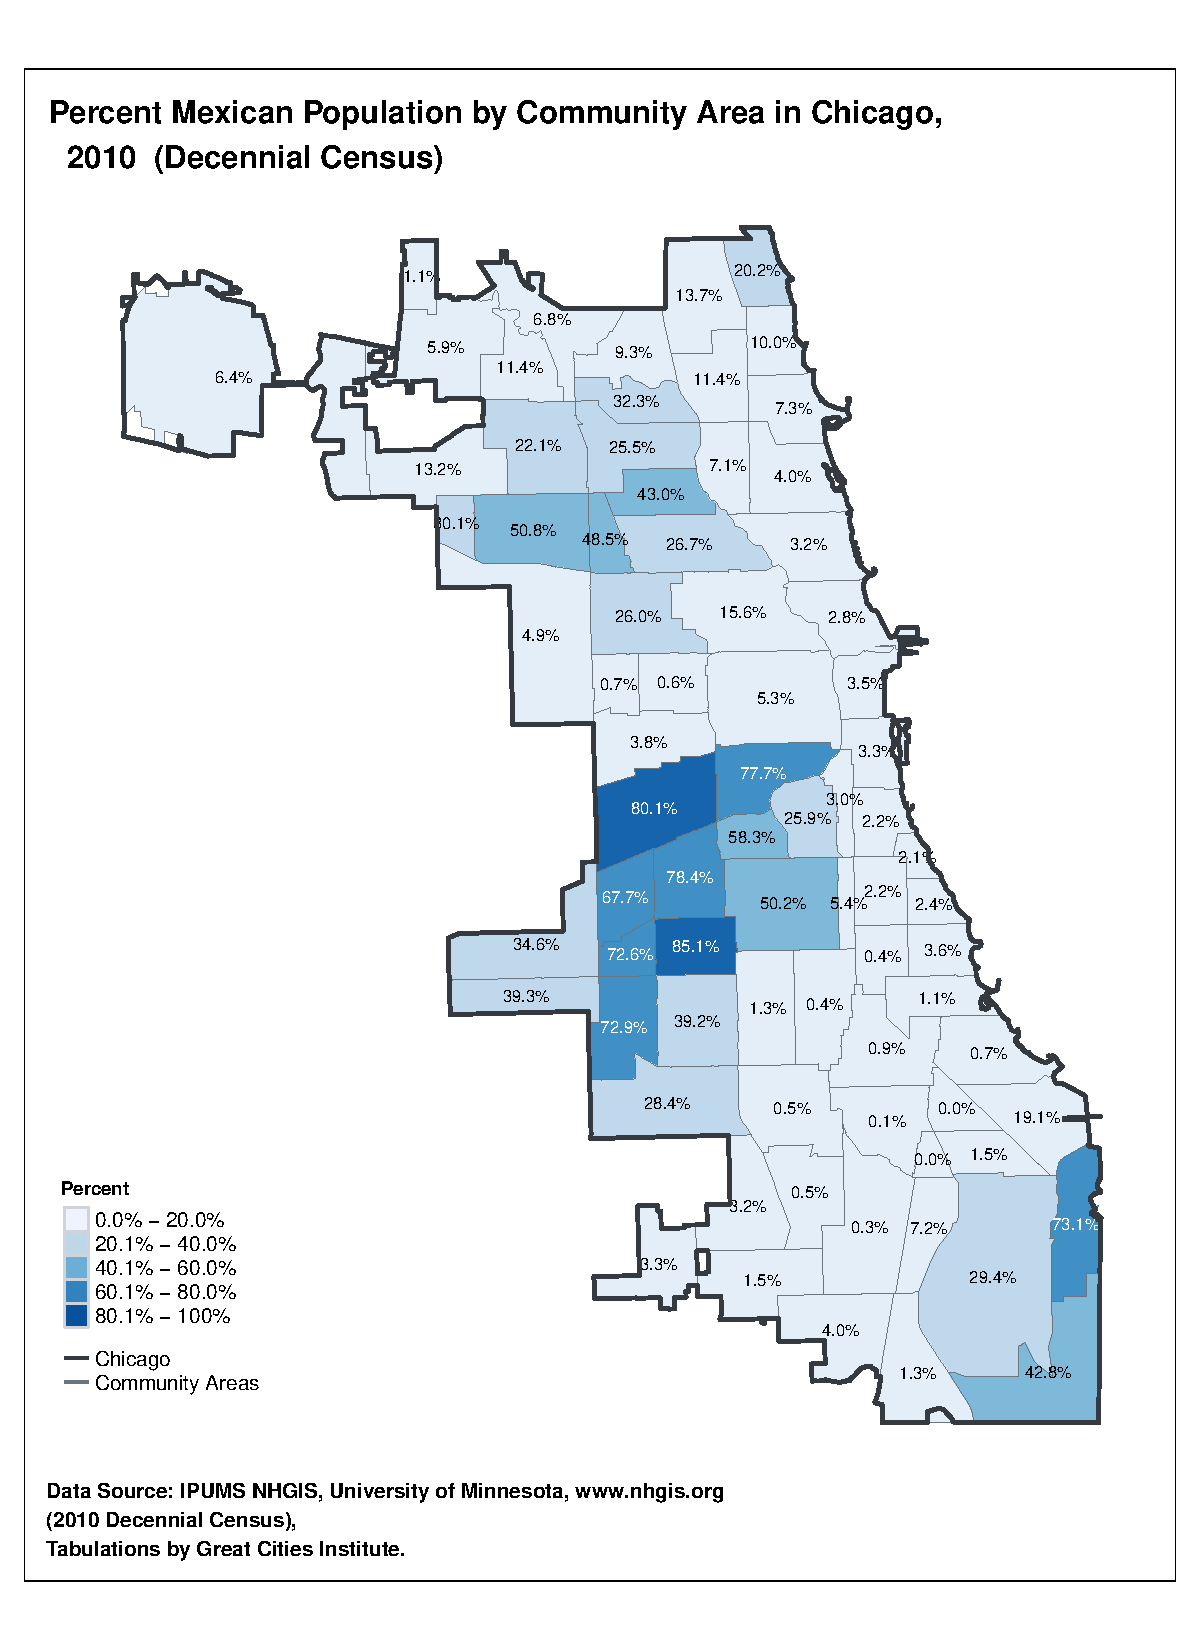
\includegraphics{combined_collar_county_10_files/figure-latex/unnamed-chunk-7-1.pdf}

\begin{landscape}

\begingroup\fontsize{8}{10}\selectfont

\begin{ThreePartTable}
\begin{TableNotes}
\item \footnotesize{Data Source: IPUMS NHGIS, University of Minnesota, www.nhgis.org (1990, 2000, 2010 Decennial Censuses, and 2018-2022 American Community Survey 5-year Estimates). Tabulations by Great Cities Institute. }
\end{TableNotes}
\begin{longtable}[t]{>{\raggedright\arraybackslash}p{14.2em}>{\raggedleft\arraybackslash}p{4.8em}>{\raggedleft\arraybackslash}p{4.8em}>{\raggedleft\arraybackslash}p{4.8em}>{\raggedleft\arraybackslash}p{4.8em}>{\raggedleft\arraybackslash}p{4.8em}>{\raggedleft\arraybackslash}p{4.8em}>{\raggedleft\arraybackslash}p{4.8em}>{\raggedleft\arraybackslash}p{4.8em}>{\raggedleft\arraybackslash}p{4.8em}>{\raggedleft\arraybackslash}p{4.8em}}
\caption{\label{tab:unnamed-chunk-8}Mexican Population in Chicago, Cook County, and Collar Counties, 1990, 2000, 2010 (Decennial Censuses), and 2018-2022 (ACS 5-year Estimates)}\\
\toprule
\multicolumn{1}{c}{\bgroup\fontsize{8}{10}\selectfont \textbf{Area}\egroup{}} & \multicolumn{2}{c}{\bgroup\fontsize{8}{10}\selectfont \textbf{1990}\egroup{}} & \multicolumn{2}{c}{\bgroup\fontsize{8}{10}\selectfont \textbf{2000}\egroup{}} & \multicolumn{2}{c}{\bgroup\fontsize{8}{10}\selectfont \textbf{2010}\egroup{}} & \multicolumn{2}{c}{\bgroup\fontsize{8}{10}\selectfont \textbf{2018-2022}\egroup{}} & \multicolumn{2}{c}{\bgroup\fontsize{8}{10}\selectfont \textbf{\makecell[c]{Change from\\1990 to 2018-2022}}\egroup{}} \\
\cmidrule(l{3pt}r{3pt}){1-1} \cmidrule(l{3pt}r{3pt}){2-3} \cmidrule(l{3pt}r{3pt}){4-5} \cmidrule(l{3pt}r{3pt}){6-7} \cmidrule(l{3pt}r{3pt}){8-9} \cmidrule(l{3pt}r{3pt}){10-11}
\multicolumn{1}{>{\centering\arraybackslash}p{14.2em}}{\begingroup\fontsize{8}{10}\selectfont \textbf{}\endgroup} & \multicolumn{1}{>{\centering\arraybackslash}p{4.8em}}{\begingroup\fontsize{8}{10}\selectfont \textbf{Number}\endgroup} & \multicolumn{1}{>{\centering\arraybackslash}p{4.8em}}{\begingroup\fontsize{8}{10}\selectfont \textbf{Percent}\endgroup} & \multicolumn{1}{>{\centering\arraybackslash}p{4.8em}}{\begingroup\fontsize{8}{10}\selectfont \textbf{Number}\endgroup} & \multicolumn{1}{>{\centering\arraybackslash}p{4.8em}}{\begingroup\fontsize{8}{10}\selectfont \textbf{Percent}\endgroup} & \multicolumn{1}{>{\centering\arraybackslash}p{4.8em}}{\begingroup\fontsize{8}{10}\selectfont \textbf{Number}\endgroup} & \multicolumn{1}{>{\centering\arraybackslash}p{4.8em}}{\begingroup\fontsize{8}{10}\selectfont \textbf{Percent}\endgroup} & \multicolumn{1}{>{\centering\arraybackslash}p{4.8em}}{\begingroup\fontsize{8}{10}\selectfont \textbf{Number}\endgroup} & \multicolumn{1}{>{\centering\arraybackslash}p{4.8em}}{\begingroup\fontsize{8}{10}\selectfont \textbf{Percent}\endgroup} & \multicolumn{1}{>{\centering\arraybackslash}p{4.8em}}{\begingroup\fontsize{8}{10}\selectfont \textbf{Number}\endgroup} & \multicolumn{1}{>{\centering\arraybackslash}p{4.8em}}{\begingroup\fontsize{8}{10}\selectfont \textbf{Percent Change}\endgroup}\\
\midrule
Chicago & 352,543 & 12.7\% & 530,452 & 18.3\% & 577,894 & 21.5\% & 581,376 & 21.5\% & 228,833 & 64.9\%\\
Cook County Outside of Chicago & 113,222 & 4.9\% & 255,971 & 10.3\% & 384,069 & 15.3\% & 452,662 & 18.0\% & 339,440 & 299.8\%\\
Kane County & 35,583 & 11.2\% & 80,870 & 20.0\% & 139,009 & 27.0\% & 140,614 & 27.2\% & 105,031 & 295.2\%\\
Lake County & 27,226 & 5.3\% & 71,153 & 11.0\% & 111,952 & 15.9\% & 127,212 & 17.8\% & 99,986 & 367.2\%\\
DuPage County & 24,703 & 3.2\% & 63,135 & 7.0\% & 96,039 & 10.5\% & 103,194 & 11.1\% & 78,491 & 317.7\%\\
\addlinespace
Will County & 16,582 & 4.6\% & 35,416 & 7.1\% & 90,355 & 13.3\% & 108,834 & 15.6\% & 92,252 & 556.3\%\\
McHenry County & 4,988 & 2.7\% & 15,881 & 6.1\% & 28,796 & 9.3\% & 34,279 & 11.0\% & 29,291 & 587.2\%\\
\bottomrule
\insertTableNotes
\end{longtable}
\end{ThreePartTable}
\endgroup{}

\end{landscape}

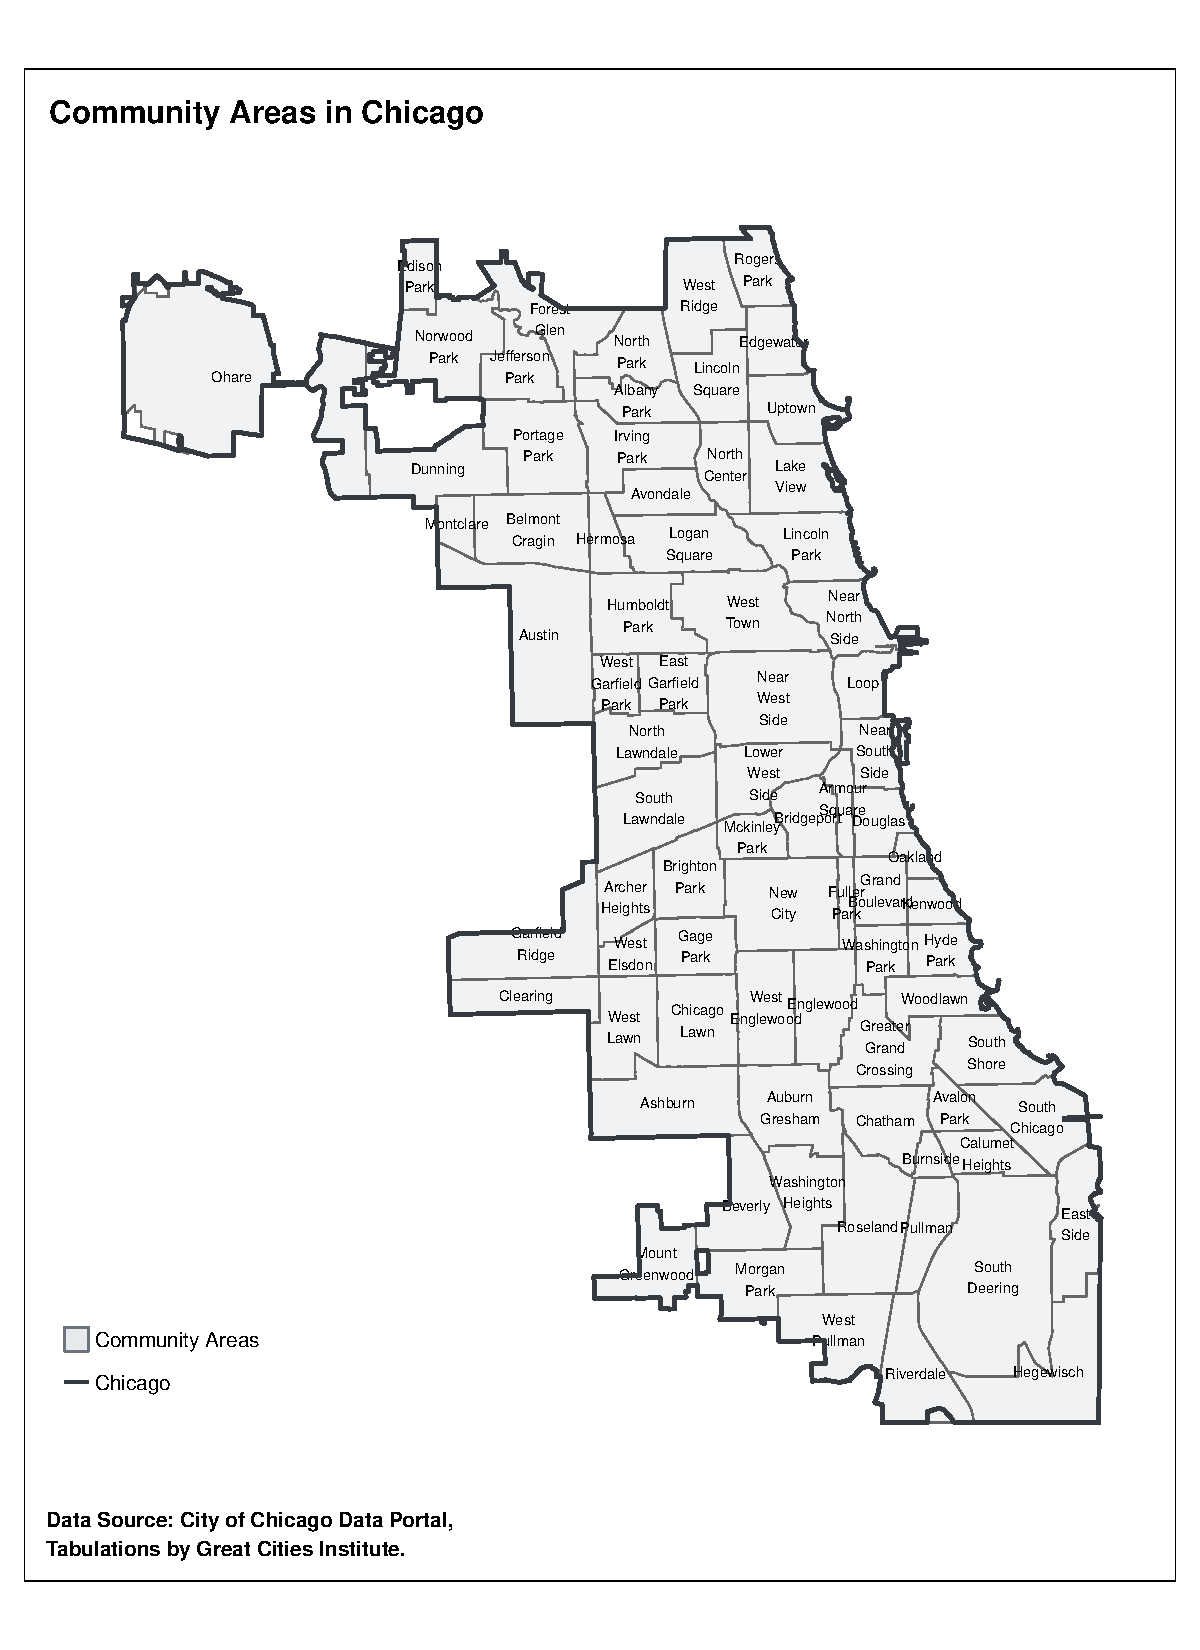
\includegraphics{combined_collar_county_10_files/figure-latex/unnamed-chunk-9-1.pdf}

\includegraphics{combined_collar_county_10_files/figure-latex/unnamed-chunk-11-1.pdf}

\includegraphics{combined_collar_county_10_files/figure-latex/unnamed-chunk-12-1.pdf}

\includegraphics{combined_collar_county_10_files/figure-latex/unnamed-chunk-13-1.pdf}

\includegraphics{combined_collar_county_10_files/figure-latex/unnamed-chunk-14-1.pdf}

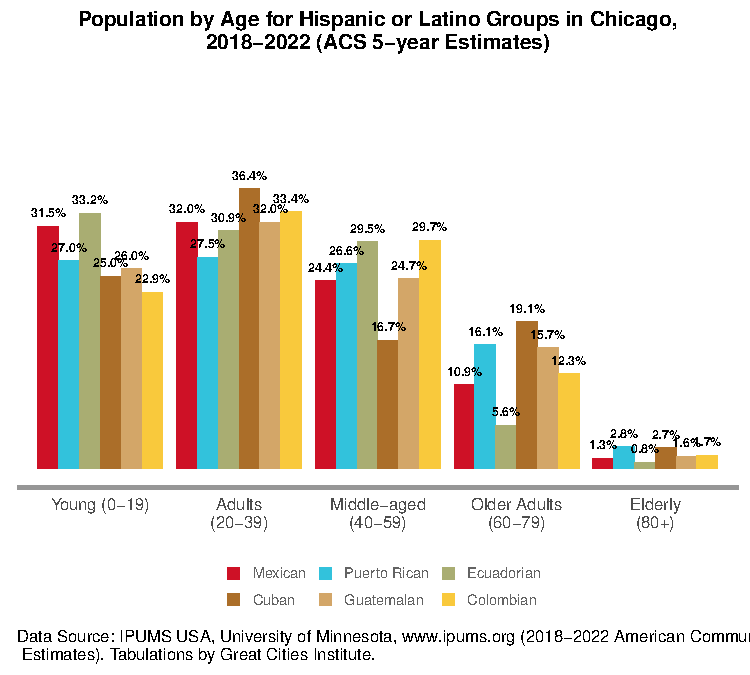
\includegraphics{combined_collar_county_10_files/figure-latex/unnamed-chunk-15-1.pdf}

\includegraphics{combined_collar_county_10_files/figure-latex/unnamed-chunk-16-1.pdf}

\includegraphics{combined_collar_county_10_files/figure-latex/unnamed-chunk-17-1.pdf}

\begin{table}[H]
\centering
\begin{threeparttable}
\caption{\label{tab:unnamed-chunk-20}Total, Hispanic or Latino, and Mexican Population by 10 Community Areas with the Largest Share of Mexican Population, 2018-2022 (ACS 5-year Estimates)}
\centering
\fontsize{8}{10}\selectfont
\begin{tabular}[t]{>{\raggedright\arraybackslash}p{10em}>{\raggedleft\arraybackslash}p{6em}>{\raggedleft\arraybackslash}p{6em}>{\raggedleft\arraybackslash}p{6em}>{\raggedleft\arraybackslash}p{6em}>{\raggedleft\arraybackslash}p{6em}}
\toprule
\multicolumn{1}{>{\centering\arraybackslash}p{10em}}{\begingroup\fontsize{8}{10}\selectfont \textbf{Total of 10 Community Areas}\endgroup} & \multicolumn{1}{>{\centering\arraybackslash}p{6em}}{\begingroup\fontsize{8}{10}\selectfont \textbf{Total Population}\endgroup} & \multicolumn{1}{>{\centering\arraybackslash}p{6em}}{\begingroup\fontsize{8}{10}\selectfont \textbf{Hispanic or Latino Population}\endgroup} & \multicolumn{1}{>{\centering\arraybackslash}p{6em}}{\begingroup\fontsize{8}{10}\selectfont \textbf{Mexican Population}\endgroup} & \multicolumn{1}{>{\centering\arraybackslash}p{6em}}{\begingroup\fontsize{8}{10}\selectfont \textbf{\% Mexicans of Hispanic or Latino}\endgroup} & \multicolumn{1}{>{\centering\arraybackslash}p{6em}}{\begingroup\fontsize{8}{10}\selectfont \textbf{\% Mexicans of Total Population}\endgroup}\\
\midrule
Gage Park & 34,788 & 32,117 & 29,245 & 91.1\% & 84.1\%\\
East Side & 23,942 & 20,791 & 18,901 & 90.9\% & 78.9\%\\
West Lawn & 32,594 & 27,397 & 25,269 & 92.2\% & 77.5\%\\
South Lawndale & 69,708 & 57,024 & 53,315 & 93.5\% & 76.5\%\\
West Elsdon & 18,366 & 14,917 & 13,885 & 93.1\% & 75.6\%\\
Archer Heights & 13,867 & 11,089 & 10,467 & 94.4\% & 75.5\%\\
Brighton Park & 42,243 & 33,789 & 30,269 & 89.6\% & 71.7\%\\
Lower West Side & 34,237 & 23,826 & 21,524 & 90.3\% & 62.9\%\\
New City & 41,048 & 27,426 & 24,431 & 89.1\% & 59.5\%\\
Clearing & 24,728 & 14,882 & 13,403 & 90.1\% & 54.2\%\\
\midrule
\begingroup\fontsize{8}{10}\selectfont \cellcolor{}{\textbf{10 Community Areas with the Largest Share of Mexican Population}}\endgroup & \begingroup\fontsize{8}{10}\selectfont \cellcolor{}{\textbf{335,521}}\endgroup & \begingroup\fontsize{8}{10}\selectfont \cellcolor{}{\textbf{263,258}}\endgroup & \begingroup\fontsize{8}{10}\selectfont \cellcolor{}{\textbf{240,709}}\endgroup & \begingroup\fontsize{8}{10}\selectfont \cellcolor{}{\textbf{91.4\%}}\endgroup & \begingroup\fontsize{8}{10}\selectfont \cellcolor{}{\textbf{71.7\%}}\endgroup\\
\begingroup\fontsize{8}{10}\selectfont \cellcolor{}{\textbf{Other Community Areas}}\endgroup & \begingroup\fontsize{8}{10}\selectfont \cellcolor{}{\textbf{2,374,584}}\endgroup & \begingroup\fontsize{8}{10}\selectfont \cellcolor{}{\textbf{523,792}}\endgroup & \begingroup\fontsize{8}{10}\selectfont \cellcolor{}{\textbf{340,667}}\endgroup & \begingroup\fontsize{8}{10}\selectfont \cellcolor{}{\textbf{65.0\%}}\endgroup & \begingroup\fontsize{8}{10}\selectfont \cellcolor{}{\textbf{14.3\%}}\endgroup\\
\begingroup\fontsize{8}{10}\selectfont \cellcolor{}{\textbf{Chicago}}\endgroup & \begingroup\fontsize{8}{10}\selectfont \cellcolor{}{\textbf{2,710,105}}\endgroup & \begingroup\fontsize{8}{10}\selectfont \cellcolor{}{\textbf{787,050}}\endgroup & \begingroup\fontsize{8}{10}\selectfont \cellcolor{}{\textbf{581,376}}\endgroup & \begingroup\fontsize{8}{10}\selectfont \cellcolor{}{\textbf{73.9\%}}\endgroup & \begingroup\fontsize{8}{10}\selectfont \cellcolor{}{\textbf{21.5\%}}\endgroup\\
\bottomrule
\end{tabular}
\begin{tablenotes}
\small
\item [] \footnotesize{Data Source: IPUMS NHGIS, University of Minnesota, www.nhgis.org (2018-2022 American Community Survey 5-year Estimates). Tabulations by Great Cities Institute.}
\end{tablenotes}
\end{threeparttable}
\end{table}

\begin{table}[H]
\centering
\begin{threeparttable}
\caption{\label{tab:unnamed-chunk-22}Median Age for Mexicans and Other Racial/Ethnic Groups in Chicago, 2018-2022 (ACS 5-year Estimates)}
\centering
\fontsize{8}{10}\selectfont
\begin{tabular}[t]{>{\raggedright\arraybackslash}p{14.2em}>{\raggedleft\arraybackslash}p{15.8em}}
\toprule
\begingroup\fontsize{8}{10}\selectfont \textbf{Race/Ethnicity}\endgroup & \begingroup\fontsize{8}{10}\selectfont \textbf{Median Age}\endgroup\\
\midrule
Mexican & 30\\
Other Hispanics or Latinos & 34\\
White (non-Hispanic or Latino) & 37\\
Black (non-Hispanic or Latino) & 37\\
Other (non-Hispanic or Latino) & 33\\
\bottomrule
\end{tabular}
\begin{tablenotes}
\small
\item [] \footnotesize{Data Source: IPUMS USA, University of Minnesota, www.ipums.org (2018-2022 American Community Survey 5-year Estimates). Tabulations by Great Cities Institute.}
\end{tablenotes}
\end{threeparttable}
\end{table}

\begin{table}[H]
\centering
\begin{threeparttable}
\caption{\label{tab:unnamed-chunk-24}Population by Age for Mexicans and Other Racial/Ethnic Groups in Chicago, 2018-2022 (ACS 5-year Estimates)}
\centering
\fontsize{8}{10}\selectfont
\begin{tabular}[t]{>{\raggedright\arraybackslash}p{10em}>{\raggedleft\arraybackslash}p{3em}>{\raggedleft\arraybackslash}p{3em}>{\raggedleft\arraybackslash}p{3em}>{\raggedleft\arraybackslash}p{3em}>{\raggedleft\arraybackslash}p{3em}>{\raggedleft\arraybackslash}p{3em}>{\raggedleft\arraybackslash}p{3em}>{\raggedleft\arraybackslash}p{3em}>{\raggedleft\arraybackslash}p{3em}>{\raggedleft\arraybackslash}p{3em}}
\toprule
\multicolumn{1}{l}{\bgroup\fontsize{8}{10}\selectfont \textbf{Age Group}\egroup{}} & \multicolumn{2}{c}{\bgroup\fontsize{8}{10}\selectfont \textbf{Mexican}\egroup{}} & \multicolumn{2}{c}{\bgroup\fontsize{8}{10}\selectfont \textbf{\makecell[c]{Other Hispanics\\ or Latinos}}\egroup{}} & \multicolumn{2}{c}{\bgroup\fontsize{8}{10}\selectfont \textbf{\makecell[c]{White\\ (non-Hispanic\\ or Latino)}}\egroup{}} & \multicolumn{2}{c}{\bgroup\fontsize{8}{10}\selectfont \textbf{\makecell[c]{Black\\ (non-Hispanic\\ or Latino)}}\egroup{}} & \multicolumn{2}{c}{\bgroup\fontsize{8}{10}\selectfont \textbf{\makecell[c]{Other\\ (non-Hispanic\\ or Latino)}}\egroup{}} \\
\cmidrule(l{3pt}r{3pt}){1-1} \cmidrule(l{3pt}r{3pt}){2-3} \cmidrule(l{3pt}r{3pt}){4-5} \cmidrule(l{3pt}r{3pt}){6-7} \cmidrule(l{3pt}r{3pt}){8-9} \cmidrule(l{3pt}r{3pt}){10-11}
\multicolumn{1}{>{}p{10em}}{} & \multicolumn{1}{>{}p{3em}}{Number} & \multicolumn{1}{>{}p{3em}}{Percent} & \multicolumn{1}{>{}p{3em}}{Number} & \multicolumn{1}{>{}p{3em}}{Percent} & \multicolumn{1}{>{}p{3em}}{Number} & \multicolumn{1}{>{}p{3em}}{Percent} & \multicolumn{1}{>{}p{3em}}{Number} & \multicolumn{1}{>{}p{3em}}{Percent} & \multicolumn{1}{>{}p{3em}}{Number} & \multicolumn{1}{>{}p{3em}}{Percent}\\
\midrule
Young (0-19) & 163,048 & 31.5\% & 51,591 & 26.8\% & 112,854 & 14.5\% & 166,419 & 24.3\% & 50,607 & 21.3\%\\
Adults (20-39) & 165,753 & 32.0\% & 61,525 & 31.9\% & 308,923 & 39.6\% & 195,130 & 28.5\% & 93,821 & 39.6\%\\
Middle-aged (40-59) & 126,500 & 24.4\% & 49,939 & 25.9\% & 187,649 & 24.1\% & 167,834 & 24.5\% & 53,549 & 22.6\%\\
Older Adults (60-79) & 56,446 & 10.9\% & 25,476 & 13.2\% & 138,641 & 17.8\% & 129,827 & 19.0\% & 31,963 & 13.5\%\\
Elderly (80+) & 6,498 & 1.3\% & 4,109 & 2.1\% & 31,139 & 4.0\% & 25,832 & 3.8\% & 7,256 & 3.1\%\\
\bottomrule
\end{tabular}
\begin{tablenotes}
\small
\item [] \footnotesize{Data Source: IPUMS USA, University of Minnesota, www.ipums.org (2018-2022 American Community Survey 5-year Estimates). Tabulations by Great Cities Institute.}
\end{tablenotes}
\end{threeparttable}
\end{table}

\begin{center}\includegraphics{combined_collar_county_10_files/figure-latex/unnamed-chunk-25-1} \end{center}

\begin{table}[H]
\centering
\begin{threeparttable}
\caption{\label{tab:unnamed-chunk-27}Population by Age for Hispanic or Latino Groups in Chicago, 2018-2022 (ACS 5-year Estimates)}
\centering
\fontsize{8}{10}\selectfont
\begin{tabular}[t]{>{\raggedright\arraybackslash}p{10em}>{\raggedleft\arraybackslash}p{2.5em}>{\raggedleft\arraybackslash}p{2.5em}>{\raggedleft\arraybackslash}p{2.5em}>{\raggedleft\arraybackslash}p{2.5em}>{\raggedleft\arraybackslash}p{2.5em}>{\raggedleft\arraybackslash}p{2.5em}>{\raggedleft\arraybackslash}p{2.5em}>{\raggedleft\arraybackslash}p{2.5em}>{\raggedleft\arraybackslash}p{2.5em}>{\raggedleft\arraybackslash}p{2.5em}>{\raggedleft\arraybackslash}p{2.5em}>{\raggedleft\arraybackslash}p{2.5em}}
\toprule
\multicolumn{1}{l}{\bgroup\fontsize{7.5}{9.5}\selectfont \textbf{Age Group}\egroup{}} & \multicolumn{2}{c}{\bgroup\fontsize{7.5}{9.5}\selectfont \textbf{Mexican}\egroup{}} & \multicolumn{2}{c}{\bgroup\fontsize{7.5}{9.5}\selectfont \textbf{Puerto Rican}\egroup{}} & \multicolumn{2}{c}{\bgroup\fontsize{7.5}{9.5}\selectfont \textbf{Ecuadorian}\egroup{}} & \multicolumn{2}{c}{\bgroup\fontsize{7.5}{9.5}\selectfont \textbf{Cuban}\egroup{}} & \multicolumn{2}{c}{\bgroup\fontsize{7.5}{9.5}\selectfont \textbf{Guatemalan}\egroup{}} & \multicolumn{2}{c}{\bgroup\fontsize{7.5}{9.5}\selectfont \textbf{Colombian}\egroup{}} \\
\cmidrule(l{3pt}r{3pt}){1-1} \cmidrule(l{3pt}r{3pt}){2-3} \cmidrule(l{3pt}r{3pt}){4-5} \cmidrule(l{3pt}r{3pt}){6-7} \cmidrule(l{3pt}r{3pt}){8-9} \cmidrule(l{3pt}r{3pt}){10-11} \cmidrule(l{3pt}r{3pt}){12-13}
\multicolumn{1}{>{}p{10em}}{\begingroup\fontsize{7.5}{9.5}\selectfont \endgroup} & \multicolumn{1}{>{}p{2.5em}}{\begingroup\fontsize{7.5}{9.5}\selectfont Number\endgroup} & \multicolumn{1}{>{}p{2.5em}}{\begingroup\fontsize{7.5}{9.5}\selectfont Percent\endgroup} & \multicolumn{1}{>{}p{2.5em}}{\begingroup\fontsize{7.5}{9.5}\selectfont Number\endgroup} & \multicolumn{1}{>{}p{2.5em}}{\begingroup\fontsize{7.5}{9.5}\selectfont Percent\endgroup} & \multicolumn{1}{>{}p{2.5em}}{\begingroup\fontsize{7.5}{9.5}\selectfont Number\endgroup} & \multicolumn{1}{>{}p{2.5em}}{\begingroup\fontsize{7.5}{9.5}\selectfont Percent\endgroup} & \multicolumn{1}{>{}p{2.5em}}{\begingroup\fontsize{7.5}{9.5}\selectfont Number\endgroup} & \multicolumn{1}{>{}p{2.5em}}{\begingroup\fontsize{7.5}{9.5}\selectfont Percent\endgroup} & \multicolumn{1}{>{}p{2.5em}}{\begingroup\fontsize{7.5}{9.5}\selectfont Number\endgroup} & \multicolumn{1}{>{}p{2.5em}}{\begingroup\fontsize{7.5}{9.5}\selectfont Percent\endgroup} & \multicolumn{1}{>{}p{2.5em}}{\begingroup\fontsize{7.5}{9.5}\selectfont Number\endgroup} & \multicolumn{1}{>{}p{2.5em}}{\begingroup\fontsize{7.5}{9.5}\selectfont Percent\endgroup}\\
\midrule
Young (0-19) & 163,048 & 31.5\% & 23,231 & 27.0\% & 6,812 & 33.2\% & 2,097 & 25.0\% & 4,622 & 26.0\% & 2,330 & 22.9\%\\
Adults (20-39) & 165,753 & 32.0\% & 23,604 & 27.5\% & 6,335 & 30.9\% & 3,053 & 36.4\% & 5,691 & 32.0\% & 3,397 & 33.4\%\\
Middle-aged (40-59) & 126,500 & 24.4\% & 22,838 & 26.6\% & 6,059 & 29.5\% & 1,399 & 16.7\% & 4,389 & 24.7\% & 3,027 & 29.7\%\\
Older Adults (60-79) & 56,446 & 10.9\% & 13,842 & 16.1\% & 1,149 & 5.6\% & 1,602 & 19.1\% & 2,787 & 15.7\% & 1,255 & 12.3\%\\
Elderly (80+) & 6,498 & 1.3\% & 2,393 & 2.8\% & 174 & 0.8\% & 230 & 2.7\% & 279 & 1.6\% & 175 & 1.7\%\\
\bottomrule
\end{tabular}
\begin{tablenotes}
\small
\item [] \footnotesize{Data Source: IPUMS USA, University of Minnesota, www.ipums.org (2018-2022 American Community Survey 5-year Estimates). Tabulations by Great Cities Institute.}
\end{tablenotes}
\end{threeparttable}
\end{table}

\begin{center}\includegraphics{combined_collar_county_10_files/figure-latex/unnamed-chunk-28-1} \end{center}

\begin{table}[H]
\centering
\begin{threeparttable}
\caption{\label{tab:unnamed-chunk-30}Mean Household Size for Mexicans and Other Racial/Ethnic Groups in Chicago, 2018-2022 (ACS 5-year Estimates)}
\centering
\fontsize{8}{10}\selectfont
\begin{tabular}[t]{>{\raggedright\arraybackslash}p{14.2em}>{\raggedleft\arraybackslash}p{15.8em}}
\toprule
\begingroup\fontsize{8}{10}\selectfont \textbf{Race/Ethnicity}\endgroup & \begingroup\fontsize{8}{10}\selectfont \textbf{Mean Household Size}\endgroup\\
\midrule
Mexican & 4.2\\
Other Hispanics or Latinos & 3.4\\
White (non-Hispanic or Latino) & 2.6\\
Black (non-Hispanic or Latino) & 3.0\\
Other (non-Hispanic or Latino) & 3.1\\
\bottomrule
\end{tabular}
\begin{tablenotes}
\small
\item [] \footnotesize{Data Source: IPUMS USA, University of Minnesota, www.ipums.org (2018-2022 American Community Survey 5-year Estimates). Tabulations by Great Cities Institute.}
\end{tablenotes}
\end{threeparttable}
\end{table}

\begin{table}[H]
\centering
\begin{threeparttable}
\caption{\label{tab:unnamed-chunk-32}Mean and Median Household Income for Mexicans and Other Racial/Ethnic Groups in Chicago, 2018-2022 (ACS 5-year Estimates)}
\centering
\fontsize{8}{10}\selectfont
\begin{tabular}[t]{>{\raggedright\arraybackslash}p{14.2em}>{\raggedleft\arraybackslash}p{7.9em}>{\raggedleft\arraybackslash}p{7.9em}}
\toprule
\multicolumn{1}{>{\centering\arraybackslash}p{14.2em}}{\begingroup\fontsize{8}{10}\selectfont \textbf{Race/Ethnicity}\endgroup} & \multicolumn{1}{>{\centering\arraybackslash}p{7.9em}}{\begingroup\fontsize{8}{10}\selectfont \textbf{Mean Household Income}\endgroup} & \multicolumn{1}{>{\centering\arraybackslash}p{7.9em}}{\begingroup\fontsize{8}{10}\selectfont \textbf{Median Household Income}\endgroup}\\
\midrule
Mexican & \$ 77,711 & \$ 63,129\\
Other Hispanics or Latinos & \$ 83,857 & \$ 62,693\\
White (non-Hispanic or Latino) & \$146,895 & \$105,215\\
Black (non-Hispanic or Latino) & \$ 61,498 & \$ 45,326\\
Other (non-Hispanic or Latino) & \$123,052 & \$ 84,986\\
\bottomrule
\end{tabular}
\begin{tablenotes}
\small
\item [] \footnotesize{Data Source: IPUMS USA, University of Minnesota, www.ipums.org (2018-2022 American Community Survey 5-year Estimates). Tabulations by Great Cities Institute.}
\end{tablenotes}
\end{threeparttable}
\end{table}

\begin{table}[H]
\centering
\begin{threeparttable}
\caption{\label{tab:unnamed-chunk-34}Mean and Median Income of Full-time Workers for Mexicans and Other Racial/Ethnic Groups in Chicago, 2018-2022 (ACS 5-year Estimates)}
\centering
\fontsize{8}{10}\selectfont
\begin{tabular}[t]{>{\raggedright\arraybackslash}p{14.2em}>{\raggedleft\arraybackslash}p{7.9em}>{\raggedleft\arraybackslash}p{7.9em}}
\toprule
\begingroup\fontsize{8}{10}\selectfont \textbf{Race/Ethnicity}\endgroup & \begingroup\fontsize{8}{10}\selectfont \textbf{Mean Income}\endgroup & \begingroup\fontsize{8}{10}\selectfont \textbf{Median Income}\endgroup\\
\midrule
Mexican & \$ 52,325 & \$43,236\\
Other Hispanics or Latinos & \$ 65,758 & \$50,000\\
White (non-Hispanic or Latino) & \$114,314 & \$82,672\\
Black (non-Hispanic or Latino) & \$ 60,763 & \$48,136\\
Other (non-Hispanic or Latino) & \$102,800 & \$74,863\\
\bottomrule
\end{tabular}
\begin{tablenotes}
\small
\item [] \footnotesize{Note: Data covers full-time employees working a minimum of 35 hours per week for at least 48 weeks each year.}
\item [] \footnotesize{Data Source: IPUMS USA, University of Minnesota, www.ipums.org (2018-2022 American Community Survey 5-year Estimates). Tabulations by Great Cities Institute.}
\end{tablenotes}
\end{threeparttable}
\end{table}

\begin{table}[H]
\centering
\begin{threeparttable}
\caption{\label{tab:unnamed-chunk-36}Mean and Median Income of Full-time Workers for Hispanic or Latino Groups in Chicago, 2018-2022 (ACS 5-year Estimates)}
\centering
\fontsize{8}{10}\selectfont
\begin{tabular}[t]{>{\raggedright\arraybackslash}p{14.2em}>{\raggedleft\arraybackslash}p{7.9em}>{\raggedleft\arraybackslash}p{7.9em}}
\toprule
\begingroup\fontsize{8}{10}\selectfont \textbf{Race/Ethnicity}\endgroup & \begingroup\fontsize{8}{10}\selectfont \textbf{Mean Income}\endgroup & \begingroup\fontsize{8}{10}\selectfont \textbf{Median Income}\endgroup\\
\midrule
Mexican & \$52,325 & \$43,236\\
Puerto Rican & \$62,228 & \$50,000\\
Ecuadorian & \$46,107 & \$39,924\\
Cuban & \$93,480 & \$62,757\\
Guatemalan & \$48,215 & \$40,000\\
Colombian & \$71,578 & \$54,046\\
\bottomrule
\end{tabular}
\begin{tablenotes}
\small
\item [] \footnotesize{Note: Data covers full-time employees working a minimum of 35 hours per week for at least 48 weeks each year.}
\item [] \footnotesize{Data Source: IPUMS USA, University of Minnesota, www.ipums.org (2018-2022 American Community Survey 5-year Estimates). Tabulations by Great Cities Institute.}
\end{tablenotes}
\end{threeparttable}
\end{table}

\begin{table}[H]
\centering
\begin{threeparttable}
\caption{\label{tab:unnamed-chunk-38}Mean and Median Income of Full-time Workers for Mexico Born and U.S. Born Mexicans in Chicago, 2018-2022 (ACS 5-year Estimates)}
\centering
\fontsize{8}{10}\selectfont
\begin{tabular}[t]{>{\raggedright\arraybackslash}p{14.2em}>{\raggedleft\arraybackslash}p{7.9em}>{\raggedleft\arraybackslash}p{7.9em}}
\toprule
\begingroup\fontsize{8}{10}\selectfont \textbf{Mexican Nativity}\endgroup & \begingroup\fontsize{8}{10}\selectfont \textbf{Mean Income}\endgroup & \begingroup\fontsize{8}{10}\selectfont \textbf{Median Income}\endgroup\\
\midrule
Mexico Born & \$47,238 & \$39,994\\
U.S. Born & \$56,928 & \$45,929\\
\bottomrule
\end{tabular}
\begin{tablenotes}
\small
\item [] \footnotesize{Note: Data covers full-time employees working a minimum of 35 hours per week for at least 48 weeks each year.}
\item [] \footnotesize{Data Source: IPUMS USA, University of Minnesota, www.ipums.org (2018-2022 American Community Survey 5-year Estimates). Tabulations by Great Cities Institute.}
\end{tablenotes}
\end{threeparttable}
\end{table}

\begin{table}[H]
\centering
\begin{threeparttable}
\caption{\label{tab:unnamed-chunk-40}Population in Poverty and Poverty Rate for Mexicans and Other Racial/Ethnic Groups in Chicago, 2000 (Decennial Census), 2008-2012, and 2018-2022 (ACS 5-year Estimates)}
\centering
\fontsize{8}{10}\selectfont
\begin{tabular}[t]{>{\raggedright\arraybackslash}p{14.2em}>{\raggedleft\arraybackslash}p{3.68em}>{\raggedleft\arraybackslash}p{3.68em}>{\raggedleft\arraybackslash}p{3.68em}>{\raggedleft\arraybackslash}p{3.68em}>{\raggedleft\arraybackslash}p{3.68em}>{\raggedleft\arraybackslash}p{3.68em}>{\raggedleft\arraybackslash}p{3.68em}}
\toprule
\multicolumn{1}{l}{\bgroup\fontsize{8}{10}\selectfont \textbf{Race/Ethnicity}\egroup{}} & \multicolumn{2}{c}{\bgroup\fontsize{8}{10}\selectfont \textbf{\makecell[c]{Poverty\\in 2000 }}\egroup{}} & \multicolumn{2}{c}{\bgroup\fontsize{8}{10}\selectfont \textbf{\makecell[c]{Poverty\\in 2008-2012 }}\egroup{}} & \multicolumn{2}{c}{\bgroup\fontsize{8}{10}\selectfont \textbf{\makecell[c]{Poverty\\in 2018-2022}}\egroup{}} & \multicolumn{1}{c}{\bgroup\fontsize{8}{10}\selectfont \textbf{\makecell[c]{Changes\\from 2000\\to 2018-2022}}\egroup{}} \\
\cmidrule(l{3pt}r{3pt}){1-1} \cmidrule(l{3pt}r{3pt}){2-3} \cmidrule(l{3pt}r{3pt}){4-5} \cmidrule(l{3pt}r{3pt}){6-7} \cmidrule(l{3pt}r{3pt}){8-8}
\multicolumn{1}{>{\centering\arraybackslash}p{14.2em}}{\begingroup\fontsize{8}{10}\selectfont \endgroup} & \multicolumn{1}{>{\centering\arraybackslash}p{3.68em}}{\begingroup\fontsize{8}{10}\selectfont Number\endgroup} & \multicolumn{1}{>{\centering\arraybackslash}p{3.68em}}{\begingroup\fontsize{8}{10}\selectfont Percent\endgroup} & \multicolumn{1}{>{\centering\arraybackslash}p{3.68em}}{\begingroup\fontsize{8}{10}\selectfont Number\endgroup} & \multicolumn{1}{>{\centering\arraybackslash}p{3.68em}}{\begingroup\fontsize{8}{10}\selectfont Percent\endgroup} & \multicolumn{1}{>{\centering\arraybackslash}p{3.68em}}{\begingroup\fontsize{8}{10}\selectfont Number\endgroup} & \multicolumn{1}{>{\centering\arraybackslash}p{3.68em}}{\begingroup\fontsize{8}{10}\selectfont Percent\endgroup} & \multicolumn{1}{>{\centering\arraybackslash}p{3.68em}}{\begingroup\fontsize{8}{10}\selectfont Difference\endgroup}\\
\midrule
Mexican & 102,180 & 18.8\% & 115,240 & 22.6\% & 80,224 & 15.5\% & -3.4\%\\
Other Hispanics or Latinos & 45,249 & 21.4\% & 30,839 & 20.0\% & 30,103 & 15.6\% & -5.7\%\\
White (non-Hispanic or Latino) & 90,160 & 9.9\% & 92,174 & 12.1\% & 78,923 & 10.1\% & 0.2\%\\
Black (non-Hispanic or Latino) & 325,923 & 30.4\% & 276,940 & 33.0\% & 186,352 & 27.2\% & -3.2\%\\
Other (non-Hispanic or Latino) & 34,278 & 18.9\% & 36,859 & 20.7\% & 41,455 & 17.5\% & -1.4\%\\
\bottomrule
\end{tabular}
\begin{tablenotes}
\small
\item [] \footnotesize{Data Source: IPUMS USA, University of Minnesota, www.ipums.org (2000 Decennial Census, 2018-2012, and 2018-2022 American Community Survey 5-year Estimates). Tabulations by Great Cities Institute.}
\end{tablenotes}
\end{threeparttable}
\end{table}

\clearpage

\section{Education}\label{education}

\begin{table}[H]
\centering
\begin{threeparttable}
\caption{\label{tab:unnamed-chunk-42}Number and Percent in Public and Private Schools for Mexicans and Other Racial/Ethnic Groups in Chicago, 2018-2022 (ACS 5-year Estimates)}
\centering
\fontsize{8}{10}\selectfont
\begin{tabular}[t]{>{\raggedright\arraybackslash}p{10em}>{\raggedleft\arraybackslash}p{3em}>{\raggedleft\arraybackslash}p{3em}>{\raggedleft\arraybackslash}p{3em}>{\raggedleft\arraybackslash}p{3em}>{\raggedleft\arraybackslash}p{3em}>{\raggedleft\arraybackslash}p{3em}>{\raggedleft\arraybackslash}p{3em}>{\raggedleft\arraybackslash}p{3em}>{\raggedleft\arraybackslash}p{3em}>{\raggedleft\arraybackslash}p{3em}}
\toprule
\multicolumn{1}{l}{\bgroup\fontsize{8}{10}\selectfont \textbf{Age Group}\egroup{}} & \multicolumn{2}{c}{\bgroup\fontsize{8}{10}\selectfont \textbf{Mexican}\egroup{}} & \multicolumn{2}{c}{\bgroup\fontsize{8}{10}\selectfont \textbf{\makecell[c]{Other Hispanics\\ or Latinos}}\egroup{}} & \multicolumn{2}{c}{\bgroup\fontsize{8}{10}\selectfont \textbf{\makecell[c]{White\\ (non-Hispanic\\ or Latino)}}\egroup{}} & \multicolumn{2}{c}{\bgroup\fontsize{8}{10}\selectfont \textbf{\makecell[c]{Black\\ (non-Hispanic\\ or Latino)}}\egroup{}} & \multicolumn{2}{c}{\bgroup\fontsize{8}{10}\selectfont \textbf{\makecell[c]{Other\\ (non-Hispanic\\ or Latino)}}\egroup{}} \\
\cmidrule(l{3pt}r{3pt}){1-1} \cmidrule(l{3pt}r{3pt}){2-3} \cmidrule(l{3pt}r{3pt}){4-5} \cmidrule(l{3pt}r{3pt}){6-7} \cmidrule(l{3pt}r{3pt}){8-9} \cmidrule(l{3pt}r{3pt}){10-11}
\multicolumn{1}{>{}p{10em}}{} & \multicolumn{1}{>{}p{3em}}{Number} & \multicolumn{1}{>{}p{3em}}{Percent} & \multicolumn{1}{>{}p{3em}}{Number} & \multicolumn{1}{>{}p{3em}}{Percent} & \multicolumn{1}{>{}p{3em}}{Number} & \multicolumn{1}{>{}p{3em}}{Percent} & \multicolumn{1}{>{}p{3em}}{Number} & \multicolumn{1}{>{}p{3em}}{Percent} & \multicolumn{1}{>{}p{3em}}{Number} & \multicolumn{1}{>{}p{3em}}{Percent}\\
\midrule
Public & 131,597 & 86.0\% & 40,463 & 76.8\% & 65,331 & 47.4\% & 130,402 & 81.9\% & 36,563 & 58.3\%\\
Private & 21,366 & 14.0\% & 12,189 & 23.2\% & 72,490 & 52.6\% & 28,883 & 18.1\% & 26,199 & 41.7\%\\
\bottomrule
\end{tabular}
\begin{tablenotes}
\small
\item [] \footnotesize{Data Source: IPUMS USA, University of Minnesota, www.ipums.org (2018-2022 American Community Survey 5-year Estimates). Tabulations by Great Cities Institute.}
\end{tablenotes}
\end{threeparttable}
\end{table}

\begin{table}[H]
\centering
\begin{threeparttable}
\caption{\label{tab:unnamed-chunk-44}Performance in Chicago Public Schools (CPS) Elementary Schools in Four Community Areas with Largest Share of Mexican Population and Performance Citywide by Race/Ethnicity, 2023}
\centering
\fontsize{8}{10}\selectfont
\begin{tabular}[t]{>{\raggedright\arraybackslash}p{18.2em}>{\raggedleft\arraybackslash}p{7.26em}>{\raggedleft\arraybackslash}p{7.26em}>{\raggedleft\arraybackslash}p{7.26em}}
\toprule
\multicolumn{1}{l}{\bgroup\fontsize{8}{10}\selectfont \textbf{Aggregation}\egroup{}} & \multicolumn{1}{c}{\bgroup\fontsize{8}{10}\selectfont \textbf{\makecell[c]{Mean English\\Language Arts\\Proficiency}}\egroup{}} & \multicolumn{1}{c}{\bgroup\fontsize{8}{10}\selectfont \textbf{\makecell[c]{Mean Math\\Proficiency}}\egroup{}} & \multicolumn{1}{c}{\bgroup\fontsize{8}{10}\selectfont \textbf{\makecell[c]{Mean Science\\Proficiency}}\egroup{}} \\
\cmidrule(l{3pt}r{3pt}){1-1} \cmidrule(l{3pt}r{3pt}){2-2} \cmidrule(l{3pt}r{3pt}){3-3} \cmidrule(l{3pt}r{3pt}){4-4}
\multicolumn{1}{>{\centering\arraybackslash}p{18.2em}}{} & \multicolumn{1}{>{\centering\arraybackslash}p{7.26em}}{Percent} & \multicolumn{1}{>{\centering\arraybackslash}p{7.26em}}{Percent} & \multicolumn{1}{>{\centering\arraybackslash}p{7.26em}}{Percent}\\
\midrule
Mean Metrics for Hispanic or Latino Students in Four Community Areas with Largest Share of Mexican Population & 19.4\% & 11.9\% & 36.7\%\\
Total CPS Hispanic or Latino Students & 21.2\% & 13.6\% & 35.6\%\\
Total CPS White (non-Hispanic or Latino) Students & 54.3\% & 48.4\% & 65.0\%\\
Total CPS Black (non-Hispanic or Latino) Students & 16.5\% & 8.1\% & 24.4\%\\
Total CPS Other (non-Hispanic or Latino) Students & 47.7\% & 41.0\% & 57.0\%\\
\bottomrule
\end{tabular}
\begin{tablenotes}
\small
\item [] \footnotesize{Sample size: 31 Chicago Public Schools Elementary Schools in Gage Park, East Side, West Lawn, and South Lawndale.}
\item [] \footnotesize{Data Source: Illinois Report Card (2023). Tabulations by Great Cities Institute.}
\end{tablenotes}
\end{threeparttable}
\end{table}

\begin{table}[H]
\centering
\begin{threeparttable}
\caption{\label{tab:unnamed-chunk-45}Chronic Absenteeism in Chicago Public Schools (CPS) Elementary Schools in Four Community Areas with Largest Share of Mexican Population, 2023}
\centering
\fontsize{8}{10}\selectfont
\begin{tabular}[t]{>{\raggedright\arraybackslash}p{18.2em}>{\raggedleft\arraybackslash}p{11.8em}}
\toprule
\multicolumn{1}{l}{\bgroup\fontsize{8}{10}\selectfont \textbf{Aggregation}\egroup{}} & \multicolumn{1}{c}{\bgroup\fontsize{8}{10}\selectfont \textbf{Mean Chronic Absenteeism}\egroup{}} \\
\cmidrule(l{3pt}r{3pt}){1-1} \cmidrule(l{3pt}r{3pt}){2-2}
\multicolumn{1}{c}{} & \multicolumn{1}{c}{Percent}\\
\midrule
Mean Metrics for Hispanic or Latino Students in Four Community Areas with Largest Share of Mexican Population & 36.2\%\\
Total CPS Hispanic or Latino Students & 40.3\%\\
Total CPS White (non-Hispanic or Latino) Students & 27.1\%\\
Total CPS Black (non-Hispanic or Latino) Students & 45.8\%\\
Total CPS Other (non-Hispanic or Latino) Students & 31.9\%\\
\bottomrule
\end{tabular}
\begin{tablenotes}
\small
\item [] \footnotesize{Note: Sample size: 31 Chicago Public Schools Elementary Schools in Gage Park, East Side, West Lawn, and South Lawndale.}
\item [] \footnotesize{Note: Chronic Absenteeism is defined as students who miss 10 percent or more of school days per year.}
\item [] \footnotesize{Data Source: Illinois Report Card (2023). Tabulations by Great Cities Institute.}
\end{tablenotes}
\end{threeparttable}
\end{table}

\begin{table}[H]
\centering
\begin{threeparttable}
\caption{\label{tab:unnamed-chunk-47}Number and Percent of Population with Limited English Proficiency for Mexicans and Other Racial/Ethnic Groups in Chicago, 2018-2022 (ACS 5-year Estimates)}
\centering
\fontsize{8}{10}\selectfont
\begin{tabular}[t]{>{\raggedright\arraybackslash}p{14.2em}>{\raggedleft\arraybackslash}p{7.9em}>{\raggedleft\arraybackslash}p{7.9em}}
\toprule
\begingroup\fontsize{8}{10}\selectfont \textbf{Race/Ethnicity}\endgroup & \begingroup\fontsize{8}{10}\selectfont \textbf{Number}\endgroup & \begingroup\fontsize{8}{10}\selectfont \textbf{Percent}\endgroup\\
\midrule
Mexican & 89,859 & 17.3\%\\
Other Hispanics or Latinos & 23,729 & 12.3\%\\
White (non-Hispanic or Latino) & 18,629 & 2.4\%\\
Black (non-Hispanic or Latino) & 1,788 & 0.3\%\\
Other (non-Hispanic or Latino) & 26,249 & 11.1\%\\
\bottomrule
\end{tabular}
\begin{tablenotes}
\small
\item [] \footnotesize{Note: English Proficiency is defined as respondents who does not speak English or speaks English poorly.}
\item [] \footnotesize{Data Source: IPUMS USA, University of Minnesota, www.ipums.org (2018-2022 American Community Survey 5-year Estimates). Tabulations by Great Cities Institute.}
\end{tablenotes}
\end{threeparttable}
\end{table}

\begin{table}[H]
\centering
\begin{threeparttable}
\caption{\label{tab:unnamed-chunk-49}Number and Percent of Non-citizens enrolled in Public Schools for Mexicans and Other Racial/Ethnic Groups in Chicago, 2018-2022 (ACS 5-year Estimates)}
\centering
\fontsize{8}{10}\selectfont
\begin{tabular}[t]{>{\raggedright\arraybackslash}p{14.2em}>{\raggedleft\arraybackslash}p{7.9em}>{\raggedleft\arraybackslash}p{7.9em}}
\toprule
\begingroup\fontsize{8}{10}\selectfont \textbf{Race/Ethnicity}\endgroup & \begingroup\fontsize{8}{10}\selectfont \textbf{Number}\endgroup & \begingroup\fontsize{8}{10}\selectfont \textbf{Percent}\endgroup\\
\midrule
Mexican & 5,566 & 3.6\%\\
Other Hispanics or Latinos & 3,112 & 5.9\%\\
White (non-Hispanic or Latino) & 2,844 & 2.1\%\\
Black (non-Hispanic or Latino) & 2,399 & 1.5\%\\
Other (non-Hispanic or Latino) & 5,871 & 9.4\%\\
\bottomrule
\end{tabular}
\begin{tablenotes}
\small
\item [] \footnotesize{Data Source: IPUMS USA, University of Minnesota, www.ipums.org (2018-2022 American Community Survey 5-year Estimates). Tabulations by Great Cities Institute.}
\end{tablenotes}
\end{threeparttable}
\end{table}

\begin{table}[H]
\centering
\begin{threeparttable}
\caption{\label{tab:unnamed-chunk-51}Number and Percent of Population Attending Undergraduate or Graduate Colleges or Professional Schools for Mexicans and Other Racial/Ethnic Groups in Chicago, 2018-2022 (ACS 5-year Estimates)}
\centering
\fontsize{8}{10}\selectfont
\begin{tabular}[t]{>{\raggedright\arraybackslash}p{14.2em}>{\raggedleft\arraybackslash}p{6.45em}>{\raggedleft\arraybackslash}p{6.45em}>{\raggedleft\arraybackslash}p{6.45em}>{\raggedleft\arraybackslash}p{6.45em}}
\toprule
\multicolumn{1}{l}{\bgroup\fontsize{8}{10}\selectfont \textbf{Race/Ethnicity}\egroup{}} & \multicolumn{2}{c}{\bgroup\fontsize{8}{10}\selectfont \textbf{Ages 18-24}\egroup{}} & \multicolumn{2}{c}{\bgroup\fontsize{8}{10}\selectfont \textbf{Ages 25-34}\egroup{}} \\
\cmidrule(l{3pt}r{3pt}){1-1} \cmidrule(l{3pt}r{3pt}){2-3} \cmidrule(l{3pt}r{3pt}){4-5}
\multicolumn{1}{>{\centering\arraybackslash}p{14.2em}}{} & \multicolumn{1}{>{\centering\arraybackslash}p{6.45em}}{Number} & \multicolumn{1}{>{\centering\arraybackslash}p{6.45em}}{Percent} & \multicolumn{1}{>{\centering\arraybackslash}p{6.45em}}{Number} & \multicolumn{1}{>{\centering\arraybackslash}p{6.45em}}{Percent}\\
\midrule
Mexican & 22,705 & 35.7\% & 6,449 & 7.7\%\\
Other Hispanics or Latinos & 7,707 & 39.1\% & 4,435 & 13.8\%\\
White (non-Hispanic or Latino) & 32,987 & 49.3\% & 21,242 & 11.3\%\\
Black (non-Hispanic or Latino) & 16,458 & 25.9\% & 9,301 & 8.8\%\\
Other (non-Hispanic or Latino) & 15,004 & 59.9\% & 11,042 & 20.7\%\\
\bottomrule
\end{tabular}
\begin{tablenotes}
\small
\item [] \footnotesize{Data Source: IPUMS USA, University of Minnesota, www.ipums.org (2018-2022 American Community Survey 5-year Estimates). Tabulations by Great Cities Institute.}
\end{tablenotes}
\end{threeparttable}
\end{table}

\begin{landscape}

\begin{table}[H]
\centering
\begin{threeparttable}
\caption{\label{tab:unnamed-chunk-53}Educational Attainment of Population Aged 25 and over for Mexicans and Other Racial/Ethnic Groups in Chicago, 2018-2022 (ACS 5-year Estimates)}
\centering
\fontsize{8}{10}\selectfont
\begin{tabular}[t]{>{\raggedright\arraybackslash}p{14.2em}>{\raggedleft\arraybackslash}p{4.58em}>{\raggedleft\arraybackslash}p{4.58em}>{\raggedleft\arraybackslash}p{4.58em}>{\raggedleft\arraybackslash}p{4.58em}>{\raggedleft\arraybackslash}p{4.58em}>{\raggedleft\arraybackslash}p{4.58em}>{\raggedleft\arraybackslash}p{4.58em}>{\raggedleft\arraybackslash}p{4.58em}>{\raggedleft\arraybackslash}p{4.58em}>{\raggedleft\arraybackslash}p{4.58em}}
\toprule
\multicolumn{1}{l}{\bgroup\fontsize{8}{10}\selectfont \textbf{Educational Level}\egroup{}} & \multicolumn{2}{c}{\bgroup\fontsize{8}{10}\selectfont \textbf{Mexican}\egroup{}} & \multicolumn{2}{c}{\bgroup\fontsize{8}{10}\selectfont \textbf{\makecell[c]{Other Hispanics\\or Latinos}}\egroup{}} & \multicolumn{2}{c}{\bgroup\fontsize{8}{10}\selectfont \textbf{\makecell[c]{White\\(non-Hispanic or Latino)}}\egroup{}} & \multicolumn{2}{c}{\bgroup\fontsize{8}{10}\selectfont \textbf{\makecell[c]{Black\\(non-Hispanic or Latino)}}\egroup{}} & \multicolumn{2}{c}{\bgroup\fontsize{8}{10}\selectfont \textbf{\makecell[c]{Other\\(non-Hispanic or Latino)}}\egroup{}} \\
\cmidrule(l{3pt}r{3pt}){1-1} \cmidrule(l{3pt}r{3pt}){2-3} \cmidrule(l{3pt}r{3pt}){4-5} \cmidrule(l{3pt}r{3pt}){6-7} \cmidrule(l{3pt}r{3pt}){8-9} \cmidrule(l{3pt}r{3pt}){10-11}
\multicolumn{1}{>{}p{14.2em}}{} & \multicolumn{1}{>{}p{4.58em}}{Number} & \multicolumn{1}{>{}p{4.58em}}{Percent} & \multicolumn{1}{>{}p{4.58em}}{Number} & \multicolumn{1}{>{}p{4.58em}}{Percent} & \multicolumn{1}{>{}p{4.58em}}{Number} & \multicolumn{1}{>{}p{4.58em}}{Percent} & \multicolumn{1}{>{}p{4.58em}}{Number} & \multicolumn{1}{>{}p{4.58em}}{Percent} & \multicolumn{1}{>{}p{4.58em}}{Number} & \multicolumn{1}{>{}p{4.58em}}{Percent}\\
\midrule
No Schooling Completed & 18,404 & 5.9\% & 4,218 & 3.3\% & 4,533 & 0.7\% & 5,511 & 1.2\% & 5,939 & 3.6\%\\
Less than High School & 78,226 & 25.2\% & 21,246 & 16.8\% & 19,874 & 3.2\% & 55,257 & 11.7\% & 14,180 & 8.5\%\\
Regular High School Diploma, GED or Alternative Credential & 101,055 & 32.6\% & 31,877 & 25.2\% & 82,167 & 13.4\% & 133,418 & 28.3\% & 20,228 & 12.2\%\\
Some College, No Degree & 46,070 & 14.9\% & 22,554 & 17.8\% & 73,901 & 12.0\% & 124,818 & 26.5\% & 16,749 & 10.1\%\\
Associate's Degree & 17,726 & 5.7\% & 9,969 & 7.9\% & 25,436 & 4.1\% & 38,312 & 8.1\% & 8,721 & 5.2\%\\
Bachelor's Degree & 34,239 & 11.0\% & 22,432 & 17.7\% & 229,365 & 37.4\% & 65,976 & 14.0\% & 54,042 & 32.5\%\\
Master's Degree or Higher & 14,420 & 4.6\% & 14,261 & 11.3\% & 178,724 & 29.1\% & 48,449 & 10.3\% & 46,394 & 27.9\%\\
\bottomrule
\end{tabular}
\begin{tablenotes}
\small
\item [] \footnotesize{Data Source: IPUMS USA, University of Minnesota, www.ipums.org (2018-2022 American Community Survey 5-year Estimates). Tabulations by Great Cities Institute.}
\end{tablenotes}
\end{threeparttable}
\end{table}

\end{landscape}

\begin{table}[H]
\centering
\begin{threeparttable}
\caption{\label{tab:unnamed-chunk-55}Educational Attainment of Population Aged 25 and over for Mexico Born and U.S. Born Mexicans in Chicago, 2018-2022 (ACS 5-year Estimates)}
\centering
\fontsize{8}{10}\selectfont
\begin{tabular}[t]{>{\raggedright\arraybackslash}p{14.2em}>{\raggedleft\arraybackslash}p{6.45em}>{\raggedleft\arraybackslash}p{6.45em}>{\raggedleft\arraybackslash}p{6.45em}>{\raggedleft\arraybackslash}p{6.45em}}
\toprule
\multicolumn{1}{l}{\bgroup\fontsize{8}{10}\selectfont \textbf{Educational Level}\egroup{}} & \multicolumn{2}{c}{\bgroup\fontsize{8}{10}\selectfont \textbf{\makecell[c]{Mexicans Born\\in Mexico}}\egroup{}} & \multicolumn{2}{c}{\bgroup\fontsize{8}{10}\selectfont \textbf{\makecell[c]{Mexicans Born\\in the U.S.}}\egroup{}} \\
\cmidrule(l{3pt}r{3pt}){1-1} \cmidrule(l{3pt}r{3pt}){2-3} \cmidrule(l{3pt}r{3pt}){4-5}
\multicolumn{1}{>{}p{14.2em}}{} & \multicolumn{1}{>{}p{6.45em}}{Number} & \multicolumn{1}{>{}p{6.45em}}{Percent} & \multicolumn{1}{>{}p{6.45em}}{Number} & \multicolumn{1}{>{}p{6.45em}}{Percent}\\
\midrule
No Schooling Completed & 15,862 & 8.8\% & 2,288 & 1.8\%\\
Less than High School & 63,683 & 35.5\% & 13,410 & 10.6\%\\
Regular High School Diploma, GED or Alternative Credential & 61,816 & 34.4\% & 38,117 & 30.1\%\\
Some College, No Degree & 17,996 & 10.0\% & 27,380 & 21.6\%\\
Associate's Degree & 6,252 & 3.5\% & 11,135 & 8.8\%\\
Bachelor's Degree & 9,525 & 5.3\% & 24,404 & 19.3\%\\
Master's Degree or Higher & 4,353 & 2.4\% & 9,849 & 7.8\%\\
\bottomrule
\end{tabular}
\begin{tablenotes}
\small
\item [] \footnotesize{Data Source: IPUMS USA, University of Minnesota, www.ipums.org (2018-2022 American Community Survey 5-year Estimates). Tabulations by Great Cities Institute.}
\end{tablenotes}
\end{threeparttable}
\end{table}

\begin{center}\includegraphics{combined_collar_county_10_files/figure-latex/unnamed-chunk-57-1} \end{center}

\section{Housing}\label{housing}

\begin{table}[H]
\centering
\begin{threeparttable}
\caption{\label{tab:unnamed-chunk-58}Homeownership for Mexicans and Other Racial/Ethnic Groups in Chicago and the U.S., 2000 (Decennial Census), 2008-2012, and 2018-2022 (ACS 5-year Estimates)}
\centering
\fontsize{8}{10}\selectfont
\begin{tabular}[t]{>{\raggedright\arraybackslash}p{14.2em}>{\raggedleft\arraybackslash}p{3.85em}>{\raggedleft\arraybackslash}p{3.85em}>{\raggedleft\arraybackslash}p{3.85em}>{\raggedleft\arraybackslash}p{3.85em}>{\raggedleft\arraybackslash}p{3.85em}>{\raggedleft\arraybackslash}p{3.85em}>{\raggedleft\arraybackslash}p{3.85em}>{\raggedleft\arraybackslash}p{3.85em}}
\toprule
\multicolumn{1}{l}{\bgroup\fontsize{8}{10}\selectfont \textbf{Race/Ethnicity}\egroup{}} & \multicolumn{2}{c}{\bgroup\fontsize{8}{10}\selectfont \textbf{2000}\egroup{}} & \multicolumn{2}{c}{\bgroup\fontsize{8}{10}\selectfont \textbf{2008-2012}\egroup{}} & \multicolumn{2}{c}{\bgroup\fontsize{8}{10}\selectfont \textbf{2018-2022}\egroup{}} & \multicolumn{2}{c}{\bgroup\fontsize{8}{10}\selectfont \textbf{\makecell[c]{Change from\\2000 to 2018-2022}}\egroup{}} \\
\cmidrule(l{3pt}r{3pt}){1-1} \cmidrule(l{3pt}r{3pt}){2-3} \cmidrule(l{3pt}r{3pt}){4-5} \cmidrule(l{3pt}r{3pt}){6-7} \cmidrule(l{3pt}r{3pt}){8-9}
\multicolumn{1}{>{}p{14.2em}}{} & \multicolumn{1}{>{}p{3.85em}}{Number} & \multicolumn{1}{>{}p{3.85em}}{Percent} & \multicolumn{1}{>{}p{3.85em}}{Number} & \multicolumn{1}{>{}p{3.85em}}{Percent} & \multicolumn{1}{>{}p{3.85em}}{Number} & \multicolumn{1}{>{}p{3.85em}}{Percent} & \multicolumn{1}{>{}p{3.85em}}{Number} & \multicolumn{1}{>{}p{3.85em}}{Percent}\\
\midrule
\addlinespace[0.3em]
\multicolumn{9}{l}{\textbf{Chicago}}\\
\hline
Mexican & 53,008 & 41.2\% & 59,920 & 47.5\% & 74,970 & 49.9\% & 21,962 & 8.8\%\\
Other Hispanics or Latinos & 22,685 & 34.5\% & 19,494 & 39.5\% & 28,701 & 41.7\% & 6,016 & 7.2\%\\
White (non-Hispanic or Latino) & 232,907 & 52.2\% & 210,995 & 56.3\% & 206,780 & 52.7\% & -26,127 & 0.5\%\\
Black (non-Hispanic or Latino) & 133,828 & 37.0\% & 111,882 & 35.8\% & 99,876 & 34.6\% & -33,952 & -2.4\%\\
Other (non-Hispanic or Latino) & 24,087 & 36.7\% & 28,551 & 42.4\% & 44,240 & 45.5\% & 20,153 & 8.8\%\\
\addlinespace[0.3em]
\hline
\multicolumn{9}{l}{\textbf{U.S.}}\\
\hline
Mexican & 2,427,031 & 48.4\% & 3,978,209 & 49.2\% & 5,235,249 & 52.5\% & 2,808,218 & 4.1\%\\
Other Hispanics or Latinos & 1,765,890 & 42.3\% & 2,380,084 & 44.2\% & 3,575,520 & 45.9\% & 1,809,630 & 3.6\%\\
White (non-Hispanic or Latino) & 57,289,023 & 72.4\% & 58,845,290 & 72.6\% & 59,628,210 & 72.7\% & 2,339,187 & 0.2\%\\
Black (non-Hispanic or Latino) & 5,496,423 & 46.6\% & 6,045,479 & 44.5\% & 6,490,005 & 43.0\% & 993,582 & -3.6\%\\
Other (non-Hispanic or Latino) & 2,832,626 & 52.3\% & 3,990,167 & 56.5\% & 6,395,041 & 59.1\% & 3,562,415 & 6.8\%\\
\bottomrule
\end{tabular}
\begin{tablenotes}
\small
\item [] \footnotesize{Data Source: IPUMS USA, University of Minnesota, www.ipums.org (2000 Decennial Census, 2008-2012, and 2018-2022 American Community Survey 5-year Estimates).Tabulations by Great Cities Institute.}
\end{tablenotes}
\end{threeparttable}
\end{table}

\begin{table}[H]
\centering
\begin{threeparttable}
\caption{\label{tab:unnamed-chunk-60}Number and Percent of Households Living in Crowded Housing for Mexicans and Other Racial/Ethnic Groups in Chicago, 2018-2022 (ACS 5-year Estimates)}
\centering
\fontsize{8}{10}\selectfont
\begin{tabular}[t]{>{\raggedright\arraybackslash}p{14.2em}>{\raggedleft\arraybackslash}p{12.9em}>{\raggedleft\arraybackslash}p{12.9em}}
\toprule
\begingroup\fontsize{8}{10}\selectfont \textbf{Race/Ethnicity}\endgroup & \begingroup\fontsize{8}{10}\selectfont \textbf{Number}\endgroup & \begingroup\fontsize{8}{10}\selectfont \textbf{Percent}\endgroup\\
\midrule
Mexican & 12,862 & 8.3\%\\
Other Hispanics or Latinos & 2,343 & 3.3\%\\
White (non-Hispanic or Latino) & 4,790 & 1.2\%\\
Black (non-Hispanic or Latino) & 7,402 & 2.4\%\\
Other (non-Hispanic or Latino) & 6,056 & 6.0\%\\
\bottomrule
\end{tabular}
\begin{tablenotes}
\small
\item [] \footnotesize{Note: Housing is defined as overcrowded if more than one person in the room.}
\item [] \footnotesize{Data Source: IPUMS USA, University of Minnesota, www.ipums.org (2018-2022 American Community Survey 5-year Estimates). Tabulations by Great Cities Institute.}
\end{tablenotes}
\end{threeparttable}
\end{table}

\begin{table}[H]
\centering
\begin{threeparttable}
\caption{\label{tab:unnamed-chunk-61}Number and Percent of Rent Burdened Households for Mexicans and Other Racial/Ethnic Groups in Chicago, 2018-2022 (ACS 5-year Estimates)}
\centering
\fontsize{8}{10}\selectfont
\begin{tabular}[t]{>{\raggedright\arraybackslash}p{14.2em}>{\raggedleft\arraybackslash}p{6.45em}>{\raggedleft\arraybackslash}p{6.45em}>{\raggedleft\arraybackslash}p{6.45em}>{\raggedleft\arraybackslash}p{6.45em}}
\toprule
\multicolumn{1}{l}{\bgroup\fontsize{8}{10}\selectfont \textbf{Race/Ethnicity}\egroup{}} & \multicolumn{2}{c}{\bgroup\fontsize{8}{10}\selectfont \textbf{\makecell[c]{More than 30\% of\\Household Income Spent\\on Rental Costs}}\egroup{}} & \multicolumn{2}{c}{\bgroup\fontsize{8}{10}\selectfont \textbf{\makecell[c]{More than 50\% of\\Household Income Spent\\on Rental Costs}}\egroup{}} \\
\cmidrule(l{3pt}r{3pt}){1-1} \cmidrule(l{3pt}r{3pt}){2-3} \cmidrule(l{3pt}r{3pt}){4-5}
\multicolumn{1}{>{\centering\arraybackslash}p{14.2em}}{} & \multicolumn{1}{>{\centering\arraybackslash}p{6.45em}}{Number} & \multicolumn{1}{>{\centering\arraybackslash}p{6.45em}}{Percent} & \multicolumn{1}{>{\centering\arraybackslash}p{6.45em}}{Number} & \multicolumn{1}{>{\centering\arraybackslash}p{6.45em}}{Percent}\\
\midrule
Mexican & 38,258 & 50.8\% & 17,361 & 23.1\%\\
Other Hispanics or Latinos & 21,655 & 54.0\% & 11,512 & 28.7\%\\
White (non-Hispanic or Latino) & 69,290 & 37.3\% & 33,296 & 17.9\%\\
Black (non-Hispanic or Latino) & 108,343 & 57.4\% & 67,686 & 35.9\%\\
Other (non-Hispanic or Latino) & 22,851 & 43.1\% & 13,816 & 26.1\%\\
\bottomrule
\end{tabular}
\begin{tablenotes}
\small
\item [] \footnotesize{Note: Rent cost burdened households defined as households paying 30 percent or more of household income on rental housing costs.}
\item [] \footnotesize{Data Source: IPUMS USA, University of Minnesota, www.ipums.org (2018-2022 American Community Survey 5-year Estimates). Tabulations by Great Cities Institute.}
\end{tablenotes}
\end{threeparttable}
\end{table}

\begin{table}[H]
\centering
\begin{threeparttable}
\caption{\label{tab:unnamed-chunk-62}Number and Percent of Owner Cost Burdened Households for Mexicans and Other Racial/Ethnic Groups in Chicago, 2018-2022 (ACS 5-year Estimates)}
\centering
\fontsize{8}{10}\selectfont
\begin{tabular}[t]{>{\raggedright\arraybackslash}p{14.2em}>{\raggedleft\arraybackslash}p{6.45em}>{\raggedleft\arraybackslash}p{6.45em}>{\raggedleft\arraybackslash}p{6.45em}>{\raggedleft\arraybackslash}p{6.45em}}
\toprule
\multicolumn{1}{l}{\bgroup\fontsize{8}{10}\selectfont \textbf{Race/Ethnicity}\egroup{}} & \multicolumn{2}{c}{\bgroup\fontsize{8}{10}\selectfont \textbf{\makecell[c]{More than 30\% of\\Household Income Spent\\on Owner Housing Costs}}\egroup{}} & \multicolumn{2}{c}{\bgroup\fontsize{8}{10}\selectfont \textbf{\makecell[c]{More than 50\% of\\Household Income Spent\\on Owner Housing Costs}}\egroup{}} \\
\cmidrule(l{3pt}r{3pt}){1-1} \cmidrule(l{3pt}r{3pt}){2-3} \cmidrule(l{3pt}r{3pt}){4-5}
\multicolumn{1}{>{\centering\arraybackslash}p{14.2em}}{} & \multicolumn{1}{>{\centering\arraybackslash}p{6.45em}}{Number} & \multicolumn{1}{>{\centering\arraybackslash}p{6.45em}}{Percent} & \multicolumn{1}{>{\centering\arraybackslash}p{6.45em}}{Number} & \multicolumn{1}{>{\centering\arraybackslash}p{6.45em}}{Percent}\\
\midrule
Mexican & 25,606 & 34.2\% & 11,937 & 15.9\%\\
Other Hispanics or Latinos & 11,304 & 39.4\% & 5,145 & 17.9\%\\
White (non-Hispanic or Latino) & 53,554 & 25.9\% & 25,670 & 12.4\%\\
Black (non-Hispanic or Latino) & 34,448 & 34.5\% & 18,838 & 18.9\%\\
Other (non-Hispanic or Latino) & 13,771 & 31.1\% & 7,388 & 16.7\%\\
\bottomrule
\end{tabular}
\begin{tablenotes}
\small
\item [] \footnotesize{Note: Owner cost burdened households defined as households paying 30 percent or more of household income on owner housing costs.}
\item [] \footnotesize{Data Source: IPUMS USA, University of Minnesota, www.ipums.org (2018-2022 American Community Survey 5-year Estimates). Tabulations by Great Cities Institute.}
\end{tablenotes}
\end{threeparttable}
\end{table}

\includegraphics{combined_collar_county_10_files/figure-latex/unnamed-chunk-64-1.pdf}

\begin{center}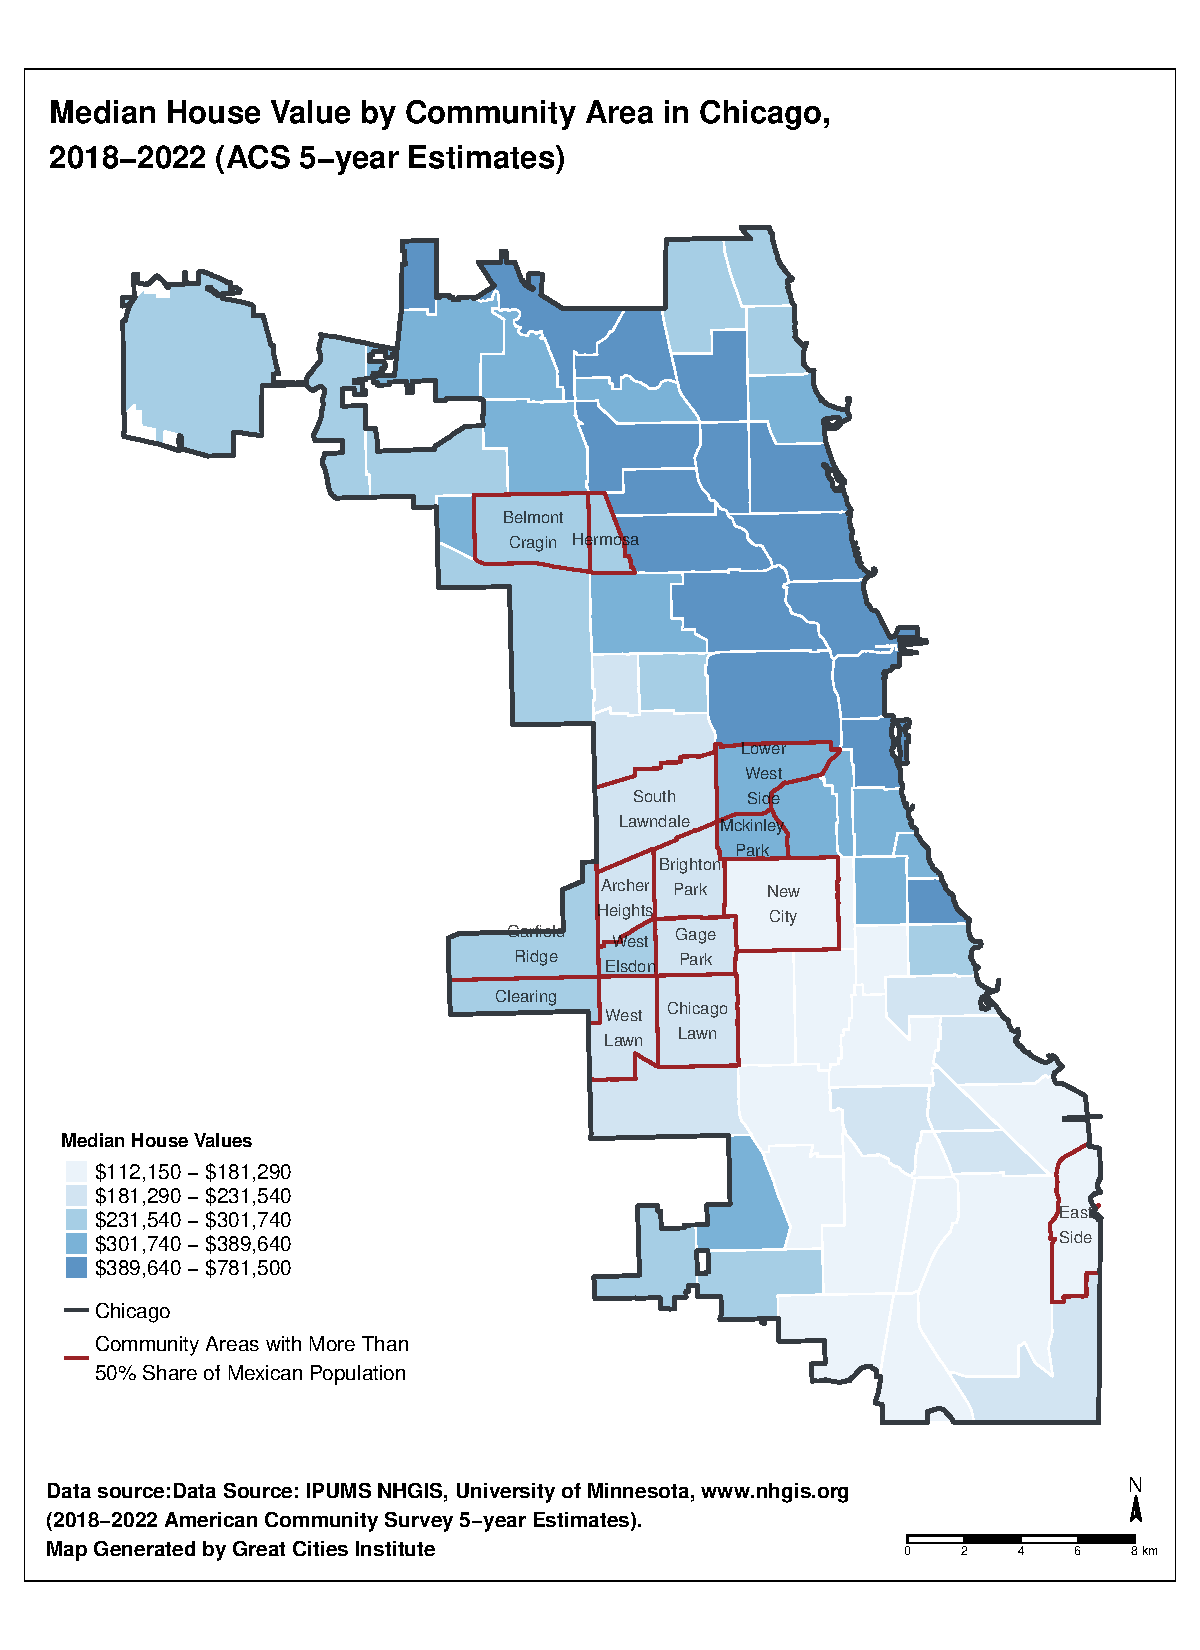
\includegraphics{combined_collar_county_10_files/figure-latex/unnamed-chunk-65-1} \end{center}

\clearpage

\section{Health}\label{health}

\begin{table}[H]
\centering
\begin{threeparttable}
\caption{\label{tab:unnamed-chunk-67}No Health Insurance for Mexicans and Other Racial/Ethnic Groups in Chicago, 2018-2022 (ACS 5-year Estimates)}
\centering
\fontsize{8}{10}\selectfont
\begin{tabular}[t]{>{\raggedright\arraybackslash}p{14.2em}>{\raggedleft\arraybackslash}p{8.6em}>{\raggedleft\arraybackslash}p{8.6em}>{\raggedleft\arraybackslash}p{8.6em}}
\toprule
\multicolumn{1}{>{\centering\arraybackslash}p{14.2em}}{\begingroup\fontsize{8}{10}\selectfont \textbf{Race/Ethnicity}\endgroup} & \multicolumn{1}{>{\centering\arraybackslash}p{8.6em}}{\begingroup\fontsize{8}{10}\selectfont \textbf{Number Without Health Insurance}\endgroup} & \multicolumn{1}{>{\centering\arraybackslash}p{8.6em}}{\begingroup\fontsize{8}{10}\selectfont \textbf{No Insurance Rate}\endgroup} & \multicolumn{1}{>{\centering\arraybackslash}p{8.6em}}{\begingroup\fontsize{8}{10}\selectfont \textbf{Percent Share of the Uninsured Population}\endgroup}\\
\midrule
Mexican & 94,541 & 18.2\% & 40.2\%\\
Other Hispanics or Latinos & 24,171 & 12.5\% & 10.3\%\\
White (non-Hispanic or Latino) & 36,207 & 4.6\% & 15.4\%\\
Black (non-Hispanic or Latino) & 60,337 & 8.8\% & 25.7\%\\
Other (non-Hispanic or Latino) & 19,656 & 8.3\% & 8.4\%\\
\bottomrule
\end{tabular}
\begin{tablenotes}
\small
\item [] \footnotesize{Data Source: IPUMS USA, University of Minnesota, www.ipums.org (2018-2022 American Community Survey 5-year Estimates). Tabulations by Great Cities Institute.}
\end{tablenotes}
\end{threeparttable}
\end{table}

\begin{table}[H]
\centering
\begin{threeparttable}
\caption{\label{tab:unnamed-chunk-69}Number and Percent of Mexico Born and U.S. Born Mexicans Without Job Provided Health Insurance in Chicago, 2018-2022 (ACS 5-year Estimates)}
\centering
\fontsize{8}{10}\selectfont
\begin{tabular}[t]{>{\raggedright\arraybackslash}p{14.2em}>{\raggedleft\arraybackslash}p{7.9em}>{\raggedleft\arraybackslash}p{7.9em}}
\toprule
\multicolumn{1}{>{\centering\arraybackslash}p{14.2em}}{\begingroup\fontsize{8}{10}\selectfont \textbf{Mexican Nativity}\endgroup} & \multicolumn{1}{>{\centering\arraybackslash}p{7.9em}}{\begingroup\fontsize{8}{10}\selectfont \textbf{Number Without Job Provided Health Insurance}\endgroup} & \multicolumn{1}{>{\centering\arraybackslash}p{7.9em}}{\begingroup\fontsize{8}{10}\selectfont \textbf{No Job Provided Health Insurance}\endgroup}\\
\midrule
Mexico Born & 119,608 & 61.8\%\\
U.S. Born & 168,385 & 52.8\%\\
\bottomrule
\end{tabular}
\begin{tablenotes}
\small
\item [] \footnotesize{Data Source: IPUMS NHGIS, University of Minnesota, www.nhgis.org (2018-2022 American Community Survey 5-year Estimates). Tabulations by Great Cities Institute. }
\end{tablenotes}
\end{threeparttable}
\end{table}

\begin{table}[H]
\centering
\begin{threeparttable}
\caption{\label{tab:unnamed-chunk-71}Health Outcomes for Four Communities with the Largest Share of Mexican Population and by Race/Ethnicity in Chicago, 2017-2021, and 2022-2023}
\centering
\fontsize{8}{10}\selectfont
\begin{tabular}[t]{>{\raggedright\arraybackslash}p{14.2em}>{\raggedleft\arraybackslash}p{6.45em}>{\raggedleft\arraybackslash}p{6.45em}>{\raggedleft\arraybackslash}p{6.45em}>{\raggedleft\arraybackslash}p{6.45em}}
\toprule
\multicolumn{1}{>{\centering\arraybackslash}p{14.2em}}{\begingroup\fontsize{8}{10}\selectfont \textbf{Four Communities with the Largest Share of Mexican Population}\endgroup} & \multicolumn{1}{>{\centering\arraybackslash}p{6.45em}}{\begingroup\fontsize{8}{10}\selectfont \textbf{Adult Obesity Rate(2022-2023)}\endgroup} & \multicolumn{1}{>{\centering\arraybackslash}p{6.45em}}{\begingroup\fontsize{8}{10}\selectfont \textbf{Adult Diabetes Rate(2022-2023)}\endgroup} & \multicolumn{1}{>{\centering\arraybackslash}p{6.45em}}{\begingroup\fontsize{8}{10}\selectfont \textbf{Adult Asthma Rate(2022-2023)}\endgroup} & \multicolumn{1}{>{\centering\arraybackslash}p{6.45em}}{\begingroup\fontsize{8}{10}\selectfont \textbf{Low Birthweight Rate(2017-2021)}\endgroup}\\
\midrule
Gage Park & 44.2\% & 18.9\% & 1.9\% & 7.1\%\\
East Side & 52.6\% & 15.2\% & 12.1\% & 6.9\%\\
West Lawn & 38.4\% & 22.2\% & - & 7.1\%\\
South Lawndale & 41.9\% & 25.7\% & 6.0\% & 8.0\%\\
\midrule
\cellcolor{}{\textbf{White (non-Hispanic or Latino) Chicago Mean}} & \cellcolor{}{\textbf{24.5\%}} & \cellcolor{}{\textbf{6.9\%}} & \cellcolor{}{\textbf{9.1\%}} & \cellcolor{}{\textbf{6.2\%}}\\
\cellcolor{}{\textbf{Black (non-Hispanic or Latino) Chicago Mean}} & \cellcolor{}{\textbf{47.6\%}} & \cellcolor{}{\textbf{19.6\%}} & \cellcolor{}{\textbf{14.9\%}} & \cellcolor{}{\textbf{14.6\%}}\\
\cellcolor{}{\textbf{Hispanic or Latino Chicago Mean}} & \cellcolor{}{\textbf{39.9\%}} & \cellcolor{}{\textbf{13.9\%}} & \cellcolor{}{\textbf{9.7\%}} & \cellcolor{}{\textbf{8.0\%}}\\
\bottomrule
\end{tabular}
\begin{tablenotes}
\small
\item [] \footnotesize{Note: Obesity is defined as percent of adults who reported a height and weight that yield a body mass index of 30 or greater.}
\item [] \footnotesize{Diabetes is defined as percent of adults who reported that a doctor, nurse or other health professional has diagnosed them with diabetes.}
\item [] \footnotesize{Asthma is defined as percent of adults who reported that a doctor, nurse or other health professional has diagnosed them with asthma.}
\item [] \footnotesize{Low birthweight is defined as percent of births with a birthweight less than 2500 grams (5.5 pounds).}
\item [] \footnotesize{Data Source:Chicago Health Atlas, Chicago Department of Public Health (2022–2023) and Illinois Department of Public Health (2017-2021). Tabulations by Great Cities Institute}
\end{tablenotes}
\end{threeparttable}
\end{table}

\begin{table}[H]
\centering
\begin{threeparttable}
\caption{\label{tab:unnamed-chunk-73}Mental Health Outcomes for Four Communities with the Largest Share of Mexican Population and by Race/Ethnicity in Chicago, 2022-2023}
\centering
\fontsize{8}{10}\selectfont
\begin{tabular}[t]{>{\raggedright\arraybackslash}p{14.2em}>{\raggedleft\arraybackslash}p{9.2em}>{\raggedleft\arraybackslash}p{9.2em}>{\raggedleft\arraybackslash}p{9.2em}}
\toprule
\multicolumn{1}{>{\centering\arraybackslash}p{14.2em}}{\begingroup\fontsize{8}{10}\selectfont \textbf{Four Communities with the Largest Share of Mexican Population}\endgroup} & \multicolumn{1}{>{\centering\arraybackslash}p{9.2em}}{\begingroup\fontsize{8}{10}\selectfont \textbf{Adult Serious Psych Distress Rate(2022-2023)}\endgroup} & \multicolumn{1}{>{\centering\arraybackslash}p{9.2em}}{\begingroup\fontsize{8}{10}\selectfont \textbf{Adult Unmet Mental Health Need Rate(2022-2023)}\endgroup} & \multicolumn{1}{>{\centering\arraybackslash}p{9.2em}}{\begingroup\fontsize{8}{10}\selectfont \textbf{Adult Loneliness Rate(2022-2023)}\endgroup}\\
\midrule
Gage Park & 13.4\% & 77.4\% & 33.4\%\\
East Side & 10.7\% & 77.1\% & 34.2\%\\
West Lawn & 7.3\% & 78.9\% & 15.6\%\\
South Lawndale & 11.9\% & 78.3\% & 41.5\%\\
\midrule
\cellcolor{}{\textbf{White (non-Hispanic or Latino) Chicago Mean}} & \cellcolor{}{\textbf{7.5\%}} & \cellcolor{}{\textbf{57.2\%}} & \cellcolor{}{\textbf{26.5\%}}\\
\cellcolor{}{\textbf{Black (non-Hispanic or Latino) Chicago Mean}} & \cellcolor{}{\textbf{9.9\%}} & \cellcolor{}{\textbf{81.4\%}} & \cellcolor{}{\textbf{30.2\%}}\\
\cellcolor{}{\textbf{Hispanic or Latino Chicago Mean}} & \cellcolor{}{\textbf{14.9\%}} & \cellcolor{}{\textbf{80.0\%}} & \cellcolor{}{\textbf{29.9\%}}\\
\bottomrule
\end{tabular}
\begin{tablenotes}
\small
\item [] \footnotesize{Note: Serious Psychological Distress is the percent of adults who experienced feelings of nervousness, hopelessness, and depression, in the past 30 days.}
\item [] \footnotesize{Unmet mental health need is the percent of adults with psychological distress who are not receiving treatment or medication.}
\item [] \footnotesize{Loneliness rate is defined as the percent of adults who reported feeling left out or felt alone.}
\item [] \footnotesize{Data Source: Chicago Health Atlas, Chicago Department of Public Health (2022–2023) and Illinois Department of Public Health (2017-2021).Tabulations by Great Cities Institute.}
\end{tablenotes}
\end{threeparttable}
\end{table}

\begin{table}[H]
\centering
\begin{threeparttable}
\caption{\label{tab:unnamed-chunk-75}Chronic Health Indicators for Four Communities with the Largest Share of Mexican Population and by Race/Ethnicity in Chicago, (2017-2021, and 2022-2023)}
\centering
\fontsize{8}{10}\selectfont
\begin{tabular}[t]{>{\raggedright\arraybackslash}p{14.2em}>{\raggedleft\arraybackslash}p{9.2em}>{\raggedleft\arraybackslash}p{9.2em}>{\raggedleft\arraybackslash}p{9.2em}}
\toprule
\multicolumn{1}{>{\centering\arraybackslash}p{14.2em}}{\begingroup\fontsize{8}{10}\selectfont \textbf{Top 4 Community Areas with the Largest Mexican Population Share}\endgroup} & \multicolumn{1}{>{\centering\arraybackslash}p{9.2em}}{\begingroup\fontsize{8}{10}\selectfont \textbf{Adult Cancer Diagnosis Rate per 100,000 (2017-2021)}\endgroup} & \multicolumn{1}{>{\centering\arraybackslash}p{9.2em}}{\begingroup\fontsize{8}{10}\selectfont \textbf{Adult Hypertension Rate (2022-2023)}\endgroup} & \multicolumn{1}{>{\centering\arraybackslash}p{9.2em}}{\begingroup\fontsize{8}{10}\selectfont \textbf{Adult Lung Cancer Diagnosis Rate per 100,000 (2017-2021)}\endgroup}\\
\midrule
Gage Park & 340.0 & 29.5\% & 26.3\\
East Side & 461.8 & 37.2\% & 41.3\\
West Lawn & 416.5 & 30.2\% & 44.7\\
South Lawndale & 342.7 & 25.7\% & 31.4\\
\midrule
\cellcolor{}{\textbf{White (non-Hispanic or Latino) Chicago Mean}} & \cellcolor{}{\textbf{676.2}} & \cellcolor{}{\textbf{29.8\%}} & \cellcolor{}{\textbf{83.4}}\\
\cellcolor{}{\textbf{Black (non-Hispanic or Latino) Chicago Mean}} & \cellcolor{}{\textbf{529.9}} & \cellcolor{}{\textbf{43.9\%}} & \cellcolor{}{\textbf{77.4}}\\
\cellcolor{}{\textbf{Hispanic or Latino Chicago Mean}} & \cellcolor{}{\textbf{253.3}} & \cellcolor{}{\textbf{25.7\%}} & \cellcolor{}{\textbf{13.9}}\\
\bottomrule
\end{tabular}
\begin{tablenotes}
\small
\item [] \footnotesize{Note: Cancer diagnosis is defined as the annual diagnosis rate for all invasive cancers, excluding pre-cancerous conditions.  All ages, risk-adjusted.}
\item [] \footnotesize{Hypertension is the percentage of adults diagnosed with high blood pressure, excluding borderline or pregnancy-related cases.}
\item [] \footnotesize{Lung cancer is defined as lung and bronchus cancer for ages 15 and over, risk-adjusted.}
\item [] \footnotesize{Data Source: Chicago Health Atlas, Chicago Department of Public Health (2022–2023) and Illinois Department of Public Health (2017-2021).Tabulations by Great Cities Institute.}
\end{tablenotes}
\end{threeparttable}
\end{table}

\clearpage

\section{Employment and Business}\label{employment-and-business}

\begin{table}[H]
\centering
\begin{threeparttable}
\caption{\label{tab:unnamed-chunk-76}Labor Force Status for Mexicans and Other Racial/Ethnic Groups in Chicago, 2018-2022 (ACS 5-year Estimates)}
\centering
\fontsize{8}{10}\selectfont
\begin{tabular}[t]{>{\raggedright\arraybackslash}p{14.2em}>{\raggedleft\arraybackslash}p{6.45em}>{\raggedleft\arraybackslash}p{6.45em}>{\raggedleft\arraybackslash}p{6.45em}>{\raggedleft\arraybackslash}p{6.45em}}
\toprule
\multicolumn{1}{>{\centering\arraybackslash}p{14.2em}}{\begingroup\fontsize{8}{10}\selectfont \textbf{Race/Ethnicity}\endgroup} & \multicolumn{1}{>{\centering\arraybackslash}p{6.45em}}{\begingroup\fontsize{8}{10}\selectfont \textbf{In the Labor Force}\endgroup} & \multicolumn{1}{>{\centering\arraybackslash}p{6.45em}}{\begingroup\fontsize{8}{10}\selectfont \textbf{Employed}\endgroup} & \multicolumn{1}{>{\centering\arraybackslash}p{6.45em}}{\begingroup\fontsize{8}{10}\selectfont \textbf{Unemployed}\endgroup} & \multicolumn{1}{>{\centering\arraybackslash}p{6.45em}}{\begingroup\fontsize{8}{10}\selectfont \textbf{Unemployment Rate}\endgroup}\\
\midrule
Mexican & 263,068 & 242,677 & 20,391 & 7.8\%\\
Other Hispanics or Latinos & 102,569 & 95,189 & 7,380 & 7.2\%\\
White (non-Hispanic or Latino) & 504,107 & 482,183 & 21,924 & 4.3\%\\
Black (non-Hispanic or Latino) & 322,796 & 274,277 & 48,519 & 15.0\%\\
Other (non-Hispanic or Latino) & 133,767 & 126,707 & 7,060 & 5.3\%\\
\bottomrule
\end{tabular}
\begin{tablenotes}
\small
\item [] \footnotesize{Data Source: IPUMS USA, University of Minnesota, www.ipums.org (2018-2022 American Community Survey 5-year Estimates). Tabulations by Great Cities Institute.}
\end{tablenotes}
\end{threeparttable}
\end{table}

\begin{center}\includegraphics{combined_collar_county_10_files/figure-latex/unnamed-chunk-77-1} \end{center}

\clearpage

\begin{landscape}

\begingroup\fontsize{7.5}{9.5}\selectfont

\begin{ThreePartTable}
\begin{TableNotes}
\item \footnotesize{Data Source: IPUMS USA, University of Minnesota, www.ipums.org (2018-2022 American Community Survey 5-year Estimates). Tabulations by Great Cities Institute.}
\end{TableNotes}
\begin{longtable}[t]{>{\raggedright\arraybackslash}p{13em}>{\raggedleft\arraybackslash}p{5.2em}>{\raggedleft\arraybackslash}p{5.2em}>{\raggedleft\arraybackslash}p{5.2em}>{\raggedleft\arraybackslash}p{5.2em}>{\raggedleft\arraybackslash}p{5.2em}>{\raggedleft\arraybackslash}p{5.2em}>{\raggedleft\arraybackslash}p{5.2em}>{\raggedleft\arraybackslash}p{5.2em}>{\raggedleft\arraybackslash}p{5.2em}>{\raggedleft\arraybackslash}p{5.2em}}
\caption{\label{tab:unnamed-chunk-78}Employment by Industry and Percent Share of Industry Employment for Mexicans and Other Racial/Ethnic Groups in Chicago, 2018-2022 (ACS 5-year Estimates)}\\
\toprule
\multicolumn{1}{c}{\bgroup\fontsize{7.5}{9.5}\selectfont \textbf{Industry}\egroup{}} & \multicolumn{2}{c}{\bgroup\fontsize{7.5}{9.5}\selectfont \textbf{Mexican}\egroup{}} & \multicolumn{2}{c}{\bgroup\fontsize{7.5}{9.5}\selectfont \textbf{\makecell[c]{Other Hispanics\\or Latinos}}\egroup{}} & \multicolumn{2}{c}{\bgroup\fontsize{7.5}{9.5}\selectfont \textbf{\makecell[c]{White\\(non-Hispanic or Latino)}}\egroup{}} & \multicolumn{2}{c}{\bgroup\fontsize{7.5}{9.5}\selectfont \textbf{\makecell[c]{Black\\(non-Hispanic or Latino)}}\egroup{}} & \multicolumn{2}{c}{\bgroup\fontsize{7.5}{9.5}\selectfont \textbf{\makecell[c]{Other\\(non-Hispanic or Latino)}}\egroup{}} \\
\cmidrule(l{3pt}r{3pt}){1-1} \cmidrule(l{3pt}r{3pt}){2-3} \cmidrule(l{3pt}r{3pt}){4-5} \cmidrule(l{3pt}r{3pt}){6-7} \cmidrule(l{3pt}r{3pt}){8-9} \cmidrule(l{3pt}r{3pt}){10-11}
\multicolumn{1}{>{\centering\arraybackslash}p{13em}}{\begingroup\fontsize{7}{9}\selectfont \endgroup} & \multicolumn{1}{>{\centering\arraybackslash}p{5.2em}}{\begingroup\fontsize{7}{9}\selectfont Number\endgroup} & \multicolumn{1}{>{\centering\arraybackslash}p{5.2em}}{\begingroup\fontsize{7}{9}\selectfont \% Share of Industry Employment\endgroup} & \multicolumn{1}{>{\centering\arraybackslash}p{5.2em}}{\begingroup\fontsize{7}{9}\selectfont Number\endgroup} & \multicolumn{1}{>{\centering\arraybackslash}p{5.2em}}{\begingroup\fontsize{7}{9}\selectfont \% Share of Industry Employment\endgroup} & \multicolumn{1}{>{\centering\arraybackslash}p{5.2em}}{\begingroup\fontsize{7}{9}\selectfont Number\endgroup} & \multicolumn{1}{>{\centering\arraybackslash}p{5.2em}}{\begingroup\fontsize{7}{9}\selectfont \% Share of Industry Employment\endgroup} & \multicolumn{1}{>{\centering\arraybackslash}p{5.2em}}{\begingroup\fontsize{7}{9}\selectfont Number\endgroup} & \multicolumn{1}{>{\centering\arraybackslash}p{5.2em}}{\begingroup\fontsize{7}{9}\selectfont \% Share of Industry Employment\endgroup} & \multicolumn{1}{>{\centering\arraybackslash}p{5.2em}}{\begingroup\fontsize{7}{9}\selectfont Number\endgroup} & \multicolumn{1}{>{\centering\arraybackslash}p{5.2em}}{\begingroup\fontsize{7}{9}\selectfont \% Share of Industry Employment\endgroup}\\
\midrule
Agriculture, Forestry, Fishing, and Hunting, and Mining & 790 & 32.2\% & 279 & 11.4\% & 825 & 33.7\% & 406 & 16.6\% & 151 & 6.2\%\\
Arts, Entertainment, and Recreation, and Accommodation and Food Services & 34,953 & 30.6\% & 10,864 & 9.5\% & 36,015 & 31.5\% & 21,864 & 19.1\% & 10,630 & 9.3\%\\
Construction & 19,912 & 41.8\% & 5,011 & 10.5\% & 16,452 & 34.5\% & 4,676 & 9.8\% & 1,614 & 3.4\%\\
Educational Services, and Health Care and Social Assistance & 38,856 & 13.3\% & 21,313 & 7.3\% & 113,756 & 38.8\% & 80,668 & 27.5\% & 38,409 & 13.1\%\\
Finance and Insurance, and Real Estate, and Rental and Leasing & 12,055 & 11.7\% & 6,208 & 6.0\% & 54,983 & 53.5\% & 18,204 & 17.7\% & 11,227 & 10.9\%\\
\addlinespace
Information & 2,042 & 8.0\% & 910 & 3.5\% & 15,798 & 61.5\% & 3,905 & 15.2\% & 3,042 & 11.8\%\\
Manufacturing & 35,039 & 36.4\% & 9,972 & 10.4\% & 27,629 & 28.7\% & 15,110 & 15.7\% & 8,461 & 8.8\%\\
Military & 115 & 14.9\% & 173 & 22.4\% & 139 & 18.0\% & 234 & 30.3\% & 110 & 14.3\%\\
Other Services, Except Public Administration & 13,696 & 23.0\% & 5,333 & 9.0\% & 21,290 & 35.8\% & 12,343 & 20.8\% & 6,815 & 11.5\%\\
Professional, Scientific, and Management, and Administrative, and Waste Management Services & 29,970 & 13.8\% & 12,926 & 6.0\% & 115,576 & 53.3\% & 33,261 & 15.3\% & 25,098 & 11.6\%\\
\addlinespace
Public Administration & 6,369 & 13.4\% & 3,836 & 8.0\% & 16,659 & 34.9\% & 18,283 & 38.3\% & 2,535 & 5.3\%\\
Retail Trade & 26,380 & 26.1\% & 10,036 & 9.9\% & 29,995 & 29.7\% & 25,341 & 25.1\% & 9,202 & 9.1\%\\
Transportation and Warehousing, and Utilities & 16,549 & 18.6\% & 6,486 & 7.3\% & 22,081 & 24.9\% & 36,420 & 41.0\% & 7,229 & 8.1\%\\
Wholesale Trade & 5,951 & 24.3\% & 1,842 & 7.5\% & 10,985 & 44.8\% & 3,562 & 14.5\% & 2,184 & 8.9\%\\
\bottomrule
\insertTableNotes
\end{longtable}
\end{ThreePartTable}
\endgroup{}

\end{landscape}

\begingroup\fontsize{8}{10}\selectfont

\begin{ThreePartTable}
\begin{TableNotes}
\item \footnotesize{Data Source: IPUMS USA, University of Minnesota, www.ipums.org (2018-2022 American Community Survey 5-year Estimates). Tabulations by Great Cities Institute.}
\end{TableNotes}
\begin{longtable}[t]{>{\raggedright\arraybackslash}p{20em}>{\raggedright\arraybackslash}p{20em}>{\raggedleft\arraybackslash}p{5.5em}>{\raggedleft\arraybackslash}p{5.5em}}
\caption{\label{tab:unnamed-chunk-79}Employment by Industry and Percent Share of Industry Employment for 10 Sub-industries Where Hispanics or Latinos Have the Highest Number of Employees for Mexicans and Other Hispanics or Latinos in Chicago, 2018-2022 (ACS 5-year Estimates)}\\
\toprule
\multicolumn{1}{>{\centering\arraybackslash}p{20em}}{\begingroup\fontsize{8}{10}\selectfont \textbf{Group}\endgroup} & \multicolumn{1}{>{\centering\arraybackslash}p{20em}}{\begingroup\fontsize{8}{10}\selectfont \textbf{Sub-industries}\endgroup} & \multicolumn{1}{>{\centering\arraybackslash}p{5.5em}}{\begingroup\fontsize{8}{10}\selectfont \textbf{Number}\endgroup} & \multicolumn{1}{>{\centering\arraybackslash}p{5.5em}}{\begingroup\fontsize{8}{10}\selectfont \textbf{\% Share of Industry Employment}\endgroup}\\
\midrule
\addlinespace[0.3em]
\multicolumn{4}{l}{\textbf{Mexican}}\\
\hline
Accommodation and Food Services & Restaurants and other food services & 27,844 & 38.1\%\\
Construction & The cleaning of buildings and dwellings is incidental during construction and immediately after construction & 19,912 & 41.8\%\\
Educational Services & Elementary and secondary schools & 9,645 & 15.3\%\\
Health Care and Social Assistance & General medical and surgical hospitals, and specialty (except psychiatric and substance abuse) hospitals & 7,891 & 13.1\%\\
Administrative and support and waste management services & Services to buildings and dwellings (except cleaning during construction and immediately after construction) & 6,590 & 43.1\%\\
Retail Trade & Supermarkets and other grocery (except convenience) stores & 5,869 & 31.5\%\\
Other Services, Except Public Administration & Automotive repair and maintenance & 4,554 & 61.0\%\\
Educational Services & Colleges, universities, and professional schools, including junior colleges & 4,128 & 8.3\%\\
Administrative and support and waste management services & Landscaping services & 3,927 & 70.8\%\\
Manufacturing & Not specified manufacturing industries & 3,636 & 52.3\%\\
\addlinespace[0.3em]
\hline
\multicolumn{4}{l}{\textbf{Other Hispanics or Latinos}}\\
\hline
Accommodation and Food Services & Restaurants and other food services & 7,334 & 10.0\%\\
Educational Services & Elementary and secondary schools & 5,064 & 8.0\%\\
Construction & The cleaning of buildings and dwellings is incidental during construction and immediately after construction & 5,011 & 10.5\%\\
Educational Services & Colleges, universities, and professional schools, including junior colleges & 3,513 & 7.0\%\\
Health Care and Social Assistance & General medical and surgical hospitals, and specialty (except psychiatric and substance abuse) hospitals & 3,383 & 5.6\%\\
Professional, Scientific, and Technical Services & Computer systems design and related services & 2,374 & 7.0\%\\
Administrative and support and waste management services & Services to buildings and dwellings (except cleaning during construction and immediately after construction) & 2,289 & 15.0\%\\
Retail Trade & Supermarkets and other grocery (except convenience) stores & 2,182 & 11.7\%\\
Public Administration & Justice, public order, and safety activities & 1,951 & 8.5\%\\
Health Care and Social Assistance & Child day care services & 1,553 & 11.9\%\\
\bottomrule
\insertTableNotes
\end{longtable}
\end{ThreePartTable}
\endgroup{}

\begin{landscape}

\begingroup\fontsize{8}{10}\selectfont

\begin{ThreePartTable}
\begin{TableNotes}
\item \footnotesize{Data Source: IPUMS USA, University of Minnesota, www.ipums.org (2018-2022 American Community Survey 5-year Estimates). Tabulations by Great Cities Institute.}
\end{TableNotes}
\begin{longtable}[t]{>{\raggedright\arraybackslash}p{13em}>{\raggedleft\arraybackslash}p{5.2em}>{\raggedleft\arraybackslash}p{5.2em}>{\raggedleft\arraybackslash}p{5.2em}>{\raggedleft\arraybackslash}p{5.2em}>{\raggedleft\arraybackslash}p{5.2em}>{\raggedleft\arraybackslash}p{5.2em}>{\raggedleft\arraybackslash}p{5.2em}>{\raggedleft\arraybackslash}p{5.2em}>{\raggedleft\arraybackslash}p{5.2em}>{\raggedleft\arraybackslash}p{5.2em}}
\caption{\label{tab:unnamed-chunk-80}Employment by Occupation and Percent Share of Occupation Employment for Mexicans and Other Racial/Ethnic Groups in Chicago, 2018-2022 (ACS 5-year Estimates)}\\
\toprule
\multicolumn{1}{c}{\bgroup\fontsize{8}{10}\selectfont \textbf{Occupation}\egroup{}} & \multicolumn{2}{c}{\bgroup\fontsize{8}{10}\selectfont \textbf{Mexican}\egroup{}} & \multicolumn{2}{c}{\bgroup\fontsize{8}{10}\selectfont \textbf{\makecell[c]{Other Hispanics\\or Latinos}}\egroup{}} & \multicolumn{2}{c}{\bgroup\fontsize{8}{10}\selectfont \textbf{\makecell[c]{White\\(non-Hispanic or Latino)}}\egroup{}} & \multicolumn{2}{c}{\bgroup\fontsize{8}{10}\selectfont \textbf{\makecell[c]{Black\\(non-Hispanic or Latino)}}\egroup{}} & \multicolumn{2}{c}{\bgroup\fontsize{8}{10}\selectfont \textbf{\makecell[c]{Other\\(non-Hispanic or Latino)}}\egroup{}} \\
\cmidrule(l{3pt}r{3pt}){1-1} \cmidrule(l{3pt}r{3pt}){2-3} \cmidrule(l{3pt}r{3pt}){4-5} \cmidrule(l{3pt}r{3pt}){6-7} \cmidrule(l{3pt}r{3pt}){8-9} \cmidrule(l{3pt}r{3pt}){10-11}
\multicolumn{1}{>{\centering\arraybackslash}p{13em}}{\begingroup\fontsize{7}{9}\selectfont \endgroup} & \multicolumn{1}{>{\centering\arraybackslash}p{5.2em}}{\begingroup\fontsize{7}{9}\selectfont Number\endgroup} & \multicolumn{1}{>{\centering\arraybackslash}p{5.2em}}{\begingroup\fontsize{7}{9}\selectfont \% Share of Occupation Employment\endgroup} & \multicolumn{1}{>{\centering\arraybackslash}p{5.2em}}{\begingroup\fontsize{7}{9}\selectfont Number\endgroup} & \multicolumn{1}{>{\centering\arraybackslash}p{5.2em}}{\begingroup\fontsize{7}{9}\selectfont \% Share of Occupation Employment\endgroup} & \multicolumn{1}{>{\centering\arraybackslash}p{5.2em}}{\begingroup\fontsize{7}{9}\selectfont Number\endgroup} & \multicolumn{1}{>{\centering\arraybackslash}p{5.2em}}{\begingroup\fontsize{7}{9}\selectfont \% Share of Occupation Employment\endgroup} & \multicolumn{1}{>{\centering\arraybackslash}p{5.2em}}{\begingroup\fontsize{7}{9}\selectfont Number\endgroup} & \multicolumn{1}{>{\centering\arraybackslash}p{5.2em}}{\begingroup\fontsize{7}{9}\selectfont \% Share of Occupation Employment\endgroup} & \multicolumn{1}{>{\centering\arraybackslash}p{5.2em}}{\begingroup\fontsize{7}{9}\selectfont Number\endgroup} & \multicolumn{1}{>{\centering\arraybackslash}p{5.2em}}{\begingroup\fontsize{7}{9}\selectfont \% Share of Occupation Employment\endgroup}\\
\midrule
Management, Business, and Financial Occupations & 55,088 & 9.8\% & 32,402 & 5.8\% & 309,194 & 54.8\% & 90,361 & 16.0\% & 76,902 & 13.6\%\\
Natural Resources, Construction, and Maintenance Occupations & 27,822 & 46.8\% & 6,491 & 10.9\% & 15,534 & 26.1\% & 7,415 & 12.5\% & 2,179 & 3.7\%\\
Production, Transportation, and Material Moving Occupations & 55,691 & 36.5\% & 14,999 & 9.8\% & 26,457 & 17.4\% & 45,088 & 29.6\% & 10,129 & 6.7\%\\
Sales and Office Occupations & 46,080 & 20.3\% & 20,492 & 9.0\% & 82,098 & 36.2\% & 59,969 & 26.5\% & 18,128 & 8.0\%\\
Service Occupations & 57,966 & 26.6\% & 20,685 & 9.5\% & 48,802 & 22.4\% & 71,291 & 32.7\% & 19,365 & 8.9\%\\
\bottomrule
\insertTableNotes
\end{longtable}
\end{ThreePartTable}
\endgroup{}

\end{landscape}

\clearpage

\begin{center}\includegraphics{combined_collar_county_10_files/figure-latex/unnamed-chunk-81-1} \end{center}

\clearpage

\begingroup\fontsize{8}{10}\selectfont

\begin{ThreePartTable}
\begin{TableNotes}
\item \footnotesize{Data Source: IPUMS USA, University of Minnesota, www.ipums.org (2018-2022 American Community Survey 5-year Estimates). Tabulations by Great Cities Institute.}
\end{TableNotes}
\begin{longtable}[t]{>{\raggedright\arraybackslash}p{20em}>{\raggedright\arraybackslash}p{20em}>{\raggedleft\arraybackslash}p{5em}>{\raggedleft\arraybackslash}p{6em}}
\caption{\label{tab:unnamed-chunk-82}Employment by Sub-occupation and Percent Share of Occupation Employment for 10 Sub-occupations Where Hispanics or Latinos Have the Highest Number of Employees for Mexicans and Other Hispanics or Latinos in Chicago, 2018-2022 (ACS 5-year Estimates)}\\
\toprule
\multicolumn{1}{>{\centering\arraybackslash}p{20em}}{\begingroup\fontsize{7.5}{9.5}\selectfont \textbf{Occupation Group}\endgroup} & \multicolumn{1}{>{\centering\arraybackslash}p{20em}}{\begingroup\fontsize{7.5}{9.5}\selectfont \textbf{Sub-occupation}\endgroup} & \multicolumn{1}{>{\centering\arraybackslash}p{5em}}{\begingroup\fontsize{7.5}{9.5}\selectfont \textbf{Number}\endgroup} & \multicolumn{1}{>{\centering\arraybackslash}p{6em}}{\begingroup\fontsize{7.5}{9.5}\selectfont \textbf{\% Share of Occupation Employment}\endgroup}\\
\midrule
\addlinespace[0.3em]
\multicolumn{4}{l}{\textbf{Mexican}}\\
\hline
Service Occupations & Janitors and building cleaners & 8,854 & 38.6\%\\
Transportation and Material Moving Occupations & Laborers and freight, stock, and material movers, hand & 8,688 & 41.6\%\\
Service Occupations & Cooks & 7,652 & 44.3\%\\
Sales and Related Occupations & Cashiers & 7,608 & 33.3\%\\
Transportation and Material Moving Occupations & Driver/sales workers and truck drivers & 7,309 & 29.7\%\\
Office and Administrative Support Occupations & Customer service representatives & 5,960 & 21.3\%\\
Construction and Extraction Occupations & Construction laborers & 5,664 & 53.2\%\\
Sales and Related Occupations & Retail salespersons & 4,749 & 24.7\%\\
Service Occupations & Waiters and waitresses & 4,705 & 36.2\%\\
Production Occupations & Miscellaneous production workers, including equipment operators and tenders & 4,375 & 46.8\%\\
\addlinespace[0.3em]
\hline
\multicolumn{4}{l}{\textbf{Other Hispanics or Latinos}}\\
\hline
Service Occupations & Janitors and building cleaners & 2,842 & 12.4\%\\
Office and Administrative Support Occupations & Customer service representatives & 2,546 & 9.1\%\\
Transportation and Material Moving Occupations & Laborers and freight, stock, and material movers, hand & 2,132 & 10.2\%\\
Sales and Related Occupations & Retail salespersons & 2,065 & 10.7\%\\
Transportation and Material Moving Occupations & Driver/sales workers and truck drivers & 2,042 & 8.3\%\\
Management, Business, and Financial Occupations & Other managers & 1,911 & 5.5\%\\
Sales and Related Occupations & First-line supervisors of retail sales workers & 1,896 & 12.4\%\\
Service Occupations & Cooks & 1,882 & 10.9\%\\
Sales and Related Occupations & Cashiers & 1,799 & 7.9\%\\
Construction and Extraction Occupations & Construction laborers & 1,670 & 15.7\%\\
\bottomrule
\insertTableNotes
\end{longtable}
\end{ThreePartTable}
\endgroup{}

\clearpage

\begingroup\fontsize{8}{10}\selectfont

\begin{ThreePartTable}
\begin{TableNotes}
\item \footnotesize{Data Source: IPUMS USA, University of Minnesota, www.ipums.org (2018-2022 American Community Survey 5-year Estimates). Tabulations by Great Cities Institute.}
\end{TableNotes}
\begin{longtable}[t]{>{\raggedright\arraybackslash}p{20em}>{\raggedright\arraybackslash}p{20em}>{\raggedleft\arraybackslash}p{5em}>{\raggedleft\arraybackslash}p{6em}}
\caption{\label{tab:unnamed-chunk-83}Employment by Industry and Percent Share of Occupation Employment for 10 Sub-occupations Where Mexican Males and Females Have the Highest Number of Employees in Chicago, 2018-2022 (ACS 5-year Estimates)}\\
\toprule
\multicolumn{1}{>{\centering\arraybackslash}p{20em}}{\begingroup\fontsize{7.5}{9.5}\selectfont \textbf{Occupation Group}\endgroup} & \multicolumn{1}{>{\centering\arraybackslash}p{20em}}{\begingroup\fontsize{7.5}{9.5}\selectfont \textbf{Sub-occupation}\endgroup} & \multicolumn{1}{>{\centering\arraybackslash}p{5em}}{\begingroup\fontsize{7.5}{9.5}\selectfont \textbf{Number}\endgroup} & \multicolumn{1}{>{\centering\arraybackslash}p{6em}}{\begingroup\fontsize{7.5}{9.5}\selectfont \textbf{\% Share of Occupation Employment}\endgroup}\\
\midrule
\addlinespace[0.3em]
\multicolumn{4}{l}{\textbf{Mexican Males}}\\
\hline
Transportation and Material Moving Occupations & Driver/sales workers and truck drivers & 7,053 & 28.7\%\\
Transportation and Material Moving Occupations & Laborers and freight, stock, and material movers, hand & 6,853 & 32.8\%\\
Service Occupations & Cooks & 5,714 & 33.1\%\\
Construction and Extraction Occupations & Construction laborers & 5,454 & 51.2\%\\
Service Occupations & Janitors and building cleaners & 5,126 & 22.4\%\\
Service Occupations & Landscaping and groundskeeping workers & 3,666 & 71.8\%\\
Installation, Maintenance, and Repair Occupations & Automotive service technicians and mechanics & 3,296 & 56.6\%\\
Construction and Extraction Occupations & Carpenters & 3,254 & 49.1\%\\
Production Occupations & Miscellaneous production workers, including equipment operators and tenders & 2,773 & 29.7\%\\
Construction and Extraction Occupations & Painters and paperhangers & 2,455 & 59.8\%\\
\addlinespace[0.3em]
\hline
\multicolumn{4}{l}{\textbf{Mexican Females}}\\
\hline
Sales and Related Occupations & Cashiers & 5,771 & 25.3\%\\
Service Occupations & Janitors and building cleaners & 3,728 & 16.3\%\\
Office and Administrative Support Occupations & Customer service representatives & 3,588 & 12.8\%\\
Service Occupations & Waiters and waitresses & 2,894 & 22.3\%\\
Sales and Related Occupations & Retail salespersons & 2,858 & 14.8\%\\
Service Occupations & Maids and housekeeping cleaners & 2,509 & 25.4\%\\
Service Occupations & Childcare workers & 2,389 & 21.4\%\\
Office and Administrative Support Occupations & Secretaries and administrative assistants, except legal, medical, and executive & 2,028 & 16.7\%\\
Education, Legal, Community Service, Arts, and Media Occupations & Elementary and middle school teachers & 1,954 & 9.3\%\\
Service Occupations & Cooks & 1,938 & 11.2\%\\
\bottomrule
\insertTableNotes
\end{longtable}
\end{ThreePartTable}
\endgroup{}

\clearpage

\begin{table}[H]
\centering
\begin{threeparttable}
\caption{\label{tab:unnamed-chunk-84}Union Membership and Coverage for Mexicans and Other Racial/Ethnic Groups in the U.S., 2022}
\centering
\fontsize{8}{10}\selectfont
\begin{tabular}[t]{>{\raggedright\arraybackslash}p{14.2em}>{\raggedleft\arraybackslash}p{5.16em}>{\raggedleft\arraybackslash}p{5.16em}>{\raggedleft\arraybackslash}p{5.16em}>{\raggedleft\arraybackslash}p{5.16em}r}
\toprule
\multicolumn{1}{l}{\bgroup\fontsize{8}{10}\selectfont \textbf{Race/Ethnicity}\egroup{}} & \multicolumn{1}{c}{\bgroup\fontsize{8}{10}\selectfont \textbf{\makecell[c]{Total\\Employed}}\egroup{}} & \multicolumn{2}{c}{\bgroup\fontsize{8}{10}\selectfont \textbf{\makecell[c]{Member of\\Labor Union}}\egroup{}} & \multicolumn{2}{c}{\bgroup\fontsize{8}{10}\selectfont \textbf{\makecell[c]{Covered by\\Union but Not\\a Member}}\egroup{}} \\
\cmidrule(l{3pt}r{3pt}){1-1} \cmidrule(l{3pt}r{3pt}){2-2} \cmidrule(l{3pt}r{3pt}){3-4} \cmidrule(l{3pt}r{3pt}){5-6}
\multicolumn{1}{>{\centering\arraybackslash}p{14.2em}}{\begingroup\fontsize{8}{10}\selectfont \textbf{}\endgroup} & \multicolumn{1}{>{\centering\arraybackslash}p{5.16em}}{\begingroup\fontsize{8}{10}\selectfont \textbf{}\endgroup} & \multicolumn{1}{>{\centering\arraybackslash}p{5.16em}}{\begingroup\fontsize{8}{10}\selectfont \textbf{Number}\endgroup} & \multicolumn{1}{>{\centering\arraybackslash}p{5.16em}}{\begingroup\fontsize{8}{10}\selectfont \textbf{Percent}\endgroup} & \multicolumn{1}{>{\centering\arraybackslash}p{5.16em}}{\begingroup\fontsize{8}{10}\selectfont \textbf{Number}\endgroup} & \multicolumn{1}{c}{\begingroup\fontsize{8}{10}\selectfont \textbf{Percent}\endgroup}\\
\midrule
Mexican & 18,101,402 & 1,405,940 & 7.8\% & 66,294 & 0.4\%\\
Other Hispanics or Latinos & 11,031,515 & 1,001,838 & 9.1\% & 118,350 & 1.1\%\\
White (non-Hispanic or Latino) & 96,265,453 & 9,171,730 & 9.5\% & 1,049,954 & 1.1\%\\
Black (non-Hispanic or Latino) & 18,553,017 & 1,727,357 & 9.3\% & 242,419 & 1.3\%\\
Other (non-Hispanic or Latino) & 14,154,300 & 1,024,372 & 7.2\% & 207,312 & 1.5\%\\
\bottomrule
\end{tabular}
\begin{tablenotes}
\small
\item [] \footnotesize{Data Source: IPUMS CPS, University of Minnesota, www.ipums.org. (2022 Current Population Survey). Tabulations by Great Cities Institute.}
\end{tablenotes}
\end{threeparttable}
\end{table}

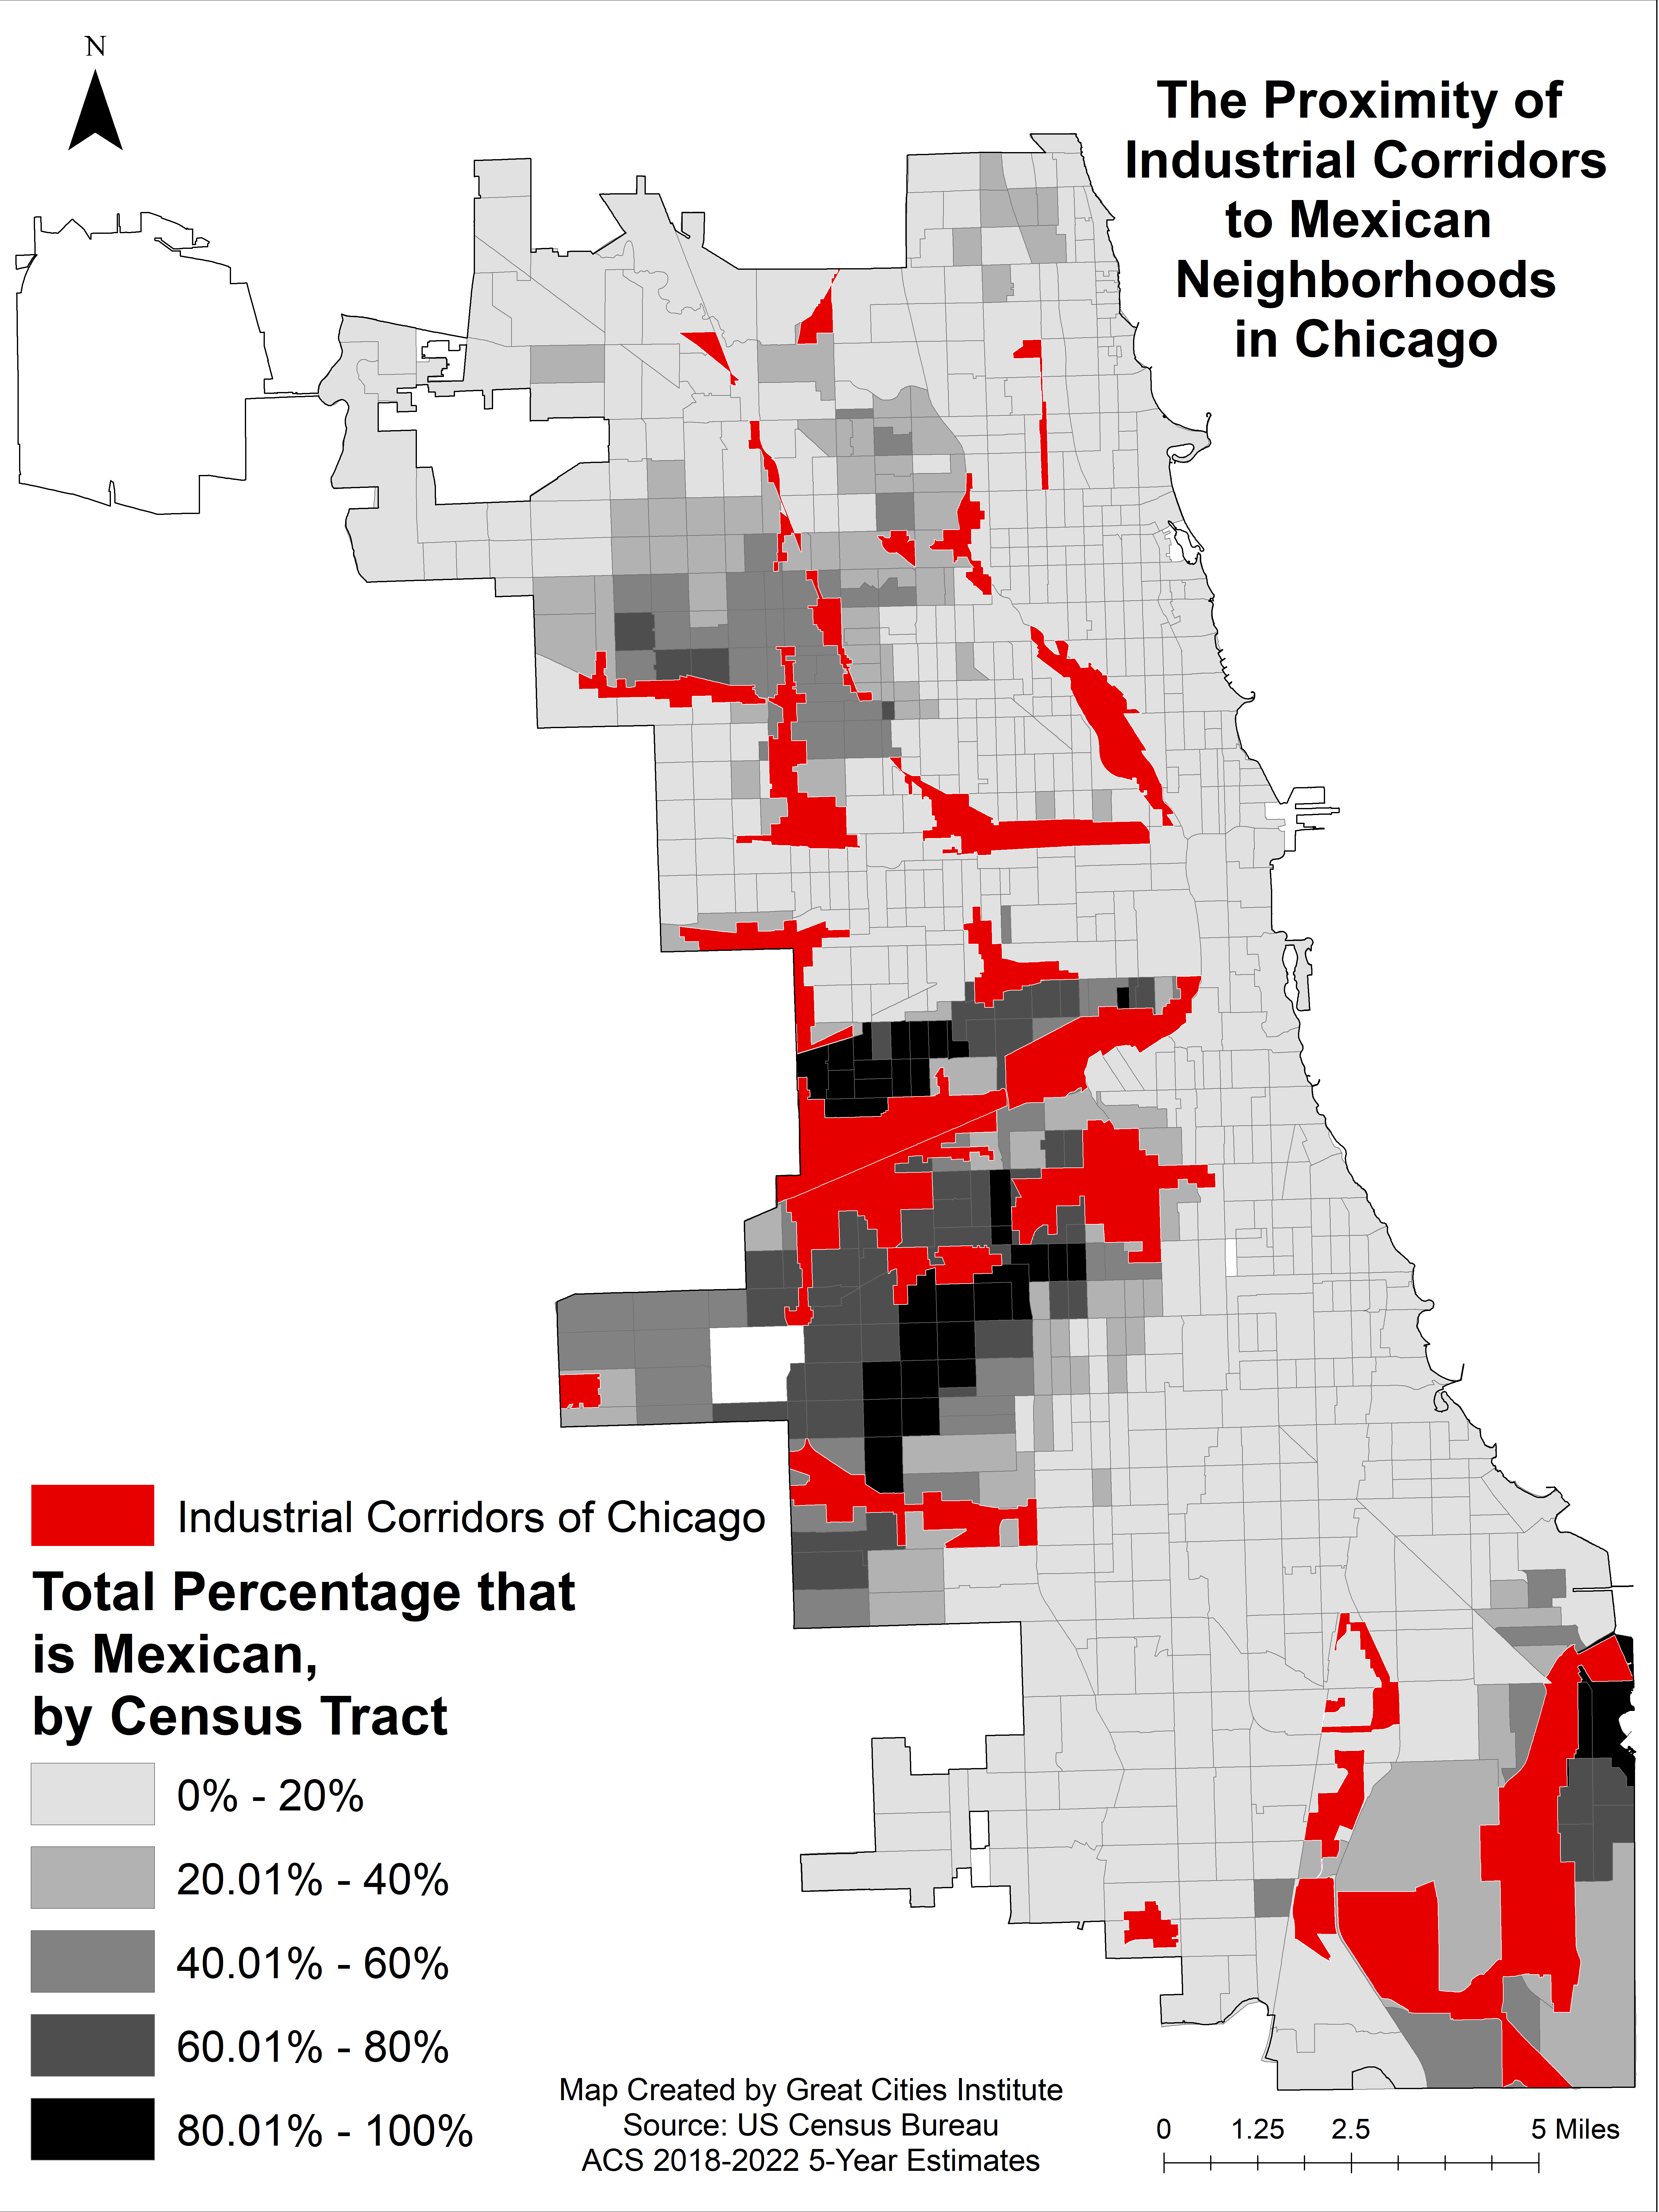
\includegraphics[width=75in]{Data Tables/MexicansChicago_IndustrialCorridors}

\clearpage

\begin{table}[H]
\centering
\caption{\label{tab:unnamed-chunk-86}Primary Means of Transportation to Work for Mexicans and Other Racial/Ethnic Groups in Chicago, 2018-2022 (ACS 5-year Estimates)}
\centering
\fontsize{8}{10}\selectfont
\begin{threeparttable}
\begin{tabular}[t]{>{\raggedright\arraybackslash}p{12em}>{\raggedleft\arraybackslash}p{5.5em}>{\raggedleft\arraybackslash}p{5.5em}>{\raggedleft\arraybackslash}p{5.5em}>{\raggedleft\arraybackslash}p{5.5em}>{\raggedleft\arraybackslash}p{5.5em}>{\raggedleft\arraybackslash}p{5.5em}}
\toprule
\multicolumn{1}{c}{\bgroup\fontsize{8}{10}\selectfont \textbf{\makecell[c]{Means of\\Transportation}}\egroup{}} & \multicolumn{2}{c}{\bgroup\fontsize{8}{10}\selectfont \textbf{Mexican}\egroup{}} & \multicolumn{2}{c}{\bgroup\fontsize{8}{10}\selectfont \textbf{\makecell[c]{Other Hispanics\\or Latinos}}\egroup{}} & \multicolumn{2}{c}{\bgroup\fontsize{8}{10}\selectfont \textbf{\makecell[c]{Non-Hispanic\\or Latino}}\egroup{}} \\
\cmidrule(l{3pt}r{3pt}){1-1} \cmidrule(l{3pt}r{3pt}){2-3} \cmidrule(l{3pt}r{3pt}){4-5} \cmidrule(l{3pt}r{3pt}){6-7}
\multicolumn{1}{>{\centering\arraybackslash}p{12em}}{} & \multicolumn{1}{>{\centering\arraybackslash}p{5.5em}}{Number} & \multicolumn{1}{>{\centering\arraybackslash}p{5.5em}}{Percent} & \multicolumn{1}{>{\centering\arraybackslash}p{5.5em}}{Number} & \multicolumn{1}{>{\centering\arraybackslash}p{5.5em}}{Percent} & \multicolumn{1}{>{\centering\arraybackslash}p{5.5em}}{Number} & \multicolumn{1}{>{\centering\arraybackslash}p{5.5em}}{Percent}\\
\midrule
Auto, truck, or van & 167,218 & 68.9\% & 57,961 & 60.9\% & 424,893 & 48.1\%\\
Bicycle & 1,954 & 0.8\% & 696 & 0.7\% & 12,418 & 1.4\%\\
Bus & 21,894 & 9.0\% & 8,714 & 9.2\% & 90,905 & 10.3\%\\
Light rail, streetcar, or trolley (Carro público in PR) & 252 & 0.1\% & 192 & 0.2\% & 1,353 & 0.1\%\\
Long-distance train or commuter train & 1,475 & 0.6\% & 896 & 0.9\% & 12,148 & 1.4\%\\
Motorcycle & 58 & 0.0\% & 96 & 0.1\% & 362 & 0.0\%\\
Other & 2,820 & 1.2\% & 1,323 & 1.4\% & 10,580 & 1.2\%\\
Subway or elevated & 14,417 & 5.9\% & 6,344 & 6.7\% & 90,438 & 10.2\%\\
Taxicab & 1,477 & 0.6\% & 645 & 0.7\% & 6,624 & 0.8\%\\
Walked only & 8,195 & 3.4\% & 4,101 & 4.3\% & 51,523 & 5.8\%\\
Worked at home & 16,508 & 6.8\% & 11,990 & 12.6\% & 163,431 & 18.5\%\\
Ferryboat & - & - & - & - & 74 & 0.0\%\\
\bottomrule
\end{tabular}
\begin{tablenotes}
\item \footnotesize{Data Source: IPUMS USA, University of Minnesota, www.ipums.org (2018-2022 American Community Survey 5-year Estimates). Tabulations by Great Cities Institute.}
\end{tablenotes}
\end{threeparttable}
\end{table}

\begin{table}[H]
\centering
\caption{\label{tab:unnamed-chunk-87}Illinois and Chicago Metro Area Latino GDP, 2018}
\centering
\fontsize{8}{10}\selectfont
\begin{threeparttable}
\begin{tabular}[t]{>{\raggedright\arraybackslash}p{20em}>{\raggedleft\arraybackslash}p{10em}}
\toprule
\multicolumn{1}{>{\centering\arraybackslash}p{20em}}{\begingroup\fontsize{8}{10}\selectfont \textbf{}\endgroup} & \multicolumn{1}{>{\centering\arraybackslash}p{10em}}{\begingroup\fontsize{8}{10}\selectfont \textbf{Latino GDP (billions of dollars)}\endgroup}\\
\midrule
Illinois Latino GDP (5th highest state) & 100.1\\
Chicago Metro Area (IL, IN, WI) Latino GDP (5th highest metro area) & 97.5\\
\bottomrule
\end{tabular}
\begin{tablenotes}
\item \footnotesize{Data Source: 2023 U.S. Latino GDP Report, www.LatinoGDP.us (CLU-CERF, Bank of America State and Metro Latino GDP Reports).}
\end{tablenotes}
\end{threeparttable}
\end{table}

\begin{table}[H]
\centering
\caption{\label{tab:unnamed-chunk-88}2021 Latino GDP with 10 Largest Countries}
\centering
\fontsize{8}{10}\selectfont
\begin{threeparttable}
\begin{tabular}[t]{>{\raggedright\arraybackslash}p{20em}>{\raggedleft\arraybackslash}p{10em}}
\toprule
\multicolumn{1}{>{\centering\arraybackslash}p{20em}}{\begingroup\fontsize{8}{10}\selectfont \textbf{Country}\endgroup} & \multicolumn{1}{>{\centering\arraybackslash}p{10em}}{\begingroup\fontsize{8}{10}\selectfont \textbf{GDP (billions of dollars)}\endgroup}\\
\midrule
United States & 23,315.1\\
China & 17,759.3\\
Japan & 5,005.5\\
Germany & 4,262.8\\
\cellcolor{}{\textbf{U.S. Latinos}} & \cellcolor{}{\textbf{3,159.7}}\\
India & 3,150.3\\
United Kingdom & 3,123.2\\
France & 2,957.4\\
Italy & 2,115.8\\
Canada & 2,001.5\\
Russia & 1,836.6\\
\bottomrule
\end{tabular}
\begin{tablenotes}
\item \footnotesize{Data Source: 2023 U.S. Latino GDP Report, www.LatinoGDP.us (International Monetary Fund and Organization for Economic Cooperation and Development).}
\end{tablenotes}
\end{threeparttable}
\end{table}

\begin{table}[H]
\centering
\begin{threeparttable}
\caption{\label{tab:unnamed-chunk-89}Median Household Net Worth by Detailed Hispanic Origin, 2020}
\centering
\fontsize{8}{10}\selectfont
\begin{tabular}[t]{>{\raggedright\arraybackslash}p{19em}>{\raggedleft\arraybackslash}p{7em}r}
\toprule
\multicolumn{1}{>{\centering\arraybackslash}p{19em}}{\begingroup\fontsize{8}{10}\selectfont \textbf{Hispanic Origin Group}\endgroup} & \multicolumn{1}{>{\centering\arraybackslash}p{7em}}{\begingroup\fontsize{8}{10}\selectfont \textbf{Median Household Net Worth}\endgroup} & \multicolumn{1}{c}{\begingroup\fontsize{8}{10}\selectfont \textbf{Standard Error}\endgroup}\\
\midrule
Mexican & \$52,440 & \$3,640\\
\hspace{.7em}\em{Native-born Mexican} & \$52,650 & \$3,088\\
\hspace{.7em}\em{Foreign-born Mexican} & \$47,530 & \$5,403\\
Puerto Rican & \$35,770 & \$20,280\\
Cuban & \$92,700 & \$31,780\\
Salvadoran & \$30,600 & \$7,468\\
Dominican & \$9,430 & \$7,428\\
Colombian & \$141,200 & \$72,690\\
Other Hispanic & \$58,490 & \$14,130\\
Not Hispanic & \$195,600 & \$5,202\\
Hispanic & \$52,190 & \$3,260\\
\bottomrule
\end{tabular}
\begin{tablenotes}
\small
\item [] \footnotesize{Note: Use caution with estimates having coefficients of variation (defined as the standard error divided by the estimate) larger than 0.3 as they may suffer from data quality issues.}
\item [] \footnotesize{Source: U.S. Census Bureau, 2021 Survey of Income and Program Participation, public-use data.}
\item [] \footnotesize{Reproduced from a table by: Zachary Scherer and Yerís H. Mayol-García, statisticians in the Census Bureau’s Social, Economic, and Housing Statistics Division.}
\end{tablenotes}
\end{threeparttable}
\end{table}

\begin{table}[H]
\centering
\begin{threeparttable}
\caption{\label{tab:unnamed-chunk-90}Share of Business Ownership (2021) and Population by Race/Ethnicity (2018-2022 ACS 5-year Estimates) in Chicago−Naperville−Elgin, IL−IN−WI Metro Area}
\centering
\fontsize{8}{10}\selectfont
\begin{tabular}[t]{>{\raggedright\arraybackslash}p{19em}>{\raggedleft\arraybackslash}p{7em}rr}
\toprule
\multicolumn{1}{>{\centering\arraybackslash}p{19em}}{\begingroup\fontsize{8}{10}\selectfont \textbf{Ownership}\endgroup} & \multicolumn{1}{>{\centering\arraybackslash}p{7em}}{\begingroup\fontsize{8}{10}\selectfont \textbf{Without Employees}\endgroup} & \multicolumn{1}{c}{\begingroup\fontsize{8}{10}\selectfont \textbf{With Employees}\endgroup} & \multicolumn{1}{c}{\begingroup\fontsize{8}{10}\selectfont \textbf{Total Businesses}\endgroup}\\
\midrule
Hispanic & 124,000 & 15,499 & 139,499\\
Not Hispanic & 708,000 & 173,587 & 881,587\\
Owned equally by both groups & 1,200 & 1,216 & 2,416\\
\midrule
%\\
American Indian and Alaska Native (non-Hispanic) & 3,000 & 441 & 3,441\\
Asian (non-Hispanic) & 80,000 & 20,290 & 100,290\\
Black or African American (non-Hispanic) & 146,000 & 5,541 & 151,541\\
Native Hawaiian and Other Pacific Islander (non-Hispanic) & 700 & 71 & 771\\
White (non-Hispanic) & 488,000 & 147,353 & 635,353\\
\bottomrule
\end{tabular}
\begin{tablenotes}
\small
\item [] \footnotesize{Note: Counts include only businesses classifiable by owner demographic group}
\item [] \footnotesize{Data Sources: Annual Business Survey, 2021 (Census); Nonemployer Statistics by Demographics, 2021 (Census)
}
\end{tablenotes}
\end{threeparttable}
\end{table}

\begin{center}\includegraphics{combined_collar_county_10_files/figure-latex/unnamed-chunk-91-1} \end{center}

\begin{landscape}

\begin{table}[H]
\centering
\begin{threeparttable}
\caption{\label{tab:unnamed-chunk-92}Race/Ethnicity Status of C-Suite Executives for Top 50 Companies in Chicago, 2012-2022}
\centering
\fontsize{8}{10}\selectfont
\begin{tabular}[t]{>{\raggedright\arraybackslash}p{10em}>{}r>{}r>{}r>{}r>{}r>{}r>{}r>{}r>{}r>{}r>{}r>{}r>{}r}
\toprule
\multicolumn{1}{l}{\bgroup\fontsize{8}{10}\selectfont \textbf{Race/Ethnicity}\egroup{}} & \multicolumn{2}{c}{\bgroup\fontsize{8}{10}\selectfont \textbf{2012}\egroup{}} & \multicolumn{2}{c}{\bgroup\fontsize{8}{10}\selectfont \textbf{2014}\egroup{}} & \multicolumn{2}{c}{\bgroup\fontsize{8}{10}\selectfont \textbf{2016}\egroup{}} & \multicolumn{2}{c}{\bgroup\fontsize{8}{10}\selectfont \textbf{2018}\egroup{}} & \multicolumn{2}{c}{\bgroup\fontsize{8}{10}\selectfont \textbf{2020}\egroup{}} & \multicolumn{2}{c}{\bgroup\fontsize{8}{10}\selectfont \textbf{2022}\egroup{}} & \multicolumn{1}{c}{\bgroup\fontsize{8}{10}\selectfont \textbf{2012-2022}\egroup{}} \\
\cmidrule(l{3pt}r{3pt}){1-1} \cmidrule(l{3pt}r{3pt}){2-3} \cmidrule(l{3pt}r{3pt}){4-5} \cmidrule(l{3pt}r{3pt}){6-7} \cmidrule(l{3pt}r{3pt}){8-9} \cmidrule(l{3pt}r{3pt}){10-11} \cmidrule(l{3pt}r{3pt}){12-13} \cmidrule(l{3pt}r{3pt}){14-14}
\multicolumn{1}{>{\centering\arraybackslash}p{7em}}{\begingroup\fontsize{8}{10}\selectfont \endgroup} & \multicolumn{1}{>{\centering\arraybackslash}p{2.3em}}{\begingroup\fontsize{8}{10}\selectfont Number\endgroup} & \multicolumn{1}{>{\centering\arraybackslash}p{2.3em}}{\begingroup\fontsize{8}{10}\selectfont Percent\endgroup} & \multicolumn{1}{>{\centering\arraybackslash}p{2.3em}}{\begingroup\fontsize{8}{10}\selectfont Number\endgroup} & \multicolumn{1}{>{\centering\arraybackslash}p{2.3em}}{\begingroup\fontsize{8}{10}\selectfont Percent\endgroup} & \multicolumn{1}{>{\centering\arraybackslash}p{2.3em}}{\begingroup\fontsize{8}{10}\selectfont Number\endgroup} & \multicolumn{1}{>{\centering\arraybackslash}p{2.3em}}{\begingroup\fontsize{8}{10}\selectfont Percent\endgroup} & \multicolumn{1}{>{\centering\arraybackslash}p{2.3em}}{\begingroup\fontsize{8}{10}\selectfont Number\endgroup} & \multicolumn{1}{>{\centering\arraybackslash}p{2.3em}}{\begingroup\fontsize{8}{10}\selectfont Percent\endgroup} & \multicolumn{1}{>{\centering\arraybackslash}p{2.3em}}{\begingroup\fontsize{8}{10}\selectfont Number\endgroup} & \multicolumn{1}{>{\centering\arraybackslash}p{2.3em}}{\begingroup\fontsize{8}{10}\selectfont Percent\endgroup} & \multicolumn{1}{>{\centering\arraybackslash}p{2.3em}}{\begingroup\fontsize{8}{10}\selectfont Number\endgroup} & \multicolumn{1}{>{\centering\arraybackslash}p{2.3em}}{\begingroup\fontsize{8}{10}\selectfont Percent\endgroup} & \multicolumn{1}{>{\centering\arraybackslash}p{3.5em}}{\begingroup\fontsize{8}{10}\selectfont Percentage Point Difference\endgroup}\\
\midrule
Caucasian & 166 & 80.2\% & 163 & 81.5\% & 174 & 85.3\% & 184 & 85.2\% & 210 & 82.7\% & 221 & 79.5\% & -0.7\%\\
African-American & 4 & 1.9\% & 8 & 4.0\% & 7 & 3.4\% & 11 & 5.1\% & 16 & 6.3\% & 23 & 8.3\% & 6.3\%\\
Hispanic & 2 & 1.0\% & 3 & 1.5\% & 4 & 2.0\% & 6 & 2.8\% & 12 & 4.7\% & 7 & 2.5\% & 1.6\%\\
Asian & 8 & 3.9\% & 6 & 3.0\% & 6 & 2.9\% & 5 & 2.3\% & 15 & 5.9\% & 27 & 9.7\% & 5.8\%\\
Unable to Verify Ethnicity & 27 & 13.0\% & 20 & 10.0\% & 13 & 6.4\% & 10 & 4.6\% & 1 & 0.4\% & 0 & 0.0\% & -13.0\%\\
Total & 207 & 100.0\% & 200 & 100.0\% & 204 & 100.0\% & 216 & 100.0\% & 254 & 100.0\% & 278 & 100.0\% & 0.0\%\\
\bottomrule
\end{tabular}
\begin{tablenotes}
\small
\item [] \footnotesize{Data Source: Chicago United Inside Inclusion. Data compiled by Great Cities Institute.}
\end{tablenotes}
\end{threeparttable}
\end{table}

\end{landscape}

\begin{landscape}

\begin{table}[H]
\centering
\begin{threeparttable}
\caption{\label{tab:unnamed-chunk-93}Race/Ethnicity of Boards of Directors for Top 50 Companies in Chicago, 2012-2022}
\centering
\fontsize{8}{10}\selectfont
\begin{tabular}[t]{>{\raggedright\arraybackslash}p{10em}>{}r>{}r>{}r>{}r>{}r>{}r>{}r>{}r>{}r>{}r>{}r>{}r>{\raggedleft\arraybackslash}p{3.5em}}
\toprule
\multicolumn{1}{l}{\bgroup\fontsize{8}{10}\selectfont \textbf{Race/Ethnicity}\egroup{}} & \multicolumn{2}{c}{\bgroup\fontsize{8}{10}\selectfont \textbf{2012}\egroup{}} & \multicolumn{2}{c}{\bgroup\fontsize{8}{10}\selectfont \textbf{2014}\egroup{}} & \multicolumn{2}{c}{\bgroup\fontsize{8}{10}\selectfont \textbf{2016}\egroup{}} & \multicolumn{2}{c}{\bgroup\fontsize{8}{10}\selectfont \textbf{2018}\egroup{}} & \multicolumn{2}{c}{\bgroup\fontsize{8}{10}\selectfont \textbf{2020}\egroup{}} & \multicolumn{2}{c}{\bgroup\fontsize{8}{10}\selectfont \textbf{2022}\egroup{}} & \multicolumn{1}{c}{\bgroup\fontsize{8}{10}\selectfont \textbf{2012-2020}\egroup{}} \\
\cmidrule(l{3pt}r{3pt}){1-1} \cmidrule(l{3pt}r{3pt}){2-3} \cmidrule(l{3pt}r{3pt}){4-5} \cmidrule(l{3pt}r{3pt}){6-7} \cmidrule(l{3pt}r{3pt}){8-9} \cmidrule(l{3pt}r{3pt}){10-11} \cmidrule(l{3pt}r{3pt}){12-13} \cmidrule(l{3pt}r{3pt}){14-14}
\multicolumn{1}{c}{\begingroup\fontsize{8}{10}\selectfont \endgroup} & \multicolumn{1}{c}{\begingroup\fontsize{8}{10}\selectfont Number\endgroup} & \multicolumn{1}{c}{\begingroup\fontsize{8}{10}\selectfont Percent\endgroup} & \multicolumn{1}{c}{\begingroup\fontsize{8}{10}\selectfont Number\endgroup} & \multicolumn{1}{c}{\begingroup\fontsize{8}{10}\selectfont Percent\endgroup} & \multicolumn{1}{c}{\begingroup\fontsize{8}{10}\selectfont Number\endgroup} & \multicolumn{1}{c}{\begingroup\fontsize{8}{10}\selectfont Percent\endgroup} & \multicolumn{1}{c}{\begingroup\fontsize{8}{10}\selectfont Number\endgroup} & \multicolumn{1}{c}{\begingroup\fontsize{8}{10}\selectfont Percent\endgroup} & \multicolumn{1}{c}{\begingroup\fontsize{8}{10}\selectfont Number\endgroup} & \multicolumn{1}{c}{\begingroup\fontsize{8}{10}\selectfont Percent\endgroup} & \multicolumn{1}{c}{\begingroup\fontsize{8}{10}\selectfont Number\endgroup} & \multicolumn{1}{c}{\begingroup\fontsize{8}{10}\selectfont Percent\endgroup} & \multicolumn{1}{c}{\begingroup\fontsize{8}{10}\selectfont Percentage Point Difference\endgroup}\\
\midrule
Caucasian & 540 & 84.2\% & 466 & 84.6\% & 463 & 83.1\% & 461 & 83.1\% & 461 & 83.4\% & 375 & 76.7\% & -7.6\%\\
African-American & 41 & 6.4\% & 34 & 6.2\% & 44 & 7.9\% & 42 & 7.6\% & 50 & 9.0\% & 67 & 13.7\% & 7.3\%\\
Hispanic & 19 & 3.0\% & 19 & 3.4\% & 19 & 3.4\% & 22 & 4.0\% & 23 & 4.2\% & 20 & 4.1\% & 1.1\%\\
Asian & 15 & 2.3\% & 16 & 2.9\% & 14 & 2.5\% & 14 & 2.5\% & 16 & 2.9\% & 23 & 4.7\% & 2.4\%\\
Unable to Verify Ethnicity & 26 & 4.1\% & 16 & 2.9\% & 17 & 3.1\% & 16 & 2.9\% & 3 & 0.5\% & 4 & 0.8\% & -3.2\%\\
Total & 641 & 100.0\% & 551 & 100.0\% & 557 & 100.0\% & 555 & 100.0\% & 553 & 100.0\% & 489 & 100.0\% & 0.0\%\\
\bottomrule
\end{tabular}
\begin{tablenotes}
\small
\item [] \footnotesize{
Data Source: Chicago United Inside Inclusion. Data compiled by Great Cities Institute.}
\end{tablenotes}
\end{threeparttable}
\end{table}

\end{landscape}

\clearpage

\section{Citizenship and Civic
Participation}\label{citizenship-and-civic-participation}

\begin{table}[H]
\centering
\begin{threeparttable}
\caption{\label{tab:unnamed-chunk-95}U.S. Citizenship for Mexicans and Other Racial/Ethnic Groups in Chicago, 2000 (Decennial Census), 2008-2012, and 2018-2022 (ACS 5-year Estimates)}
\centering
\fontsize{8}{10}\selectfont
\begin{tabular}[t]{>{\raggedright\arraybackslash}p{14.2em}>{\raggedleft\arraybackslash}p{6.45em}>{\raggedleft\arraybackslash}p{6.45em}>{\raggedleft\arraybackslash}p{6.45em}>{\raggedleft\arraybackslash}p{6.45em}}
\toprule
\multicolumn{1}{l}{\bgroup\fontsize{8}{10}\selectfont \textbf{Race/Ethnicity}\egroup{}} & \multicolumn{4}{c}{\bgroup\fontsize{8}{10}\selectfont \textbf{Citizen Rate}\egroup{}} \\
\cmidrule(l{3pt}r{3pt}){1-1} \cmidrule(l{3pt}r{3pt}){2-5}
\multicolumn{1}{>{\centering\arraybackslash}p{14.2em}}{\begingroup\fontsize{8}{10}\selectfont \endgroup} & \multicolumn{1}{>{\centering\arraybackslash}p{6.45em}}{\begingroup\fontsize{8}{10}\selectfont 2000\endgroup} & \multicolumn{1}{>{\centering\arraybackslash}p{6.45em}}{\begingroup\fontsize{8}{10}\selectfont 2008-2012\endgroup} & \multicolumn{1}{>{\centering\arraybackslash}p{6.45em}}{\begingroup\fontsize{8}{10}\selectfont 2018-2022\endgroup} & \multicolumn{1}{>{\centering\arraybackslash}p{6.45em}}{\begingroup\fontsize{8}{10}\selectfont Change from 2000 to 2018-2022\endgroup}\\
\midrule
Mexican & 60.7\% & 67.4\% & 77.5\% & 16.8\%\\
Other Hispanics or Latinos & 81.7\% & 84.1\% & 85.5\% & 3.8\%\\
White (non-Hispanic or Latino) & 90.1\% & 93.2\% & 95.1\% & 5.0\%\\
Black (non-Hispanic or Latino) & 98.9\% & 98.3\% & 98.2\% & -0.7\%\\
Other (non-Hispanic or Latino) & 67.1\% & 72.2\% & 76.2\% & 9.1\%\\
\bottomrule
\end{tabular}
\begin{tablenotes}
\small
\item [] \footnotesize{Data Source: IPUMS USA, University of Minnesota, www.ipums.org (2000 Decennial Census, 2008-2012, and 2018-2022 American Community Survey 5-year Estimates). Tabulations by Great Cities Institute.}
\end{tablenotes}
\end{threeparttable}
\end{table}

\begin{table}[H]
\centering
\begin{threeparttable}
\caption{\label{tab:unnamed-chunk-96}Mexican and Hispanic/Latino Representation in the Illinois Legislature, 2024}
\centering
\fontsize{8}{10}\selectfont
\begin{tabular}[t]{>{\raggedright\arraybackslash}p{8em}>{\raggedleft\arraybackslash}p{8em}>{\raggedleft\arraybackslash}p{8em}>{\raggedleft\arraybackslash}p{8em}>{\raggedleft\arraybackslash}p{8em}}
\toprule
\multicolumn{1}{c}{\begingroup\fontsize{7.5}{9.5}\selectfont \textbf{Body}\endgroup} & \multicolumn{1}{c}{\begingroup\fontsize{7.5}{9.5}\selectfont \textbf{Members}\endgroup} & \multicolumn{1}{c}{\begingroup\fontsize{7.5}{9.5}\selectfont \textbf{Mexicans}\endgroup} & \multicolumn{1}{c}{\begingroup\fontsize{7.5}{9.5}\selectfont \textbf{Other Hispanic or Latino}\endgroup} & \multicolumn{1}{c}{\begingroup\fontsize{7.5}{9.5}\selectfont \textbf{Percent Hispanic or Latino}\endgroup}\\
\midrule
Senate & 59 & 4 & 2 & 10.2\%\\
House & 118 & 8 & 4 & 10.2\%\\
\bottomrule
\end{tabular}
\begin{tablenotes}
\small
\item [] \footnotesize{Data Source: Illinois Legislative Latino Caucus Foundation. Tabulation by Great Cities Institute}
\end{tablenotes}
\end{threeparttable}
\end{table}

\begin{table}[H]
\centering
\begin{threeparttable}
\caption{\label{tab:unnamed-chunk-97}Population, Percent Registered to Vote, and Percent Voted for Hispanics by State for the 2020 Presidential Election}
\centering
\fontsize{8}{10}\selectfont
\begin{tabular}[t]{>{\raggedright\arraybackslash}p{10em}>{}r>{}r>{}r>{}r>{}r}
\toprule
\multicolumn{1}{l}{\bgroup\fontsize{8}{10}\selectfont \textbf{State}\egroup{}} & \multicolumn{5}{c}{\bgroup\fontsize{8}{10}\selectfont \textbf{Citizens Aged 18 and Older}\egroup{}} \\
\cmidrule(l{3pt}r{3pt}){1-1} \cmidrule(l{3pt}r{3pt}){2-6}
\multicolumn{1}{c}{\begingroup\fontsize{8}{10}\selectfont \endgroup} & \multicolumn{1}{c}{\begingroup\fontsize{8}{10}\selectfont Number\endgroup} & \multicolumn{1}{c}{\begingroup\fontsize{8}{10}\selectfont \% Registered to Vote\endgroup} & \multicolumn{1}{c}{\begingroup\fontsize{8}{10}\selectfont \% Voted\endgroup} & \multicolumn{1}{c}{\begingroup\fontsize{8}{10}\selectfont Rank for \% Registered\endgroup} & \multicolumn{1}{c}{\begingroup\fontsize{8}{10}\selectfont Rank for \% Voted\endgroup}\\
\midrule
New Jersey & 996,000 & 82.0 & 72.1 & 1 & 1\\
Connecticut & 347,000 & 67.8 & 56.4 & 2 & 3\\
Arizona & 1,340,000 & 66.8 & 60.8 & 3 & 2\\
Virginia & 425,000 & 63.8 & 51.3 & 4 & 12\\
Texas & 5,599,000 & 63.2 & 53.1 & 5 & 10\\
New York & 1,608,000 & 61.6 & 54.9 & 6 & 4\\
Pennsylvania & 497,000 & 61.4 & 54.3 & 7 & 7\\
Washington & 485,000 & 61.0 & 53.7 & 8 & 9\\
Colorado & 618,000 & 60.5 & 51.1 & 9 & 13\\
California & 8,305,000 & 60.4 & 54.6 & 10 & 6\\
Massachusetts & 449,000 & 60.4 & 50.7 & 10 & 14\\
New Mexico & 539,000 & 59.9 & 53.8 & 12 & 8\\
Michigan & 302,000 & 58.9 & 54.7 & 13 & 5\\
Florida & 3,394,000 & 58.7 & 52.7 & 14 & 11\\
North Carolina & 492,000 & 54.3 & 48.8 & 15 & 15\\
\cellcolor[HTML]{f2f0f7}{\textbf{Illinois}} & \cellcolor[HTML]{f2f0f7}{\textbf{1,016,000}} & \cellcolor[HTML]{f2f0f7}{\textbf{52.4}} & \cellcolor[HTML]{f2f0f7}{\textbf{46.8}} & \cellcolor[HTML]{f2f0f7}{\textbf{16}} & \cellcolor[HTML]{f2f0f7}{\textbf{16}}\\
Nevada & 515,000 & 52.0 & 46.4 & 17 & 17\\
Georgia & 403,000 & 47.6 & 44.2 & 18 & 18\\
\bottomrule
\end{tabular}
\begin{tablenotes}
\small
\item [] \footnotesize{Data source: U.S. Census Bureau, 'Voting and Registration in Election of November 2020,' Table 4a 'Voting and Registration By States,' GCI tabulation of states with more than 300,000 Latino citizens over age 18.}
\end{tablenotes}
\end{threeparttable}
\end{table}

\begin{table}[H]
\centering
\begin{threeparttable}
\caption{\label{tab:unnamed-chunk-98}Estimates of Voter Turnout and Percent of Adult Population That Voted in 2023 Chicago Mayoral Race}
\centering
\fontsize{8}{10}\selectfont
\begin{tabular}[t]{>{\raggedright\arraybackslash}p{9em}>{\raggedleft\arraybackslash}p{7.75em}>{\raggedleft\arraybackslash}p{7.75em}>{\raggedleft\arraybackslash}p{7.75em}>{\raggedleft\arraybackslash}p{7.75em}}
\toprule
\multicolumn{1}{c}{\begingroup\fontsize{7.5}{9.5}\selectfont \textbf{}\endgroup} & \multicolumn{1}{c}{\begingroup\fontsize{7.5}{9.5}\selectfont \textbf{Hispanic or Latino}\endgroup} & \multicolumn{1}{c}{\begingroup\fontsize{7.5}{9.5}\selectfont \textbf{Black (non-Hispanic or Latino)}\endgroup} & \multicolumn{1}{c}{\begingroup\fontsize{7.5}{9.5}\selectfont \textbf{White (non-Hispanic or Latino)}\endgroup} & \multicolumn{1}{c}{\begingroup\fontsize{7.5}{9.5}\selectfont \textbf{Total}\endgroup}\\
\midrule
Percent registered voter turnout & 20.5\% & 29.0\% & 61.1\% & 38.7\%\\
Percent of population aged 18 and over that voted & 11.3\% & 24.5\% & 52.7\% & 28.0\%\\
\bottomrule
\end{tabular}
\begin{tablenotes}
\small
\item [] \footnotesize{Data Source: Chicago's 2023 Mayoral Race: A Progressive Victory Amidst Shocking Low Turnout by Black and Latino Voters (Calculations from Chicago Board of Election Commissioners 2023 Municipal Runoff Election Results and 2020 U.S. Census.)}
\end{tablenotes}
\end{threeparttable}
\end{table}

\clearpage

\section{Mexicans in Cook County and Collar
Counties}\label{mexicans-in-cook-county-and-collar-counties}

\begingroup\fontsize{8}{10}\selectfont

\begin{ThreePartTable}
\begin{TableNotes}
\item \footnotesize{Data Source: IPUMS NHGIS, University of Minnesota, www.nhgis.org (1990, 2000, 2010 Decennial Censuses, and 2018-2022 American Community Survey 5-year Estimates). Tabulations by Great Cities Institute. }
\end{TableNotes}
\begin{longtable}[t]{>{\raggedright\arraybackslash}p{14.2em}>{\raggedleft\arraybackslash}p{7.16em}>{\raggedleft\arraybackslash}p{7.16em}>{\raggedleft\arraybackslash}p{7.16em}>{\raggedleft\arraybackslash}p{7.16em}>{\raggedleft\arraybackslash}p{7.16em}}
\caption{\label{tab:unnamed-chunk-99}Mexican and Hispanic or Latino Population in Chicago, Cook County, and Collar Counties, 1990, 2000, 2010 (Decennial Censuses), and 2018-2022 (ACS 5-year Estimates)}\\
\toprule
\multicolumn{1}{>{\centering\arraybackslash}p{14.2em}}{\begingroup\fontsize{8}{10}\selectfont \textbf{Counties}\endgroup} & \multicolumn{1}{>{\centering\arraybackslash}p{7.16em}}{\begingroup\fontsize{8}{10}\selectfont \textbf{Total Population}\endgroup} & \multicolumn{1}{>{\centering\arraybackslash}p{7.16em}}{\begingroup\fontsize{8}{10}\selectfont \textbf{Total Hispanic or Latino}\endgroup} & \multicolumn{1}{>{\centering\arraybackslash}p{7.16em}}{\begingroup\fontsize{8}{10}\selectfont \textbf{Total Mexican}\endgroup} & \multicolumn{1}{>{\centering\arraybackslash}p{7.16em}}{\begingroup\fontsize{8}{10}\selectfont \textbf{\% Mexican of Hispanic or Latino}\endgroup} & \multicolumn{1}{>{\centering\arraybackslash}p{7.16em}}{\begingroup\fontsize{8}{10}\selectfont \textbf{\% Mexican of Total Population}\endgroup}\\
\midrule
\addlinespace[0.3em]
\multicolumn{6}{l}{\textbf{1990}}\\
\hline
Chicago & 2,783,377 & 545,829 & 352,543 & 64.6\% & 12.7\%\\
Cook County Outside of Chicago & 2,321,690 & 148,365 & 113,222 & 76.3\% & 4.9\%\\
Kane County & 317,471 & 43,535 & 35,583 & 81.7\% & 11.2\%\\
Lake County & 516,418 & 38,570 & 27,226 & 70.6\% & 5.3\%\\
DuPage County & 781,666 & 34,567 & 24,703 & 71.5\% & 3.2\%\\
Will County & 357,313 & 19,973 & 16,582 & 83.0\% & 4.6\%\\
McHenry County & 183,241 & 6,066 & 4,988 & 82.2\% & 2.7\%\\
\addlinespace[0.3em]
\hline
\multicolumn{6}{l}{\textbf{2000}}\\
\hline
Chicago & 2,895,642 & 753,616 & 530,452 & 70.4\% & 18.3\%\\
Cook County Outside of Chicago & 2,481,099 & 318,124 & 255,971 & 80.5\% & 10.3\%\\
Kane County & 404,119 & 95,924 & 80,870 & 84.3\% & 20.0\%\\
Lake County & 644,356 & 92,716 & 71,153 & 76.7\% & 11.0\%\\
DuPage County & 904,161 & 81,366 & 63,135 & 77.6\% & 7.0\%\\
Will County & 502,266 & 43,768 & 35,416 & 80.9\% & 7.1\%\\
McHenry County & 260,077 & 19,602 & 15,881 & 81.0\% & 6.1\%\\
\addlinespace[0.3em]
\hline
\multicolumn{6}{l}{\textbf{2010}}\\
\hline
Chicago & 2,686,766 & 778,353 & 577,894 & 74.2\% & 21.5\%\\
Cook County Outside of Chicago & 2,507,909 & 466,409 & 384,069 & 82.3\% & 15.3\%\\
Kane County & 515,269 & 158,390 & 139,009 & 87.8\% & 27.0\%\\
Lake County & 703,462 & 139,987 & 111,952 & 80.0\% & 15.9\%\\
DuPage County & 916,924 & 121,506 & 96,039 & 79.0\% & 10.5\%\\
Will County & 677,560 & 105,817 & 90,355 & 85.4\% & 13.3\%\\
McHenry County & 308,760 & 35,249 & 28,796 & 81.7\% & 9.3\%\\
\addlinespace[0.3em]
\hline
\multicolumn{6}{l}{\textbf{2018-2022}}\\
\hline
Chicago & 2,710,105 & 787,050 & 581,376 & 73.9\% & 21.5\%\\
Cook County Outside of Chicago & 2,515,262 & 565,432 & 452,662 & 80.1\% & 18.0\%\\
Kane County & 517,254 & 168,609 & 140,614 & 83.4\% & 27.2\%\\
Lake County & 713,159 & 162,456 & 127,212 & 78.3\% & 17.8\%\\
DuPage County & 930,559 & 137,806 & 103,194 & 74.9\% & 11.1\%\\
Will County & 696,774 & 129,687 & 108,834 & 83.9\% & 15.6\%\\
McHenry County & 311,133 & 44,625 & 34,279 & 76.8\% & 11.0\%\\
\bottomrule
\insertTableNotes
\end{longtable}
\end{ThreePartTable}
\endgroup{}

\begingroup\fontsize{8}{10}\selectfont

\begin{ThreePartTable}
\begin{TableNotes}
\item \footnotesize{Data Source: IPUMS NHGIS, University of Minnesota, www.nhgis.org (2000, 2010 Decennial Censuses, and 2018-2022 American Community Survey 5-year Estimates). Tabulations by Great Cities Institute. }
\end{TableNotes}
\begin{longtable}[t]{>{\raggedright\arraybackslash}p{10.5em}>{\raggedleft\arraybackslash}p{4.2em}>{\raggedleft\arraybackslash}p{4.2em}>{\raggedleft\arraybackslash}p{4.2em}>{\raggedleft\arraybackslash}p{4.2em}>{\raggedleft\arraybackslash}p{4.2em}>{\raggedleft\arraybackslash}p{4.2em}>{\raggedleft\arraybackslash}p{5em}r}
\caption{\label{tab:unnamed-chunk-100}Total Population for Hispanic or Latino Groups in Cook County and Collar Counties, 2000, 2010 (Decennial Census), and 2018-2022 (ACS 5-year Estimates)}\\
\toprule
\multicolumn{1}{c}{\bgroup\fontsize{8}{10}\selectfont \textbf{}\egroup{}} & \multicolumn{2}{c}{\bgroup\fontsize{8}{10}\selectfont \textbf{2000}\egroup{}} & \multicolumn{2}{c}{\bgroup\fontsize{8}{10}\selectfont \textbf{2010}\egroup{}} & \multicolumn{2}{c}{\bgroup\fontsize{8}{10}\selectfont \textbf{2018-2022}\egroup{}} & \multicolumn{2}{c}{\bgroup\fontsize{8}{10}\selectfont \textbf{\makecell[c]{Change from 2000\\to 2018-2022}}\egroup{}} \\
\cmidrule(l{3pt}r{3pt}){2-3} \cmidrule(l{3pt}r{3pt}){4-5} \cmidrule(l{3pt}r{3pt}){6-7} \cmidrule(l{3pt}r{3pt}){8-9}
\multicolumn{1}{c}{} & \multicolumn{1}{c}{Number} & \multicolumn{1}{c}{Percent} & \multicolumn{1}{c}{Number} & \multicolumn{1}{c}{Percent} & \multicolumn{1}{c}{Number} & \multicolumn{1}{c}{Percent} & \multicolumn{1}{c}{Number} & \multicolumn{1}{c}{Percent Change}\\
\midrule
\endfirsthead
\caption[]{Total Population for Hispanic or Latino Groups in Cook County and Collar Counties, 2000, 2010 (Decennial Census), and 2018-2022 (ACS 5-year Estimates) \textit{(continued)}}\\
\toprule
\multicolumn{1}{c}{\bgroup\fontsize{8}{10}\selectfont \textbf{}\egroup{}} & \multicolumn{2}{c}{\bgroup\fontsize{8}{10}\selectfont \textbf{2000}\egroup{}} & \multicolumn{2}{c}{\bgroup\fontsize{8}{10}\selectfont \textbf{2010}\egroup{}} & \multicolumn{2}{c}{\bgroup\fontsize{8}{10}\selectfont \textbf{2018-2022}\egroup{}} & \multicolumn{2}{c}{\bgroup\fontsize{8}{10}\selectfont \textbf{\makecell[c]{Change from 2000\\to 2018-2022}}\egroup{}} \\
\cmidrule(l{3pt}r{3pt}){2-3} \cmidrule(l{3pt}r{3pt}){4-5} \cmidrule(l{3pt}r{3pt}){6-7} \cmidrule(l{3pt}r{3pt}){8-9}
\multicolumn{1}{c}{} & \multicolumn{1}{c}{Number} & \multicolumn{1}{c}{Percent} & \multicolumn{1}{c}{Number} & \multicolumn{1}{c}{Percent} & \multicolumn{1}{c}{Number} & \multicolumn{1}{c}{Percent} & \multicolumn{1}{c}{Number} & \multicolumn{1}{c}{Percent Change}\\
\midrule
\endhead
\midrule
\multicolumn{9}{r@{}}{\textit{(Continued on Next Page...)}}\\
\endfoot
\bottomrule
\insertTableNotes
\endlastfoot
\addlinespace[0.3em]
\multicolumn{9}{l}{\textbf{Cook County}}\\
\hline
Mexican & 786,423 & 14.6\% & 961,963 & 18.5\% & 1,034,038 & 19.8\% & 247,615 & 31.5\%\\
Puerto Rican & 130,414 & 2.4\% & 133,882 & 2.6\% & 139,918 & 2.7\% & 9,504 & 7.3\%\\
Cuban & 12,752 & 0.2\% & 13,679 & 0.3\% & 16,571 & 0.3\% & 3,819 & 29.9\%\\
Guatemalan & 16,795 & 0.3\% & 24,931 & 0.5\% & 28,091 & 0.5\% & 11,296 & 67.3\%\\
Colombian & 8,380 & 0.2\% & 12,114 & 0.2\% & 18,355 & 0.3\% & 9,975 & 119.0\%\\
Ecuadorian & 10,791 & 0.2\% & 19,450 & 0.4\% & 26,550 & 0.5\% & 15,759 & 146.0\%\\
\midrule
\cellcolor{}{Total Hispanic or Latino} & \cellcolor{}{1,071,740} & \cellcolor{}{19.9\%} & \cellcolor{}{1,244,762} & \cellcolor{}{24.0\%} & \cellcolor{}{1,352,482} & \cellcolor{}{25.9\%} & \cellcolor{}{280,742} & \cellcolor{}{26.2\%}\\
\cellcolor{}{Total Population} & \cellcolor{}{5,376,741} & \cellcolor{}{100.0\%} & \cellcolor{}{5,194,675} & \cellcolor{}{100.0\%} & \cellcolor{}{5,225,367} & \cellcolor{}{100.0\%} & \cellcolor{}{-151,374} & \cellcolor{}{-2.8\%}\\
\addlinespace[0.3em]
\hline
\multicolumn{9}{l}{\textbf{DuPage County}}\\
\hline
Mexican & 63,135 & 7.0\% & 96,039 & 10.5\% & 103,194 & 11.1\% & 40,059 & 63.4\%\\
Puerto Rican & 4,752 & 0.5\% & 7,736 & 0.8\% & 10,639 & 1.1\% & 5,887 & 123.9\%\\
Cuban & 1,834 & 0.2\% & 2,345 & 0.3\% & 3,174 & 0.3\% & 1,340 & 73.1\%\\
Guatemalan & 1,149 & 0.1\% & 3,322 & 0.4\% & 5,288 & 0.6\% & 4,139 & 360.2\%\\
Colombian & 934 & 0.1\% & 1,629 & 0.2\% & 2,646 & 0.3\% & 1,712 & 183.3\%\\
Ecuadorian & 445 & 0.0\% & 993 & 0.1\% & 1,201 & 0.1\% & 756 & 169.9\%\\
\midrule
\cellcolor{}{Total Hispanic or Latino} & \cellcolor{}{81,366} & \cellcolor{}{9.0\%} & \cellcolor{}{121,506} & \cellcolor{}{13.2\%} & \cellcolor{}{137,806} & \cellcolor{}{14.8\%} & \cellcolor{}{56,440} & \cellcolor{}{69.4\%}\\
\cellcolor{}{Total Population} & \cellcolor{}{904,161} & \cellcolor{}{100.0\%} & \cellcolor{}{916,924} & \cellcolor{}{100.0\%} & \cellcolor{}{930,559} & \cellcolor{}{100.0\%} & \cellcolor{}{26,398} & \cellcolor{}{2.9\%}\\
\addlinespace[0.3em]
\hline
\multicolumn{9}{l}{\textbf{Kane County}}\\
\hline
Mexican & 80,870 & 20.0\% & 139,009 & 27.0\% & 140,614 & 27.2\% & 59,744 & 73.9\%\\
Puerto Rican & 5,630 & 1.4\% & 8,540 & 1.7\% & 11,262 & 2.2\% & 5,632 & 100.0\%\\
Cuban & 435 & 0.1\% & 843 & 0.2\% & 1,130 & 0.2\% & 695 & 159.8\%\\
Guatemalan & 351 & 0.1\% & 1,094 & 0.2\% & 1,640 & 0.3\% & 1,289 & 367.2\%\\
Colombian & 267 & 0.1\% & 692 & 0.1\% & 1,364 & 0.3\% & 1,097 & 410.9\%\\
Ecuadorian & 71 & 0.0\% & 397 & 0.1\% & 653 & 0.1\% & 582 & 819.7\%\\
\midrule
\cellcolor{}{Total Hispanic or Latino} & \cellcolor{}{95,924} & \cellcolor{}{23.7\%} & \cellcolor{}{158,390} & \cellcolor{}{30.7\%} & \cellcolor{}{168,609} & \cellcolor{}{32.6\%} & \cellcolor{}{72,685} & \cellcolor{}{75.8\%}\\
\cellcolor{}{Total Population} & \cellcolor{}{404,119} & \cellcolor{}{100.0\%} & \cellcolor{}{515,269} & \cellcolor{}{100.0\%} & \cellcolor{}{517,254} & \cellcolor{}{100.0\%} & \cellcolor{}{113,135} & \cellcolor{}{28.0\%}\\
\addlinespace[0.3em]
\hline
\multicolumn{9}{l}{\textbf{Lake County}}\\
\hline
Mexican & 71,153 & 11.0\% & 111,952 & 15.9\% & 127,212 & 17.8\% & 56,059 & 78.8\%\\
Puerto Rican & 7,066 & 1.1\% & 9,510 & 1.4\% & 12,659 & 1.8\% & 5,593 & 79.2\%\\
Cuban & 831 & 0.1\% & 1,324 & 0.2\% & 1,738 & 0.2\% & 907 & 109.1\%\\
Guatemalan & 545 & 0.1\% & 1,647 & 0.2\% & 1,909 & 0.3\% & 1,364 & 250.3\%\\
Colombian & 1,005 & 0.2\% & 1,793 & 0.2\% & 1,812 & 0.2\% & 807 & 80.3\%\\
Ecuadorian & 327 & 0.0\% & 546 & 0.1\% & 1,311 & 0.2\% & 984 & 300.9\%\\
\midrule
\cellcolor{}{Total Hispanic or Latino} & \cellcolor{}{92,716} & \cellcolor{}{14.4\%} & \cellcolor{}{139,987} & \cellcolor{}{19.9\%} & \cellcolor{}{162,456} & \cellcolor{}{22.8\%} & \cellcolor{}{69,740} & \cellcolor{}{75.2\%}\\
\cellcolor{}{Total Population} & \cellcolor{}{644,356} & \cellcolor{}{100.0\%} & \cellcolor{}{703,462} & \cellcolor{}{100.0\%} & \cellcolor{}{713,159} & \cellcolor{}{100.0\%} & \cellcolor{}{68,803} & \cellcolor{}{10.7\%}\\
\addlinespace[0.3em]
\multicolumn{9}{l}{\textbf{McHenry County}}\\
\hline
Mexican & 15,881 & 6.1\% & 28,796 & 9.3\% & 34,279 & 11.0\% & 18,398 & 115.8\%\\
Puerto Rican & 1,009 & 0.4\% & 2,156 & 0.7\% & 3,706 & 1.2\% & 2,697 & 267.3\%\\
Cuban & 283 & 0.1\% & 439 & 0.1\% & 731 & 0.2\% & 448 & 158.3\%\\
Guatemalan & 106 & 0.0\% & 415 & 0.1\% & 280 & 0.1\% & 174 & 164.2\%\\
Colombian & 149 & 0.1\% & 395 & 0.1\% & 540 & 0.2\% & 391 & 262.4\%\\
Ecuadorian & 82 & 0.0\% & 223 & 0.1\% & 496 & 0.2\% & 414 & 504.9\%\\
\midrule
\cellcolor{}{Total Hispanic or Latino} & \cellcolor{}{19,602} & \cellcolor{}{7.5\%} & \cellcolor{}{35,249} & \cellcolor{}{11.4\%} & \cellcolor{}{44,625} & \cellcolor{}{14.3\%} & \cellcolor{}{25,023} & \cellcolor{}{127.7\%}\\
\cellcolor{}{Total Population} & \cellcolor{}{260,077} & \cellcolor{}{100.0\%} & \cellcolor{}{308,760} & \cellcolor{}{100.0\%} & \cellcolor{}{311,133} & \cellcolor{}{100.0\%} & \cellcolor{}{51,056} & \cellcolor{}{19.6\%}\\
\addlinespace[0.3em]
\hline
\multicolumn{9}{l}{\textbf{Will County}}\\
\hline
Mexican & 35,416 & 7.0\% & 90,355 & 13.3\% & 108,834 & 15.6\% & 73,418 & 207.3\%\\
Puerto Rican & 2,480 & 0.5\% & 6,842 & 1.0\% & 7,841 & 1.1\% & 5,361 & 216.2\%\\
Cuban & 419 & 0.1\% & 844 & 0.1\% & 1,253 & 0.2\% & 834 & 199.0\%\\
Guatemalan & 165 & 0.0\% & 1,079 & 0.2\% & 1,487 & 0.2\% & 1,322 & 801.2\%\\
Colombian & 206 & 0.0\% & 761 & 0.1\% & 1,037 & 0.1\% & 831 & 403.4\%\\
Ecuadorian & 95 & 0.0\% & 428 & 0.1\% & 724 & 0.1\% & 629 & 662.1\%\\
\midrule
\cellcolor{}{Total Hispanic or Latino} & \cellcolor{}{43,768} & \cellcolor{}{8.7\%} & \cellcolor{}{105,817} & \cellcolor{}{15.6\%} & \cellcolor{}{129,687} & \cellcolor{}{18.6\%} & \cellcolor{}{85,919} & \cellcolor{}{196.3\%}\\
\cellcolor{}{Total Population} & \cellcolor{}{502,266} & \cellcolor{}{100.0\%} & \cellcolor{}{677,560} & \cellcolor{}{100.0\%} & \cellcolor{}{696,774} & \cellcolor{}{100.0\%} & \cellcolor{}{194,508} & \cellcolor{}{38.7\%}\\*
\end{longtable}
\end{ThreePartTable}
\endgroup{}

\end{document}
